\documentclass[11pt,fleqn]{book} % Default font size and left-justified equations

%--------------------------------------------------------------------------
% Document geometry % Page margins
%--------------------------------------------------------------------------
\usepackage[margin=1in,headsep=10pt,a4paper]{geometry}

%--------------------------------------------------------------------------
% MinionPro fonts
%--------------------------------------------------------------------------
\IfFileExists{MinionPro.sty}{%
  \usepackage{MnSymbol}
  \usepackage{MinionPro}
  \usepackage{MyriadPro}
}{%
  \usepackage[T1]{fontenc}
  \usepackage{newtxtext}
  %\usepackage{eulervm}
  \usepackage{amssymb}%needed for \mathbb
}

%--------------------------------------------------------------------------
% Color scheme used in this book
%--------------------------------------------------------------------------
\usepackage{xcolor} % Required for specifying colors by name
\definecolor{ocre}{RGB}{243,102,25} % Define the orange color used for highlighting throughout the book
\definecolor{dkgreen}{rgb}{0,0.6,0}
\definecolor{delim}{RGB}{20,105,176}
\definecolor{background}{HTML}{EEEEEE}
\definecolor{Red}{rgb}{0.8666,0.03137,0.02352}
\definecolor{Blue}{rgb}{0.00784,0.67059,0.91764}
\definecolor{Darkgreen}{rgb}{0,0.68235,0}
\definecolor{Green}{rgb}{0,0.8,0}
\definecolor{Royalblue}{rgb}{0,0.2,0.91764}
\definecolor{Brickred}{rgb}{0.644541,0.164065,0.164065}
\definecolor{Brown}{rgb}{0.6,0.4,0.4}
\definecolor{Orange}{rgb}{1,0.647059,0}
\definecolor{Indigo}{rgb}{0.746105,0,0.996109}
\definecolor{Violet}{rgb}{0.308598,0.183597,0.308598}
\definecolor{Lightgrey}{rgb}{0.762951,0.762951,0.762951}
\definecolor{Darkgrey}{rgb}{0.503548,0.503548,0.503548}
\definecolor{Pink}{rgb}{1,0.6,0.6}
\definecolor{DarkBlue}{rgb}{0,0.08,0.45}
\definecolor{OliveDrab}{rgb}{0.41961,0.55686,0.13725}
\definecolor{LightMagenta}{cmyk}{0.1,0.8,0,0.1}
\definecolor{OliveD}{HTML}{6B8E23}
\definecolor{authorNoteColor}{rgb}{.8,0,0}
\newcommand{\Ochre}{\color{ocre}}
\newcommand{\Red}{\color{Brickred}}
\newcommand{\Blue}{\color{Royalblue}}
\newcommand{\Green}{\color{Darkgreen}}
\newcommand{\DarkGreen}{\color{Darkgreen}}
\newcommand{\Violet}{\color{Violet}}
\newcommand{\Indigo}{\color{Indigo}}
\newcommand{\Orange}{\color{Orange}}
\newcommand{\Brown}{\color{Brown}}
\newcommand{\OliveD}{\color{OliveD}}
\newcommand{\Pink}{\color{Pink}}


%--------------------------------------------------------------------------
% Bibliography : biblatex does not work with tufte-book
%--------------------------------------------------------------------------
\usepackage[style=numeric,
            citestyle=numeric-comp,
            sorting=none,
            sortcites=true,
            autopunct=true,
            babel=hyphen,
            hyperref=true,
            abbreviate=false,
            backref=true,
            backend=biber]{biblatex}
\addbibresource{../Bibliography.bib} % BibTeX bibliography file
\defbibheading{bibempty}{}

%--------------------------------------------------------------------------
% Graphics
%--------------------------------------------------------------------------
\usepackage[pdftex]{graphicx}
\DeclareGraphicsExtensions{{.png},{.pdf},{.jpg},{jpeg}}
\graphicspath{ {../figures/}}
\setkeys{Gin}{width=\linewidth,totalheight=\textheight,keepaspectratio}

%--------------------------------------------------------------------------
% Links
%--------------------------------------------------------------------------
\usepackage{hyperref}
\hypersetup{pdftex, colorlinks=true, linkcolor=blue, citecolor=blue, filecolor=blue, urlcolor=blue, pdftitle=, pdfauthor= , pdfsubject=, pdfkeywords=}

%--------------------------------------------------------------------------
% Code listing
%--------------------------------------------------------------------------
\usepackage{listings}

\lstset{ %
  basicstyle=\scriptsize\ttfamily,           % the size of the fonts that are used for the code
  backgroundcolor=\color{white},      % choose the background color. You must add \usepackage{color}
  showspaces=false,               % show spaces adding particular underscores
  showstringspaces=false,         % underline spaces within strings
  showtabs=false,                 % show tabs within strings adding particular underscores
  tabsize=2,                      % sets default tabsize to 2 spaces
  captionpos=b,                   % sets the caption-position to bottom
  breaklines=true,                % sets automatic line breaking
  breakatwhitespace=false,        % sets if automatic breaks should only happen at whitespace
  commentstyle=\color{dkgreen}\upshape,       % comment style
  escapeinside={\%*}{*)},            % if you want to add LaTeX within your code
  morekeywords={*,MPM,ICE,MPMICE}               % if you want to add more keywords to the set
}

\colorlet{punct}{red!60!black}
\colorlet{numb}{magenta!60!black}

\lstdefinelanguage{XML}
{
  morestring=[b]",
  morestring=[s]{>}{<},
  morecomment=[s]{<?}{?>},
  morestring=[s]{"}{"},
  morecomment=[s]{?}{?},
  morecomment=[s]{!--}{--},
  stringstyle=\color{black},
  identifierstyle=\color{DarkBlue},
  keywordstyle=\color{Brickred},
  backgroundcolor=\color{background},
  frame=lines,
  morekeywords={xmlns,version,type}% list your attributes here
}

\lstdefinelanguage{C++}
{
  keywordstyle=\color{Brickred},
  stringstyle=\color{red},
  identifierstyle=\color{DarkBlue},
  backgroundcolor=\color{background},
  frame=lines,
  morecomment=[l][\color{magenta}]{\#}
}

\lstdefinelanguage{Cpp}
{
  language=C++,
  commentstyle=\color{dkgreen}\upshape,   
  stringstyle=\color{red},
  identifierstyle=\color{DarkBlue},
  backgroundcolor=\color{background},
  frame=lines,
  deletekeywords={...},
  escapeinside={\%*}{*)},
  keywordstyle=\color{Brickred},
  morekeywords={ProblemSpecP, ProcessorGroup, SimulationController,%
                AMRSimulationController, RegridderCommon, SolverInterface,%
                SolverFactory, UintahParallelComponent, SimulationInterface,%
                ComponentFactory, LoadBalancerCommon, LoadBalancerFactory,%
                DataArchiver, Output, SchedulerCommon, SchedulerFactory,%
                ProblemSetupException, Exception,%
                Task, Level, Patch, Ghost, Example,%
                GridP, SimulationStateP, LevelP, SchedulerP,%
                PatchSubset, MaterialSubset, DataWarehouse,% 
                SFCXVariable, PerPatch, IntVector, NodeIterator,%
                VarLabel, MPMMaterial, PatchSet, ParticleSubset,%
                MPMFlags, FlowModel, ConstitutiveModel, MyModel, MyFlow, PlasticityState,%
                particleIndex, TangentModulusTensor, Matrix3, Vector,
                ElasticModuli, TabularPlasticity, ModelState_Tabular, ParticleVariable,
                constParticleVariable, delt_vartype, ElasticModuliModelFactory,%
                YieldConditionFactory, ElasticModuliModel, YieldCondition, CMData,
                ParticleLabelVariableMap, ParameterDict, TabularData, IndependentVar,
                DependentVar, IndexKey, json, DoubleVec1D, DoubleVec2D,
                int,char,double,float,unsigned, size_t,%
                string, istringstream, cerr, exit}, 
  morecomment=[l][\color{magenta}]{\#}
}


\lstdefinelanguage{JSON}{
    numbers=left,
    numberstyle=\scriptsize,
    stepnumber=1,
    numbersep=8pt,
    showstringspaces=false,
    breaklines=true,
    frame=lines,
    backgroundcolor=\color{background},
    literate=
     *{0}{{{\color{numb}0}}}{1}
      {1}{{{\color{numb}1}}}{1}
      {2}{{{\color{numb}2}}}{1}
      {3}{{{\color{numb}3}}}{1}
      {4}{{{\color{numb}4}}}{1}
      {5}{{{\color{numb}5}}}{1}
      {6}{{{\color{numb}6}}}{1}
      {7}{{{\color{numb}7}}}{1}
      {8}{{{\color{numb}8}}}{1}
      {9}{{{\color{numb}9}}}{1}
      {:}{{{\color{punct}{:}}}}{1}
      {,}{{{\color{punct}{,}}}}{1}
      {\{}{{{\color{delim}{\{}}}}{1}
      {\}}{{{\color{delim}{\}}}}}{1}
      {[}{{{\color{delim}{[}}}}{1}
      {]}{{{\color{delim}{]}}}}{1},
}


%--------------------------------------------------------------------------
% Colored boxes:  Must come after graphicx and verbatim
% and Tikz
%--------------------------------------------------------------------------
\RequirePackage{tikz}
\usetikzlibrary{shadings,shadows}
\usetikzlibrary{decorations.pathmorphing}
\usetikzlibrary{patterns}
\usetikzlibrary{intersections}
\usetikzlibrary{calc}

\usepackage{tcolorbox}
\tcbuselibrary{most}
\newtcolorbox{NoteBox}[1][]{%
  colback=yellow!50,
  colframe=yellow!20!black,
  before skip=2mm,after skip=3mm,
  boxrule=0.4pt,left=5mm,right=2mm,top=1mm,bottom=1mm,
  sharp corners,
  rounded corners=southeast,arc is angular,arc=3mm,
  underlay={%
    \path[fill=tcbcol@back!80!black] ([yshift=3mm]interior.south east)--++(-0.4,-0.1)--++(0.1,-0.2);
    \path[draw=tcbcol@frame,shorten <=-0.05mm,shorten >=-0.05mm] ([yshift=3mm]interior.south east)--++(-0.4,-0.1)--++(0.1,-0.2);
    \path[fill=yellow!50!black,draw=none] (interior.south west) rectangle node[white]{\Huge\bfseries !} ([xshift=4mm]interior.north west);
    },
  drop fuzzy shadow,%
  #1}

\newtcolorbox{WarningBox}[1][]{%
  colback=pink!50,
  colframe=pink!20!black,
  before skip=2mm,after skip=3mm,
  boxrule=0.4pt,left=5mm,right=2mm,top=1mm,bottom=1mm,
  sharp corners,
  rounded corners=southeast,arc is angular,arc=3mm,
  underlay={%
    \path[fill=tcbcol@back!80!black] ([yshift=3mm]interior.south east)--++(-0.4,-0.1)--++(0.1,-0.2);
    \path[draw=tcbcol@frame,shorten <=-0.05mm,shorten >=-0.05mm] ([yshift=3mm]interior.south east)--++(-0.4,-0.1)--++(0.1,-0.2);
    \path[fill=pink!50!black,draw=none] (interior.south west) rectangle node[white]{\Huge\bfseries !} ([xshift=4mm]interior.north west);
    },
  drop fuzzy shadow,%
  #1}

\tcbuselibrary{skins}
\newtcolorbox[auto counter,number within=chapter]{ExampleBox}[1][]{%
  enhanced,
  colback=white,
  colframe=green!65!black,
  enlarge top by=10mm,
  overlay={%
    \path[fill=blue!65,line width=.4mm] (frame.north west)--++(17mm,0)coordinate(n2)--++(0,8mm)--++(-20mm,0) arc (-90:90:-4mm)--cycle;
    \node at ([shift={(5mm,4mm)}]frame.north west){\color{white}{\textbf{\sffamily EXAMPLE}}};
    \path[fill=green!65!blue] ([xshift=.4mm]n2)--++(0,8mm)--++(7mm,0)--++(0,-8mm)--cycle;
    \node at ([shift={(4mm,4mm)}]n2){\color{white}{\textbf{\sffamily \thetcbcounter}}};
    %\node at ([shift={(18mm,4mm)}]n2){\itshape\textbf{\sffamily Solution}};
  },
  #1}

\usetikzlibrary{calc}
\usetikzlibrary{positioning}
\tcbuselibrary{skins}
\newtcolorbox[auto counter,number within=section]{SummaryBox}[2][]{%
  enhanced,
  colback=white,
  colframe=ocre,
  enlarge top by=10mm,
  overlay={%
    \path[fill=ocre!65,line width=.4mm] (frame.north west)--++(17mm,0)coordinate(n2)--++(0,8mm)--++(-20mm,0) arc (-90:90:-4mm)--cycle;
    \node at ([shift={(5mm,4mm)}]frame.north west){\color{white}{\textbf{\sffamily Summary}}};
    \path[fill=ocre] ([xshift=.4mm]n2)--++(0,8mm)--++(10mm,0)--++(0,-8mm)--cycle;
    \node (A) at ([shift={(5mm,4mm)}]n2){\color{white}{\textbf{\sffamily \thetcbcounter}}};
    \node [right=0.5cm of A] {\itshape\textbf{\sffamily #2}};
  },
  #1}


%--------------------------------------------------------------------------
% Structure of the document
%--------------------------------------------------------------------------
%%----------------------------------------------------------------------------------------
%	VARIOUS REQUIRED PACKAGES
%----------------------------------------------------------------------------------------

\usepackage{titlesec} % Allows customization of titles

%\usepackage{graphicx} % Required for including pictures
%\graphicspath{{./Pictures/}} % Specifies the directory where pictures are stored

\usepackage{lipsum} % Inserts dummy text

\usepackage{tikz} % Required for drawing custom shapes

\usepackage[english]{babel} % English language/hyphenation

\usepackage{enumitem} % Customize lists
\setlist{nolistsep} % Reduce spacing between bullet points and numbered lists

\usepackage{booktabs} % Required for nicer horizontal rules in tables

\usepackage{eso-pic} % Required for specifying an image background in the title page

%----------------------------------------------------------------------------------------
%	MAIN TABLE OF CONTENTS
%----------------------------------------------------------------------------------------

\usepackage{titletoc} % Required for manipulating the table of contents

\contentsmargin{0cm} % Removes the default margin

% Chapter text styling
\titlecontents{chapter}[1.25cm] % Indentation
{\addvspace{15pt}\large\sffamily\bfseries} % Spacing and font options for chapters
{\color{ocre!60}\contentslabel[\Large\thecontentslabel]{1.25cm}\color{ocre}} % Chapter number
{}  
{\color{ocre!60}\normalsize\sffamily\bfseries\;\titlerule*[.5pc]{.}\;\thecontentspage} % Page number

% Section text styling
\titlecontents{section}[1.55cm] % Indentation
{\addvspace{5pt}\sffamily} % Spacing and font options for sections
{\contentslabel[\thecontentslabel]{1.25cm}} % Section number
{}
{\sffamily\hfill\color{black}\thecontentspage} % Page number
[]

% Subsection text styling
\titlecontents{subsection}[1.85cm] % Indentation
{\addvspace{1pt}\sffamily\small} % Spacing and font options for subsections
{\contentslabel[\thecontentslabel]{1.25cm}} % Subsection number
{}
{\sffamily\;\titlerule*[.5pc]{.}\;\thecontentspage} % Page number
[] 

%----------------------------------------------------------------------------------------
%	MINI TABLE OF CONTENTS IN CHAPTER HEADS
%----------------------------------------------------------------------------------------

% Section text styling
\titlecontents{lsection}[0em] % Indendating
{\footnotesize\sffamily} % Font settings
{}
{}
{}

% Subsection text styling
\titlecontents{lsubsection}[.5em] % Indentation
{\normalfont\footnotesize\sffamily} % Font settings
{}
{}
{}
 
%----------------------------------------------------------------------------------------
%	PAGE HEADERS
%----------------------------------------------------------------------------------------

\usepackage{fancyhdr} % Required for header and footer configuration

\pagestyle{fancy}
\renewcommand{\chaptermark}[1]{\markboth{\sffamily\normalsize\bfseries #1}{}} % Chapter text font settings
\renewcommand{\sectionmark}[1]{\markright{\sffamily\normalsize\thesection\hspace{5pt}#1}{}} % Section text font settings
\fancyhf{} \fancyhead[LE,RO]{\sffamily\normalsize\thepage} % Font setting for the page number in the header
\fancyhead[LO]{\rightmark} % Print the nearest section name on the left side of odd pages
\fancyhead[RE]{\leftmark} % Print the current chapter name on the right side of even pages
\renewcommand{\headrulewidth}{0.5pt} % Width of the rule under the header
\addtolength{\headheight}{2.5pt} % Increase the spacing around the header slightly
\renewcommand{\footrulewidth}{0pt} % Removes the rule in the footer
\fancypagestyle{plain}{\fancyhead{}\renewcommand{\headrulewidth}{0pt}} % Style for when a plain pagestyle is specified

% Removes the header from odd empty pages at the end of chapters
\makeatletter
\renewcommand{\cleardoublepage}{
\clearpage\ifodd\c@page\else
\hbox{}
\vspace*{\fill}
\thispagestyle{empty}
\newpage
\fi}

%----------------------------------------------------------------------------------------
%	THEOREM STYLES
%----------------------------------------------------------------------------------------

\usepackage{amsmath} % For including math equations, theorems, symbols, etc
\usepackage{amsfonts} % For including math equations, theorems, symbols, etc
%\usepackage{amssymb} % For including math equations, theorems, symbols, etc
\usepackage{amsthm} % For including math equations, theorems, symbols, etc

\newcommand{\intoo}[2]{\mathopen{]}#1\,;#2\mathclose{[}}
\newcommand{\ud}{\mathop{\mathrm{{}d}}\mathopen{}}
\newcommand{\intff}[2]{\mathopen{[}#1\,;#2\mathclose{]}}
\newtheorem{notation}{Notation}[chapter]

\newtheoremstyle{ocrenum} % Theorem style name
{7pt} % Space above
{7pt} % Space below
{\normalfont} % Body font
{} % Indent amount
{\small\bf\sffamily\color{ocre}} % Theorem head font
{\;\;} % Punctuation after theorem head
{0.25em} % Space after theorem head
{\small\sffamily\color{ocre}\thmname{#1}\thmnumber{\@ifnotempty{#1}{ }\@upn{#2}} % Theorem text (e.g. Theorem 2.1)
\thmnote{\ {\the\thm@notefont\sffamily\bfseries\color{black}--- #3.}}} % Optional theorem note
\renewcommand{\qedsymbol}{$\blacksquare$} % Optional qed square

\newtheoremstyle{blacknumex} % Theorem style name
{7pt} % Space above
{7pt} % Space below
{\normalfont} % Body font
{} % Indent amount
{\small\bf\sffamily} % Theorem head font
{\;\;} % Punctuation after theorem head
{0.25em} % Space after theorem head
{\small\sffamily{\tiny\ensuremath{\blacksquare}}\ \thmname{#1}\thmnumber{\@ifnotempty{#1}{ }\@upn{#2}} % Theorem text (e.g. Theorem 2.1)
\thmnote{\ {\the\thm@notefont\sffamily\bfseries--- #3.}}} % Optional theorem note

\newtheoremstyle{blacknum} % Theorem style name
{7pt} % Space above
{7pt} % Space below
{\normalfont} % Body font
{} % Indent amount
{\small\bf\sffamily} % Theorem head font
{\;\;} % Punctuation after theorem head
{0.25em} % Space after theorem head
{\small\sffamily\thmname{#1}\thmnumber{\@ifnotempty{#1}{ }\@upn{#2}} % Theorem text (e.g. Theorem 2.1)
\thmnote{\ {\the\thm@notefont\sffamily\bfseries--- #3.}}} % Optional theorem note
\makeatother

% Defines the theorem text style for each type of theorem to one of the three styles above
\theoremstyle{ocrenum}
\newtheorem{theoremeT}{Theorem}[chapter]
\newtheorem{proposition}{Proposition}[chapter]
\newtheorem{problem}{Problem}[chapter]
\newtheorem{exerciseT}{Exercise}[chapter]
\theoremstyle{blacknumex}
\newtheorem{exampleT}{Example}[chapter]
\theoremstyle{blacknum}
\newtheorem{vocabulary}{Vocabulary}[chapter]
\newtheorem{definitionT}{Definition}[chapter]
\newtheorem{corollaryT}{Corollary}[chapter]

%----------------------------------------------------------------------------------------
%	DEFINITION OF COLORED BOXES
%----------------------------------------------------------------------------------------

\RequirePackage[framemethod=default]{mdframed} % Required for creating the theorem, definition, exercise and corollary boxes

% Theorem box
\newmdenv[skipabove=7pt,
skipbelow=7pt,
backgroundcolor=black!5,
linecolor=ocre,
innerleftmargin=5pt,
innerrightmargin=5pt,
innertopmargin=5pt,
leftmargin=0cm,
rightmargin=0cm,
innerbottommargin=5pt]{tBox}

% Exercise box	  
\newmdenv[skipabove=7pt,
skipbelow=7pt,
rightline=false,
leftline=true,
topline=false,
bottomline=false,
backgroundcolor=ocre!10,
linecolor=ocre,
innerleftmargin=5pt,
innerrightmargin=5pt,
innertopmargin=5pt,
innerbottommargin=5pt,
leftmargin=0cm,
rightmargin=0cm,
linewidth=4pt]{eBox}	

% Definition box
\newmdenv[skipabove=10pt,
skipbelow=10pt,
rightline=false,
leftline=true,
topline=false,
bottomline=false,
linecolor=ocre,
innerleftmargin=5pt,
innerrightmargin=5pt,
innertopmargin=0pt,
leftmargin=0cm,
rightmargin=0cm,
linewidth=4pt,
innerbottommargin=0pt]{dBox}	

% Corollary box
\newmdenv[skipabove=7pt,
skipbelow=7pt,
rightline=false,
leftline=true,
topline=false,
bottomline=false,
linecolor=gray,
backgroundcolor=black!5,
innerleftmargin=5pt,
innerrightmargin=5pt,
innertopmargin=5pt,
leftmargin=0cm,
rightmargin=0cm,
linewidth=4pt,
innerbottommargin=5pt]{cBox}				  
		  

% Creates an environment for each type of theorem and assigns it a theorem text style from the "Theorem Styles" section above and a colored box from above
\newenvironment{theorem}{\begin{tBox}\begin{theoremeT}}{\end{theoremeT}\end{tBox}}
\newenvironment{exercise}{\begin{eBox}\begin{exerciseT}}{\hfill{\color{ocre}\tiny\ensuremath{\blacksquare}}\end{exerciseT}\end{eBox}}				  
\newenvironment{definition}{\begin{dBox}\begin{definitionT}}{\end{definitionT}\end{dBox}}	
\newenvironment{example}{\begin{exampleT}}{\hfill{\tiny\ensuremath{\blacksquare}}\end{exampleT}}		
\newenvironment{corollary}{\begin{cBox}\begin{corollaryT}}{\end{corollaryT}\end{cBox}}	

%----------------------------------------------------------------------------------------
%	REMARK ENVIRONMENT
%----------------------------------------------------------------------------------------

\newenvironment{remark}{\par\vskip10pt\small % Vertical white space above the remark and smaller font size
\begin{list}{}{
\leftmargin=35pt % Indentation on the left
\rightmargin=25pt}\item\ignorespaces % Indentation on the right
\makebox[-2.5pt]{\begin{tikzpicture}[overlay]
\node[draw=ocre!60,line width=1pt,circle,fill=ocre!25,font=\sffamily\bfseries,inner sep=2pt,outer sep=0pt] at (-15pt,0pt){\textcolor{ocre}{R}};\end{tikzpicture}} % Orange R in a circle
\advance\baselineskip -1pt}{\end{list}\vskip5pt} % Tighter line spacing and white space after remark

%----------------------------------------------------------------------------------------
%	SECTION NUMBERING IN THE MARGIN
%----------------------------------------------------------------------------------------

\makeatletter
\renewcommand{\@seccntformat}[1]{\llap{\textcolor{ocre}{\csname the#1\endcsname}\hspace{1em}}}                    
\renewcommand{\section}{\@startsection{section}{1}{\z@}
{-4ex \@plus -1ex \@minus -.4ex}
{1ex \@plus.2ex }
{\normalfont\large\sffamily\bfseries}}
\renewcommand{\subsection}{\@startsection {subsection}{2}{\z@}
{-3ex \@plus -0.1ex \@minus -.4ex}
{0.5ex \@plus.2ex }
{\normalfont\sffamily\bfseries}}
\renewcommand{\subsubsection}{\@startsection {subsubsection}{3}{\z@}
{-2ex \@plus -0.1ex \@minus -.2ex}
{0.2ex \@plus.2ex }
{\color{teal}\normalfont\small\sffamily\bfseries}}                        
\renewcommand\paragraph{\@startsection{paragraph}{4}{\z@}
{-2ex \@plus-.2ex \@minus .2ex}
{0.1ex}
{\normalfont\small\sffamily\bfseries}}

%----------------------------------------------------------------------------------------
%	CHAPTER HEADINGS
%----------------------------------------------------------------------------------------

\newcommand{\thechapterimage}{}
\newcommand{\chapterimage}[1]{\renewcommand{\thechapterimage}{#1}}
\def\thechapter{\arabic{chapter}}
\def\@makechapterhead#1{
\thispagestyle{empty}
{\centering \normalfont\sffamily
\ifnum \c@secnumdepth >\m@ne
\if@mainmatter
\startcontents
\begin{tikzpicture}[remember picture,overlay]
\node at (current page.north west)
{\begin{tikzpicture}[remember picture,overlay]

\node[anchor=north west,inner sep=0pt] at (14,-0.5) {\includegraphics[width=0.3\paperwidth]{\thechapterimage}};

%Commenting the 3 lines below removes the small contents box in the chapter heading
%\draw[fill=white,opacity=.6] (1cm,0) rectangle (8cm,-7cm);
%\node[anchor=north west] at (1cm,.25cm) {\parbox[t][8cm][t]{6.5cm}{\huge\bfseries\flushleft \printcontents{l}{1}{\setcounter{tocdepth}{2}}}};

\draw[anchor=west] (5cm,-8cm) node [rounded corners=25pt,fill=white,fill opacity=1.0,text opacity=1,draw=ocre,draw opacity=1,line width=2pt,inner sep=15pt]{\huge\sffamily\bfseries\textcolor{black}{\thechapter\ ---\ #1\vphantom{plPQq}\makebox[22cm]{}}};
\end{tikzpicture}};
\end{tikzpicture}}\par\vspace*{200\p@}
\fi
\fi
}
\def\@makeschapterhead#1{
\thispagestyle{empty}
{\centering \normalfont\sffamily
\ifnum \c@secnumdepth >\m@ne
\if@mainmatter
\startcontents
\begin{tikzpicture}[remember picture,overlay]
\node at (current page.north west)
{\begin{tikzpicture}[remember picture,overlay]
\node[anchor=north west] at (14,-0.5) {\includegraphics[width=0.3\paperwidth]{\thechapterimage}};
\draw[anchor=west] (5cm,-8cm) node [rounded corners=25pt,fill=white,opacity=.7,inner sep=15.5pt]{\huge\sffamily\bfseries\textcolor{black}{\vphantom{plPQq}\makebox[22cm]{}}};
\draw[anchor=west] (5cm,-8cm) node [rounded corners=25pt,draw=ocre,line width=2pt,inner sep=15pt]{\huge\sffamily\bfseries\textcolor{black}{#1\vphantom{plPQq}\makebox[22cm]{}}};
\end{tikzpicture}};
\end{tikzpicture}}\par\vspace*{200\p@}
\fi
\fi
}
\makeatother


%--------------------------------------------------------------------------
% Other packges
%--------------------------------------------------------------------------
%\usepackage{bm}%to get bold math symbols
%\usepackage[pdftex]{graphicx}
%\usepackage{verbatim}
%\usepackage[tt]{titlepic}%package i downloaded to put a pic in the titlepage
%\usepackage{helvet}
%\usepackage[usenames,dvipsnames]{xcolor}%options to use names like redviolet and others
%\usepackage{xspace}
%\usepackage[mathscr]{eucal}%Defines which font to use with \mathscr
%\usepackage{enumerate}
%\usepackage{comment}
%\usepackage{mathrsfs}
%\usepackage{floatrow}%automatically centers graphics without needing a \center command on each and every figure.

% Index
%\usepackage{calc} % For simpler calculation - used for spacing the index letter headings correctly
%\usepackage{makeidx} % Required to make an index

%-------------------------------------------------------
% For appendix
%-------------------------------------------------------
%\usepackage{esint}
\usepackage[toc,page,title,titletoc]{appendix}

%\usepackage{makeidx} % Used to generate the index

%\usepackage{xspace} % Used for printing a trailing space better than using a tilde (~) using the \xspace command

%\usepackage{epsf}
%\usepackage{epsfig}
%\usepackage{boxedminipage}
%\usepackage{stmaryrd}
%\usepackage{cancel}

%-------------------------------------------------------
% For text wrap around figures and captions for subfigures
%-------------------------------------------------------
\usepackage{wrapfig}
\usepackage{subcaption}

%-------------------------------------------------------
% For underlines
%-------------------------------------------------------
\usepackage[normalem]{ulem}

%-------------------------------------------------------
% For parallel columns
%-------------------------------------------------------
\usepackage{paracol}

%-------------------------------------------------------
% For algorithms
%-------------------------------------------------------
\usepackage{algorithm, algpseudocode, float}
%\usepackage{algorithmic}

\makeatletter
\newenvironment{breakablealgorithm}
  {% \begin{breakablealgorithm}
   \begin{center}
     \refstepcounter{algorithm}% New algorithm
     \hrule height.8pt depth0pt \kern2pt% \@fs@pre for \@fs@ruled
     \renewcommand{\caption}[2][\relax]{% Make a new \caption
       {\raggedright\textbf{\ALG@name~\thealgorithm} ##2\par}%
       \ifx\relax##1\relax % #1 is \relax
         \addcontentsline{loa}{algorithm}{\protect\numberline{\thealgorithm}##2}%
       \else % #1 is not \relax
         \addcontentsline{loa}{algorithm}{\protect\numberline{\thealgorithm}##1}%
       \fi
       \kern2pt\hrule\kern2pt
     }
  }{% \end{breakablealgorithm}
     \kern2pt\hrule\relax% \@fs@post for \@fs@ruled
   \end{center}
  }
\makeatother
\renewcommand{\algorithmiccomment}[1]{\hfill{\color{ocre}$\triangleright$\textit{#1}}}



%\newcommand{\AuthorNote}[1]{{\color{authorNoteColor} \sffamily{\textbf{#1}}}}

\newcommand{\Vaango}{\textsc{Vaango}\,}
\newcommand{\Uintah}{\textsc{Uintah}\,}
\newcommand{\MPM}{\textsc{MPM}\,}
\newcommand{\ICE}{\textsc{ICE}\,}
\newcommand{\MPMICE}{\textsc{MPMICE}\,}
\newcommand{\Arena}{\textsc{Arena}\,}
\newcommand{\Visit}{\textsc{VisIt}\,}
\newcommand{\Parsim}{\textsc{ParSim}\,}
\newcommand{\Textsfc}[1]{{\OliveD \textsf{#1}}\,}
\newcommand{\Textbfc}[1]{{\Pink \textsf{#1}}\,}
\newcommand{\Textttc}[1]{{\DarkGreen \texttt{#1}}\,}

%Wide bar
\newcommand{\overbar}[1]{\mkern 1.5mu\overline{\mkern-1.5mu#1\mkern-1.5mu}\mkern 1.5mu}
\renewcommand{\bar}[1]{\overbar{#1}}
\renewcommand{\widehat}[1]{\hat{#1}}

%__________________________________
% new commands for all sections
\newcommand{\BBComment}[1]{ \marginpar{{\scriptsize \color{red} #1 }}}
\newcommand{\red}[1]{\color{red} {#1} \color{black}}
\newcommand{\TT}[1]{\ensuremath{\tt{#1}\normalfont}}

% MPM & ICE
\newcommand{\tn}[1]{\mbox{\ensuremath{\mathbf{#1}}}}
\newcommand{\sig}{\mbox{\boldmath $\sigma \!\!$ \unboldmath}}
\newcommand{\bnabla} {\mbox {\boldmath $\nabla \!\!$ \unboldmath}}
\newcommand{\taubold} {\mbox{\boldmath $\tau \!\!$ \unboldmath}}
\newcommand{\f}{\ensuremath{f^{\theta}_r} }

\newcommand{\Texp}{\rm{exp}}
\newcommand{\Delt}{\ensuremath{\Delta t}}
\newcommand{\Epj}{\ensuremath{\epsilon_{p,j}}}
\newcommand{\Epo}{\ensuremath{\epsilon_{p,0}}}
\newcommand{\lambdadot}{\ensuremath{\dot{\lambda}}}
\def\bfE{{\bf E}}

\newcommand{\hangp}[1]{\makebox[0pt][r]{(}#1\makebox[0pt][l]{)}} % New command to create parentheses around text in tables which take up no horizontal space - this improves column spacing
\newcommand{\hangstar}{\makebox[0pt][l]{*}} % New command to create asterisks in tables which take up no horizontal space - this improves column spacing

\newcommand{\monthyear}{\ifcase\month\or January\or February\or March\or April\or May\or June\or July\or August\or September\or October\or November\or December\fi\space\number\year} % A command to print the current month and year

\newcommand{\blankpage}{\newpage\hbox{}\thispagestyle{empty}\newpage} % Command to insert a blank page

\def\rmd{{\rm d}}
\def\rme{{\rm e}}
\def\rmf{{\rm f}}
\def\rmr{{\rm r}}
\def\rmR{{\rm R}}
\def\rms{{\rm s}}
\def\bfd{{\bf d}}
\def\bfE{{\bf E}}
\def\bfF{{\bf F}}
\def\bff{{\bf f}}
\def\bfg{{\bf g}}
\def\bfI{{\bf I}}
\def\bfj{{\bf j}}
\def\bfm{{\bf m}}
\def\bfr{{\bf r}}
\def\bfx{{\bf x}}
\def\bfu{{\bf u}}
\def\rmg{{\rm g}}
\def\bfa{{\bf a}}
\def\bfG{{\bf G}}
\def\bfv{{\bf v}}
\def\tdot{{\textstyle\cdot}}

\pdfcompresslevel=9
%\raggedright

\newcommand{\handout}[3]{
        \begin{center}
         % \copyright 
          Biswajit Banerjee \hspace{4.2in} University of Utah\\
          \vspace{10pt}
          {\Large\bf Waves in Composites and Metamaterials}\\
          \vspace{6pt}
          (Instructor: Prof. G. W. Milton)
        \end{center}
        \vspace{8pt}\noindent
        %\begin{center}
        {\underline{\makebox[7.0in]{\large\bf\noindent
                \makebox[1.5in][l]{#1~~~} \hfill {~~~#2~~~} \hfill
                \makebox[1.5in][r]{~~~#3}}}}
        %\end{center}
        }

\newcommand{\heading}[1]{
        \begin{center}{\large\bf{#1}}\end{center}}

\newcommand{\subheading}[1]{
        \begin{center}{\normalsize\bf{#1}}\end{center}}

\newcommand{\subsubheading}[1]{
        \begin{center}{\small\bf{#1}}\end{center}}

\newcommand{\Heading}[1]{
        \vspace{12pt}\begin{center}{\Large\bf{#1}}\end{center}}

\newcommand{\Subheading}[1]{
        \vspace{8pt}\begin{center}{\large\bf{#1}}\end{center}}

\newcommand{\Jump}[1]{\ensuremath{\llbracket#1\rrbracket}}
\newcommand{\Blimitx}[1]{\ensuremath{\left[#1\right]_{x_a}^{x_b}}}
\newcommand{\Deriv}[2]{\ensuremath{\cfrac{d#1}{d#2}}}
\newcommand{\MDeriv}[2]{\ensuremath{\cfrac{D#1}{D#2}}}
\newcommand{\DDeriv}[2]{\ensuremath{\cfrac{d^2#1}{d#2^2}}}
\newcommand{\DDDeriv}[2]{\ensuremath{\cfrac{d^3#1}{d#2^3}}}
\newcommand{\DDDDeriv}[2]{\ensuremath{\cfrac{d^4#1}{d#2^4}}}
\newcommand{\Intx}{\ensuremath{\int_{x_a}^{x_b}}}
\newcommand{\IntX}{\ensuremath{\int_{X_a}^{X_b}}}
\newcommand{\Intiso}{\ensuremath{\int_{-1}^{1}}}
\newcommand{\IntOmegaA}{\ensuremath{\int_{\Omega_0}}}
\newcommand{\IntOmega}{\ensuremath{\int_{\Omega}}}
\newcommand{\IntDOmega}{\ensuremath{\int_{\partial\Omega}}}
\newcommand{\Norm}[2]{\ensuremath{\left\lVert#1\right\rVert_{#2}}}
\newcommand{\norm}[1]{\ensuremath{\left\lVert#1\right\rVert}}
\newcommand{\Var}[1]{\ensuremath{\delta #1}}
\newcommand{\DelT}{\ensuremath{\Delta t}}
\newcommand{\CalA}{\ensuremath{\mathcal{A}}}
\newcommand{\CalB}{\ensuremath{\mathcal{B}}}
\newcommand{\CalC}{\ensuremath{\mathcal{C}}}
\newcommand{\CalF}{\ensuremath{\mathcal{F}}}
\newcommand{\CalL}{\ensuremath{\mathcal{L}}}
\newcommand{\CalM}{\ensuremath{\mathcal{M}}}
\newcommand{\BCalM}{\ensuremath{\boldsymbol{\CalM}}}
\newcommand{\CalN}{\ensuremath{\mathcal{N}}}
\newcommand{\CalP}{\ensuremath{\mathcal{P}}}
\newcommand{\CalS}{\ensuremath{\mathcal{S}}}
\newcommand{\BCalS}{\ensuremath{\boldsymbol{\CalS}}}
\newcommand{\CalT}{\ensuremath{\mathcal{T}}}
\newcommand{\CalV}{\ensuremath{\mathcal{V}}}
\newcommand{\CalW}{\ensuremath{\mathcal{W}}}
\newcommand{\CalX}{\ensuremath{\mathcal{X}}}
\newcommand{\Comp}[2]{\ensuremath{#1 \circ #2}}
\newcommand{\Map}[3]{\ensuremath{#1 : #2 \rightarrow #3}}
\newcommand{\MapTo}[3]{\ensuremath{#1 : #2 \mapsto #3}}
\newcommand{\Real}[1]{\ensuremath{\mathbb{R}^{#1}}}
\newcommand{\Ve}{\ensuremath{\varepsilon}}
\newcommand{\BHat}[1]{\ensuremath{\widehat{\boldsymbol{#1}}}}
\newcommand{\BTx}{\ensuremath{\tilde{\boldsymbol{x}}}}
\newcommand{\Beh}{\ensuremath{\hat{\boldsymbol{e}}}}
\newcommand{\BHex}{\ensuremath{\hat{\boldsymbol{e}}_1}}
\newcommand{\BHey}{\ensuremath{\hat{\boldsymbol{e}}_2}}
\newcommand{\BHez}{\ensuremath{\hat{\boldsymbol{e}}_3}}
\newcommand{\BHn}[1]{\ensuremath{\hat{\boldsymbol{n}}_{#1}}}
\newcommand{\BHe}[1]{\ensuremath{\hat{\boldsymbol{e}}_{#1}}}
\newcommand{\BHg}[1]{\ensuremath{\hat{\boldsymbol{g}}_{#1}}}
\newcommand{\BHG}[1]{\ensuremath{\hat{\boldsymbol{G}}_{#1}}}
\newcommand{\Hn}{\ensuremath{\hat{\boldsymbol{n}}}}
\newcommand{\Mba}{\ensuremath{\mathbf{a}}}
\newcommand{\Mbatilde}{\ensuremath{\widetilde{\mathbf{a}}}}
\newcommand{\Mbb}{\ensuremath{\mathbf{b}}}
\newcommand{\Mbd}{\ensuremath{\mathbf{d}}}
\newcommand{\Mbf}{\ensuremath{\mathbf{f}}}
\newcommand{\Mbn}{\ensuremath{\mathbf{n}}}
\newcommand{\Mbntilde}{\ensuremath{\widetilde{\mathbf{n}}}}
\newcommand{\Mbr}{\ensuremath{\mathbf{r}}}
\newcommand{\Mbu}{\ensuremath{\mathbf{u}}}
\newcommand{\Mbv}{\ensuremath{\mathbf{v}}}
\newcommand{\Mbx}{\ensuremath{\mathbf{x}}}
\newcommand{\MbA}{\ensuremath{\mathbf{A}}}
\newcommand{\MbB}{\ensuremath{\mathbf{B}}}
\newcommand{\MbC}{\ensuremath{\mathbf{C}}}
\newcommand{\MbD}{\ensuremath{\mathbf{D}}}
\newcommand{\MbH}{\ensuremath{\mathbf{H}}}
\newcommand{\MbHbar}{\ensuremath{\mathbf{\overline{H}}}}
\newcommand{\MbI}{\ensuremath{\mathbf{I}}}
\newcommand{\MbK}{\ensuremath{\mathbf{K}}}
\newcommand{\MbKbar}{\ensuremath{\overline{\mathbf{K}}}}
\newcommand{\MbKtilde}{\ensuremath{\widetilde{\mathbf{K}}}}
\newcommand{\MbM}{\ensuremath{\mathbf{M}}}
\newcommand{\MbN}{\ensuremath{\mathbf{N}}}
\newcommand{\MbP}{\ensuremath{\mathbf{P}}}
\newcommand{\MbPbar}{\ensuremath{\overline{\mathbf{P}}}}
\newcommand{\MbR}{\ensuremath{\mathbf{R}}}
\newcommand{\MbT}{\ensuremath{\mathbf{T}}}
\newcommand{\MbU}{\ensuremath{\mathbf{U}}}
\newcommand{\MbV}{\ensuremath{\mathbf{V}}}
\newcommand{\MbX}{\ensuremath{\mathbf{X}}}
\newcommand{\MbSig}{\ensuremath{\boldsymbol{\sigma}}}
\newcommand{\Mbone}{\ensuremath{\mathbf{1}}}
\newcommand{\Mbzero}{\ensuremath{\mathbf{0}}}
%\newcommand{\Mb}{\ensuremath{\left[\mathsf{b}\right]}}
%\newcommand{\Mu}{\ensuremath{\left[\mathsf{u}\right]}}
%\newcommand{\Mv}{\ensuremath{\left[\mathsf{v}\right]}}
%\newcommand{\Mw}{\ensuremath{\left[\mathsf{w}\right]}}
%\newcommand{\Mx}{\ensuremath{\left[\mathsf{x}\right]}}
\newcommand{\MA}{\ensuremath{\left[\mathsf{A}\right]}}
\newcommand{\MB}{\ensuremath{\left[\mathsf{B}\right]}}
\newcommand{\MC}{\ensuremath{\left[\mathsf{C}\right]}}
\newcommand{\MD}{\ensuremath{\left[\mathsf{D}\right]}}
\newcommand{\MH}{\ensuremath{\left[\mathsf{H}\right]}}
\newcommand{\MI}{\ensuremath{\left[\mathsf{I}\right]}}
\newcommand{\ML}{\ensuremath{\left[\mathsf{L}\right]}}
\newcommand{\MM}{\ensuremath{\left[\mathsf{M}\right]}}
\newcommand{\MN}{\ensuremath{\left[\mathsf{N}\right]}}
\newcommand{\MP}{\ensuremath{\left[\mathsf{P}\right]}}
\newcommand{\MQ}{\ensuremath{\left[\mathsf{Q}\right]}}
\newcommand{\MR}{\ensuremath{\left[\mathsf{R}\right]}}
\newcommand{\MT}{\ensuremath{\left[\mathsf{T}\right]}}
\newcommand{\MV}{\ensuremath{\left[\mathsf{V}\right]}}
%\newcommand{\Mone}{\ensuremath{\left[\mathsf{1}\right]}}
%\newcommand{\Mzero}{\ensuremath{\left[\mathsf{0}\right]}}
\newcommand{\SfA}{\ensuremath{\boldsymbol{\mathsf{A}}}}
\newcommand{\SfB}{\ensuremath{\boldsymbol{\mathsf{B}}}}
\newcommand{\SfC}{\ensuremath{\boldsymbol{\mathsf{C}}}}
\newcommand{\SfD}{\ensuremath{\boldsymbol{\mathsf{D}}}}
\newcommand{\SfI}{\ensuremath{\boldsymbol{\mathsf{I}}}}
\newcommand{\SfL}{\ensuremath{\boldsymbol{\mathsf{L}}}}
\newcommand{\Sfp}{\ensuremath{\boldsymbol{\mathsf{p}}}}
\newcommand{\SfP}{\ensuremath{\boldsymbol{\mathsf{P}}}}
\newcommand{\SfS}{\ensuremath{\boldsymbol{\mathsf{S}}}}
\newcommand{\SfT}{\ensuremath{\boldsymbol{\mathsf{T}}}}
\newcommand{\Msig}{\ensuremath{\left[\boldsymbol{\sigma}\right]}}
\newcommand{\Meps}{\ensuremath{\left[\boldsymbol{\varepsilon}\right]}}
\newcommand{\Ex}{\ensuremath{\boldsymbol{e}_1}}
\newcommand{\Ey}{\ensuremath{\boldsymbol{e}_2}}
\newcommand{\Ez}{\ensuremath{\boldsymbol{e}_3}}
\newcommand{\Exp}{\ensuremath{\boldsymbol{e}^{'}_1}}
\newcommand{\Eyp}{\ensuremath{\boldsymbol{e}^{'}_2}}
\newcommand{\Ezp}{\ensuremath{\boldsymbol{e}^{'}_3}}
\newcommand{\Ep}{\ensuremath{\varepsilon_p}}
\newcommand{\Epi}{\ensuremath{\varepsilon_{pi}}}
\newcommand{\Epdot}[1]{\ensuremath{\dot{\varepsilon}_{p#1}}}
\newcommand{\Epsxx}{\ensuremath{\varepsilon_{11}}}
\newcommand{\Epsyy}{\ensuremath{\varepsilon_{22}}}
\newcommand{\Epszz}{\ensuremath{\varepsilon_{33}}}
\newcommand{\Epsyz}{\ensuremath{\varepsilon_{23}}}
\newcommand{\Epszx}{\ensuremath{\varepsilon_{31}}}
\newcommand{\Epsxy}{\ensuremath{\varepsilon_{12}}}
\newcommand{\Sigxx}{\ensuremath{\sigma_{11}}}
\newcommand{\Sigyy}{\ensuremath{\sigma_{22}}}
\newcommand{\Sigzz}{\ensuremath{\sigma_{33}}}
\newcommand{\Sigyz}{\ensuremath{\sigma_{23}}}
\newcommand{\Sigzx}{\ensuremath{\sigma_{31}}}
\newcommand{\Sigxy}{\ensuremath{\sigma_{12}}}
\newcommand{\Eps}[1]{\ensuremath{\varepsilon_{#1}}}
\newcommand{\Sig}[1]{\ensuremath{\sigma_{#1}}}
\newcommand{\X}{\ensuremath{X_1}}
\newcommand{\Y}{\ensuremath{X_2}}
\newcommand{\Z}{\ensuremath{X_3}}
\newcommand{\erf}{\text{erf}}
\newcommand{\Xidot}{\ensuremath{\dot{\xi}}}
\newcommand{\Balpha}{\ensuremath{\boldsymbol{\alpha}}}
\newcommand{\Balphahat}{\ensuremath{\widehat{\boldsymbol{\alpha}}}}
\newcommand{\Bbeta}{\ensuremath{\boldsymbol{\beta}}}
\newcommand{\Beta}{\ensuremath{\boldsymbol{\eta}}}
\newcommand{\Bchi}{\ensuremath{\boldsymbol{\chi}}}
\newcommand{\Bpsi}{\ensuremath{\boldsymbol{\psi}}}
\newcommand{\Bveps}{\ensuremath{\boldsymbol{\varepsilon}}}
\newcommand{\BGamma}{\ensuremath{\boldsymbol{\mathit{\Gamma}}}}
\newcommand{\BGammahat}{\ensuremath{\boldsymbol{\mathit{\widehat{\Gamma}}}}}
%\newcommand{\BGammahat}{\ensuremath{\widehat{\BGamma}}}
\newcommand{\Bkappa}{\ensuremath{\boldsymbol{\kappa}}}
\newcommand{\Bbeps}{\ensuremath{\bar{\boldsymbol{\varepsilon}}}}
\newcommand{\Bnabla}{\ensuremath{\boldsymbol{\nabla}}}
\newcommand{\Bomega}{\ensuremath{\boldsymbol{\omega}}}
\newcommand{\BOmega}{\ensuremath{\boldsymbol{\Omega}}}
\newcommand{\Bsig}{\ensuremath{\boldsymbol{\sigma}}}
\newcommand{\Bsigbar}{\ensuremath{\overline{\boldsymbol{\sigma}}}}
\newcommand{\BSig}{\ensuremath{\boldsymbol{\Sigma}}}
\newcommand{\Btau}{\ensuremath{\boldsymbol{\tau}}}
\newcommand{\Bpi}{\ensuremath{\boldsymbol{\pi}}}
\newcommand{\Brho}{\ensuremath{\boldsymbol{\rho}}}
\newcommand{\Bvarphi}{\ensuremath{\boldsymbol{\varphi}}}
\newcommand{\phibar}{\ensuremath{\overline{\varphi}}}
\newcommand{\Blambda}{\ensuremath{\boldsymbol{\lambda}}}
\newcommand{\Btheta}{\ensuremath{\boldsymbol{\theta}}}
\newcommand{\Bthetav}{\ensuremath{\mathbf{\theta}}}
\newcommand{\Bgamma}{\ensuremath{\boldsymbol{\gamma}}}
\newcommand{\Bmu}{\ensuremath{\boldsymbol{\mu}}}
\newcommand{\Bxi}{\ensuremath{\boldsymbol{\xi}}}
\newcommand{\BPi}{\ensuremath{\boldsymbol{\Pi}}}
\newcommand{\Bone}{\ensuremath{\boldsymbol{\mathit{1}}}}
\newcommand{\Bonev}{\ensuremath{\boldsymbol{1}}}
\newcommand{\Bzero}{\ensuremath{\boldsymbol{0}}}
\newcommand{\BzeroT}{\ensuremath{\boldsymbol{\mathit{0}}}}
\newcommand{\Ba}{\ensuremath{\mathbf{a}}}
\newcommand{\Bb}{\ensuremath{\mathbf{b}}}
\newcommand{\BbT}{\ensuremath{\boldsymbol{b}}}
\newcommand{\Bc}{\ensuremath{\mathbf{c}}}
\newcommand{\Bd}{\ensuremath{\mathbf{d}}}
\newcommand{\BdT}{\ensuremath{\boldsymbol{d}}}
\newcommand{\Bdv}{\ensuremath{\mathbf{d}}}
\newcommand{\Be}{\ensuremath{\mathbf{e}}}
\newcommand{\BeT}{\ensuremath{\boldsymbol{e}}}
\newcommand{\Bf}{\ensuremath{\mathbf{f}}}
\newcommand{\Bg}{\ensuremath{\mathbf{g}}}
\newcommand{\Bh}{\ensuremath{\boldsymbol{h}}}
\newcommand{\Bhv}{\ensuremath{\mathbf{h}}}
\newcommand{\Bj}{\ensuremath{\mathbf{j}}}
\newcommand{\Bk}{\ensuremath{\mathbf{k}}}
\newcommand{\Bl}{\ensuremath{\mathbf{l}}}
\newcommand{\BlT}{\ensuremath{\boldsymbol{l}}}
\newcommand{\Bm}{\ensuremath{\mathbf{m}}}
\newcommand{\Bn}{\ensuremath{\mathbf{n}}}
\newcommand{\BnT}{\ensuremath{\boldsymbol{n}}}
\newcommand{\Bo}{\ensuremath{\mathbf{o}}}
\newcommand{\Bp}{\ensuremath{\mathbf{p}}}
\newcommand{\Bq}{\ensuremath{\mathbf{q}}}
\newcommand{\Br}{\ensuremath{\boldsymbol{r}}}
\newcommand{\Brv}{\ensuremath{\mathbf{r}}}
\newcommand{\Bs}{\ensuremath{\mathbf{s}}}
\newcommand{\BsT}{\ensuremath{\boldsymbol{s}}}
\newcommand{\Bsv}{\ensuremath{\mathbf{s}}}
\newcommand{\Bt}{\ensuremath{\mathbf{t}}}
\newcommand{\Bu}{\ensuremath{\mathbf{u}}}
\newcommand{\Bv}{\ensuremath{\mathbf{v}}}
\newcommand{\Bw}{\ensuremath{\mathbf{w}}}
\newcommand{\Bx}{\ensuremath{\mathbf{x}}}
\newcommand{\By}{\ensuremath{\mathbf{y}}}
\newcommand{\Bz}{\ensuremath{\mathbf{z}}}
\newcommand{\BA}{\ensuremath{\boldsymbol{A}}}
\newcommand{\BB}{\ensuremath{\boldsymbol{B}}}
\newcommand{\BBbar}{\ensuremath{\bar{\boldsymbol{B}}}}
\newcommand{\BC}{\ensuremath{\boldsymbol{C}}}
\newcommand{\BCbar}{\ensuremath{\bar{\boldsymbol{C}}}}
\newcommand{\Cbar}{\ensuremath{\bar{C}}}
\newcommand{\BD}{\ensuremath{\boldsymbol{D}}}
\newcommand{\BE}{\ensuremath{\boldsymbol{E}}}
\newcommand{\BF}{\ensuremath{\boldsymbol{F}}}
\newcommand{\BFbar}{\ensuremath{\bar{\boldsymbol{F}}}}
\newcommand{\Fbar}{\ensuremath{\bar{F}}}
\newcommand{\BG}{\ensuremath{\boldsymbol{G}}}
\newcommand{\BGv}{\ensuremath{\mathbf{G}}}
\newcommand{\BH}{\ensuremath{\boldsymbol{H}}}
\newcommand{\BI}{\ensuremath{\boldsymbol{I}}}
\newcommand{\BBI}{\ensuremath{\mathbb{I}}}
\newcommand{\BJ}{\ensuremath{\boldsymbol{J}}}
\newcommand{\BK}{\ensuremath{\boldsymbol{K}}}
\newcommand{\BL}{\ensuremath{\boldsymbol{L}}}
\newcommand{\BM}{\ensuremath{\boldsymbol{M}}}
\newcommand{\BNv}{\ensuremath{\mathbf{N}}}
\newcommand{\BN}{\ensuremath{\boldsymbol{N}}}
\newcommand{\BP}{\ensuremath{\boldsymbol{P}}}
\newcommand{\BBP}{\ensuremath{\mathbb{P}}}
\newcommand{\BQ}{\ensuremath{\boldsymbol{Q}}}
\newcommand{\BBQ}{\ensuremath{\mathbb{Q}}}
\newcommand{\BQv}{\ensuremath{\mathbf{Q}}}
\newcommand{\BR}{\ensuremath{\boldsymbol{R}}}
\newcommand{\BBR}{\ensuremath{\mathbb{R}}}
\newcommand{\BS}{\ensuremath{\boldsymbol{S}}}
\newcommand{\BSmat}{\ensuremath{\mathbf{S}}}
\newcommand{\BT}{\ensuremath{\boldsymbol{T}}}
\newcommand{\BTv}{\ensuremath{\mathbf{T}}}
\newcommand{\BU}{\ensuremath{\boldsymbol{U}}}
\newcommand{\BV}{\ensuremath{\boldsymbol{V}}}
\newcommand{\BW}{\ensuremath{\boldsymbol{W}}}
\newcommand{\BX}{\ensuremath{\mathbf{X}}}
\newcommand{\BXT}{\ensuremath{\boldsymbol{X}}}
\newcommand{\BY}{\ensuremath{\boldsymbol{Y}}}
\newcommand{\BZ}{\ensuremath{\boldsymbol{Z}}}
\newcommand{\Trial}{\ensuremath{\text{trial}}}
\newcommand{\Tiso}{\ensuremath{\text{iso}}}
\newcommand{\Tint}{\ensuremath{\text{int}}}
\newcommand{\Text}{\ensuremath{\text{ext}}}
\newcommand{\Tkin}{\ensuremath{\text{kin}}}
\newcommand{\Tbody}{\ensuremath{\text{body}}}
\newcommand{\Tinert}{\ensuremath{\text{inertial}}}
\newcommand{\Telast}{\ensuremath{\text{elastic}}}
\newcommand{\Ttop}{\ensuremath{\text{top}}}
\newcommand{\Tbot}{\ensuremath{\text{bot}}}
\newcommand{\Tcore}{\ensuremath{\text{core}}}
\newcommand{\Teq}{\ensuremath{\text{eq}}}
\newcommand{\Tface}{\ensuremath{\text{face}}}
\newcommand{\Tpot}{\ensuremath{\text{pot}}}
\newcommand{\Tright}{\ensuremath{\text{right}}}
\newcommand{\Tleft}{\ensuremath{\text{left}}}
\newcommand{\Tdrag}{\ensuremath{\text{drag}}}
\newcommand{\Tmin}{\ensuremath{\text{min}}}
\newcommand{\Tmax}{\ensuremath{\text{max}}}
\newcommand{\Tsat}{\ensuremath{\text{sat}}}
\newcommand{\Tapex}{\ensuremath{\text{apex}}}
\newcommand{\Tref}{\ensuremath{\text{ref}}}
\newcommand{\Tnew}{\ensuremath{\text{new}}}
\newcommand{\Told}{\ensuremath{\text{old}}}
\newcommand{\Tin}{\ensuremath{\text{in}}}
\newcommand{\Tlocal}{\ensuremath{\text{local}}}
\newcommand{\Tmid}{\ensuremath{\text{mid}}}
\newcommand{\Tout}{\ensuremath{\text{out}}}
\newcommand{\Tratio}{\ensuremath{\text{ratio}}}
\newcommand{\Tsub}{\ensuremath{\text{sub}}}
\newcommand{\Te}{\ensuremath{\text{e}}}
\newcommand{\Tp}{\ensuremath{\text{p}}}
\newcommand{\Tn}{\ensuremath{\text{n}}}
\newcommand{\Tpeak}{\ensuremath{\text{peak}}}
\newcommand{\Trot}{\ensuremath{\text{rot}}}
\newcommand{\Tor}{\ensuremath{\text{or}}}
\newcommand{\Tr}{\ensuremath{\text{tr}}}
\newcommand{\Dev}{\ensuremath{\text{dev}}}
\newcommand{\Ttt}{\ensuremath{\text{tt}}}
\newcommand{\Ttb}{\ensuremath{\text{tb}}}
\newcommand{\Tbt}{\ensuremath{\text{bt}}}
\newcommand{\Tbb}{\ensuremath{\text{bb}}}
\newcommand{\Ttc}{\ensuremath{\text{tc}}}
\newcommand{\Tbc}{\ensuremath{\text{bc}}}
\newcommand{\Tdev}{\ensuremath{\text{dev}}}
\newcommand{\Tvol}{\ensuremath{\text{vol}}}
\newcommand{\Half}{\ensuremath{\tfrac{1}{2}}}
\newcommand{\SThr}{\ensuremath{\sqrt{3}}}
\newcommand{\STT}{\ensuremath{\frac{\sqrt{3}}{2}}}
\newcommand{\Third}{\ensuremath{\tfrac{1}{3}}}
\newcommand{\TwoThird}{\ensuremath{\tfrac{2}{3}}}
\newcommand{\Inner}[2]{\ensuremath{\langle#1,~#2\rangle}}
\newcommand{\Bcross}[2]{\ensuremath{#1\boldsymbol{\times}#2}}
\newcommand{\Bdot}[2]{\ensuremath{#1\cdot#2}}
\newcommand{\Dyad}[2]{\ensuremath{#1\boldsymbol{\otimes}#2}}
\newcommand{\Grad}[1]{\ensuremath{\Bnabla #1}}
\newcommand{\Gradp}[1]{\ensuremath{\Bnabla' #1}}
\newcommand{\Grads}[1]{\ensuremath{\Bnabla_s #1}}
\newcommand{\Grady}[1]{\ensuremath{\Bnabla_y #1}}
\newcommand{\Lap}[1]{\ensuremath{\nabla^2 #1}}
\newcommand{\Biharm}[1]{\ensuremath{\nabla^4 #1}}
\newcommand{\Div}[1]{\ensuremath{\Bdot{\Bnabla}{#1}}}
\newcommand{\Divp}[1]{\ensuremath{\Bdot{\Bnabla'}{#1}}}
\newcommand{\Divy}[1]{\ensuremath{\Bdot{\Bnabla_y}{#1}}}
\newcommand{\Curl}[1]{\ensuremath{\Bcross{\Bnabla}{#1}}}
\newcommand{\Curlp}[1]{\ensuremath{\Bcross{\Bnabla'}{#1}}}
\newcommand{\Curls}[1]{\ensuremath{\Bcross{\Bnabla_s}{#1}}}
\newcommand{\Curly}[1]{\ensuremath{\Bcross{\Bnabla_y}{#1}}}
\newcommand{\Gradu}{\ensuremath{\Grad{\Bu}}}
\newcommand{\Divu}{\ensuremath{\Div{\Bu}}}
\newcommand{\Curlu}{\ensuremath{\Curl{\Bu}}}
\newcommand{\Gradv}{\ensuremath{\Grad{\Bv}}}
\newcommand{\Divv}{\ensuremath{\Div{\Bv}}}
\newcommand{\Curlv}{\ensuremath{\Curl{\Bv}}}
\newcommand{\Dualn}{\ensuremath{\Bdual{\Bn}{\Bn}}}
\newcommand{\Over}[1]{\ensuremath{\frac{1}{#1}}}
\newcommand{\Diff}[2]{\ensuremath{\frac{d #1}{d #2}}}
\newcommand{\Partial}[2]{\ensuremath{\frac{\displaystyle\partial #1}{\displaystyle\partial #2}}}
\newcommand{\PPartial}[2]{\ensuremath{\frac{\partial^2 #1}{\partial #2^2}}}
\newcommand{\PPartialA}[3]{\ensuremath{\frac{\partial^2 #1}{\partial #2\partial#3}}}
\newcommand{\FPartial}[2]{\ensuremath{\frac{\partial^4 #1}{\partial #2^4}}}
\newcommand{\FPartialA}[3]{\ensuremath{\frac{\partial^4 #1}{\partial #2^2
         \partial #3^2}}}
\newcommand{\DotMbT}{\ensuremath{\dot{\MbT}}}
\newcommand{\TildeMbT}{\ensuremath{\widetilde{\MbT}}}
\newcommand{\BarT}{\ensuremath{\overline{T}}}
\newcommand{\Barq}{\ensuremath{\overline{q}}}
\newcommand{\Domega}{\ensuremath{\partial{\Omega}}}
\newcommand{\Av}[1]{\ensuremath{\left\langle#1\right\rangle}}
\newcommand{\AvSig}{\ensuremath{\langle\Bsig\rangle}}
\newcommand{\AvTau}{\ensuremath{\langle\Btau\rangle}}
\newcommand{\AvP}{\ensuremath{\langle\BP\rangle}}
\newcommand{\AvEps}{\ensuremath{\langle\Beps\rangle}}
\newcommand{\AvEpsdot}{\ensuremath{\langle\dot{\Beps}\rangle}}
\newcommand{\AvDisp}{\ensuremath{\langle\Bu\rangle}}
\newcommand{\AvF}{\ensuremath{\langle\BF\rangle}}
\newcommand{\AvFdot}{\ensuremath{\langle\dot{\BF}\rangle}}
\newcommand{\Avl}{\ensuremath{\overline{\Bl}}}
\newcommand{\AvSigBar}{\ensuremath{\overline{\Bsig}}}
\newcommand{\AvTauBar}{\ensuremath{\overline{\Btau}}}
\newcommand{\AvOmega}{\ensuremath{\langle\Bomega\rangle}}
\newcommand{\AvGradu}{\ensuremath{\langle\Gradu\rangle}}
\newcommand{\AvGradudot}{\ensuremath{\langle\Grad{\dot{\Bu}}\rangle}}
\newcommand{\AvGradv}{\ensuremath{\langle\Gradv\rangle}}
\newcommand{\AvPower}{\ensuremath{\langle\Bsig:\Gradv\rangle}}
\newcommand{\AvPowerInf}{\ensuremath{\langle\Bsig:\dot{\Beps}\rangle}}
\newcommand{\AvWorkInf}{\ensuremath{\langle\Bsig:\Beps\rangle}}
\newcommand{\AvPowerPF}{\ensuremath{\langle\BP^T:\dot{\BF}\rangle}}
\newcommand{\DA}{\ensuremath{\text{dA}}}
\newcommand{\DAvec}{\ensuremath{\text{d}\mathbf{A}}}
\newcommand{\Da}{\ensuremath{\text{da}}}
\newcommand{\Davec}{\ensuremath{\text{d}\mathbf{a}}}
\newcommand{\DV}{\ensuremath{\text{dV}}}
\newcommand{\Dv}{\ensuremath{\text{dv}}}
\newcommand{\BCe}{\ensuremath{\mathcal{E}}}
\newcommand{\GradX}[1]{\ensuremath{\Bnabla_{\mkern-3.7mu 0}#1}}
\newcommand{\DivX}[1]{\ensuremath{\Bdot{\Bnabla_0}{#1}}}
\newcommand{\Bxdot}{\ensuremath{\dot{\Bx}}}
\newcommand{\BFdot}{\ensuremath{\dot{\BF}}}
\newcommand{\BAv}{\ensuremath{\mathbf{A}}}
\newcommand{\BBv}{\ensuremath{\mathbf{B}}}
\newcommand{\BDv}{\ensuremath{\mathbf{D}}}
\newcommand{\BEv}{\ensuremath{\mathbf{E}}}
\newcommand{\BFv}{\ensuremath{\mathbf{F}}}
\newcommand{\BHv}{\ensuremath{\mathbf{H}}}
\newcommand{\BJv}{\ensuremath{\mathbf{J}}}
\newcommand{\BMv}{\ensuremath{\mathbf{M}}}
\newcommand{\BPv}{\ensuremath{\mathbf{P}}}
\newcommand{\BRv}{\ensuremath{\mathbf{R}}}
\newcommand{\BVv}{\ensuremath{\mathbf{V}}}
\newcommand{\Bdelta}{\ensuremath{\boldsymbol{\delta}}}
\newcommand{\Beps}{\ensuremath{\boldsymbol{\epsilon}}}
\newcommand{\Veps}{\ensuremath{\varepsilon}}
\newcommand{\BVeps}{\ensuremath{\boldsymbol{\varepsilon}}}
\newcommand{\BDtildev}{\ensuremath{\mathbf{\widetilde{D}}}}
\newcommand{\IntInfT}{\ensuremath{\int_{-\infty}^t}}
\newcommand{\IntInfInf}{\ensuremath{\int_{-\infty}^{\infty}}}
\newcommand{\IntInfZero}{\ensuremath{\int_{-\infty}^{0}}}
\newcommand{\IntZeroInf}{\ensuremath{\int_{0}^{\infty}}}
\newcommand{\IntZeroT}{\ensuremath{\int_{0}^{t}}}
\newcommand{\IIntInfInf}{\ensuremath{\int_{-\infty}^{\infty}\int_{-\infty}^{\infty}}}
\newcommand{\IIIntInfInf}{\ensuremath{\int_{-\infty}^{\infty}\int_{-\infty}^{\infty}\int_{-\infty}^{\infty}}}
\newcommand{\Dtau}{\ensuremath{\text{d}\tau}}
\newcommand{\domega}{\ensuremath{\text{d}\omega}}
\newcommand{\dOmega}{\ensuremath{\text{d}\Omega}}
\newcommand{\dGamma}{\ensuremath{\text{d}\Gamma}}
\newcommand{\dzeta}{\ensuremath{\text{d}\zeta}}
\newcommand{\Ds}{\ensuremath{\text{d}s}}
\newcommand{\Dt}{\ensuremath{\text{d}t}}
\newcommand{\Dx}{\ensuremath{\text{d}\Bx}}
\newcommand{\dr}{\ensuremath{\text{d}r}}
\newcommand{\dx}{\ensuremath{\text{d}x}}
\newcommand{\dy}{\ensuremath{\text{d}y}}
\newcommand{\dz}{\ensuremath{\text{d}z}}
\newcommand{\dtheta}{\ensuremath{\text{d}\theta}}
\newcommand{\dk}{\ensuremath{\text{d}k}}
\newcommand{\dBx}{\ensuremath{\text{d}\Bx}}
\newcommand{\dBk}{\ensuremath{\text{d}\Bk}}
\newcommand{\dBr}{\ensuremath{\text{d}\Br}}
\newcommand{\That}{\ensuremath{\widehat{T}}}
\newcommand{\BKbar}{\ensuremath{\boldsymbol{\bar{K}}}}
\newcommand{\Bahat}{\ensuremath{\widehat{\Ba}}}
\newcommand{\Bbhat}{\ensuremath{\widehat{\Bb}}}
\newcommand{\BAhat}{\ensuremath{\widehat{\BA}}}
\newcommand{\BBhat}{\ensuremath{\widehat{\BB}}}
\newcommand{\BBhatv}{\ensuremath{\widehat{\mathbf{B}}}}
\newcommand{\BDhatv}{\ensuremath{\widehat{\mathbf{D}}}}
\newcommand{\BEhatv}{\ensuremath{\widehat{\mathbf{E}}}}
\newcommand{\BFhatv}{\ensuremath{\widehat{\mathbf{F}}}}
\newcommand{\BHhatv}{\ensuremath{\widehat{\mathbf{H}}}}
\newcommand{\BPhatv}{\ensuremath{\widehat{\mathbf{P}}}}
\newcommand{\BVhatv}{\ensuremath{\widehat{\mathbf{V}}}}
\newcommand{\BXhatv}{\ensuremath{\mathbf{\widehat{X}}}}
\newcommand{\Rea}{\ensuremath{\text{Re}}}
\newcommand{\Img}{\ensuremath{\text{Im}}}
\newcommand{\Teff}{\ensuremath{\text{eff}}}
\newcommand{\Tand}{\ensuremath{\text{and}}}
\newcommand{\CalE}{\ensuremath{\mathcal{E}}}
\newcommand{\CalH}{\ensuremath{\mathcal{H}}}
\newcommand{\CalJ}{\ensuremath{\mathcal{J}}}
\newcommand{\CalU}{\ensuremath{\mathcal{U}}}
\newcommand{\Dhat}{\ensuremath{\widehat{D}}}
\newcommand{\Ehat}{\ensuremath{\widehat{E}}}
\newcommand{\Fhat}{\ensuremath{\widehat{F}}}
\newcommand{\Phat}{\ensuremath{\widehat{P}}}
\newcommand{\Uhat}{\ensuremath{\widehat{U}}}
\newcommand{\Vhat}{\ensuremath{\widehat{V}}}
\newcommand{\bhat}{\ensuremath{\widehat{b}}}
\newcommand{\fhat}{\ensuremath{\widehat{f}}}
\newcommand{\ghat}{\ensuremath{\widehat{g}}}
\newcommand{\phat}{\ensuremath{\widehat{p}}}
\newcommand{\uhat}{\ensuremath{\widehat{u}}}
\newcommand{\vhat}{\ensuremath{\widehat{v}}}
\newcommand{\xhat}{\ensuremath{\widehat{x}}}
\newcommand{\yhat}{\ensuremath{\widehat{y}}}
\newcommand{\Beq}{\begin{equation}}
\newcommand{\Eeq}{\end{equation}}
\newcommand{\Bal}{\begin{aligned}}
\newcommand{\Eal}{\end{aligned}}
\newcommand{\BAl}{\begin{align}}
\newcommand{\EAl}{\end{align}}

\newcommand{\Ibar}{\ensuremath{\bar{I}}}
\newcommand{\Ionebar}{\ensuremath{\bar{I_1}}}
\newcommand{\kappabar}{\ensuremath{\bar{\kappa}}}
\newcommand{\zetabar}{\ensuremath{\bar{\zeta}}}
\newcommand{\Xbar}{\ensuremath{\bar{X}}}

\newcommand{\Tbar}{\ensuremath{\text{bar}}}
\newcommand{\Tball}{\ensuremath{\text{ball}}}
\newcommand{\Buhat}{\ensuremath{\widehat{\Bu}}}
\newcommand{\Bvhat}{\ensuremath{\widehat{\Bv}}}
\newcommand{\Bxhat}{\ensuremath{\widehat{\Bx}}}
\newcommand{\BHhat}{\ensuremath{\widehat{\BH}}}
\newcommand{\Bsighat}{\ensuremath{\widehat{\Bsig}}}
\newcommand{\Bepshat}{\ensuremath{\widehat{\Beps}}}
\newcommand{\sighat}{\ensuremath{\widehat{\sigma}}}
\newcommand{\epshat}{\ensuremath{\widehat{\epsilon}}}
\newcommand{\Behat}{\ensuremath{\widehat{\Be}}}
\newcommand{\BOmegahat}{\ensuremath{\widehat{\BOmega}}}
\newcommand{\Omegahat}{\ensuremath{\widehat{\Omega}}}
\newcommand{\Bthetahat}{\ensuremath{\widehat{\Btheta}}}
\newcommand{\rhohat}{\ensuremath{\widehat{\rho}}}
\newcommand{\phihat}{\ensuremath{\widehat{\varphi}}}
\newcommand{\kappahat}{\ensuremath{\widehat{\kappa}}}
\newcommand{\SfK}{\ensuremath{\boldsymbol{\mathsf{K}}}}
\newcommand{\SfZero}{\ensuremath{\boldsymbol{\mathsf{0}}}}
\newcommand{\Gradbar}[1]{\ensuremath{\overline{\Bnabla} #1}}
\newcommand{\Divbar}[1]{\ensuremath{\Bdot{\overline{\Bnabla}}{#1}}}
\newcommand{\Bxbar}{\ensuremath{\overline{\Bx}}}
\newcommand{\Bpbar}{\ensuremath{\overline{\Bp}}}
\newcommand{\BRbar}{\ensuremath{\overline{\BR}}}
\newcommand{\MRbar}{\ensuremath{\left[\mathsf{\overline{R}}\right]}}
\newcommand{\Rate}[1]{\ensuremath{\overset{\circ}{\vphantom{a}\smash{#1}}}}
\newcommand{\pbar}{\ensuremath{\bar{p}}}
\newcommand{\qbar}{\ensuremath{\bar{q}}}
\newcommand{\Tfoam}{\ensuremath{\text{f}}}
\newcommand{\Tfor}{\ensuremath{\text{for}}}
\newcommand{\Tsolid}{\ensuremath{\text{s}}}
\newcommand{\Ttrue}{\ensuremath{\text{true}}}
%\newcommand{\IntOmega}{\ensuremath{\int_{\Omega}}}
\newcommand{\IntDomega}{\ensuremath{\int_{\Domega}}}
\newcommand{\IntOmegac}{\ensuremath{\int_{\Omega_c}}}
\newcommand{\IntOmegapc}{\ensuremath{\int_{\Omega_p\cap\Omega_c}}}
\newcommand{\IntOmegap}{\ensuremath{\int_{\Omega_p\cap\Omega}}}
\newcommand{\IntOmegaq}{\ensuremath{\int_{\Omega_q\cap\Omega}}}
%\newcommand{\IntOmegaA}{\ensuremath{\int_{\Omega_0}}}
\newcommand{\IntGammat}{\ensuremath{\int_{\Gamma_t}}}
\newcommand{\IntGammau}{\ensuremath{\int_{\Gamma_u}}}
\newcommand{\IntGammaq}{\ensuremath{\int_{\Gamma_q}}}
\newcommand{\IntGammaT}{\ensuremath{\int_{\Gamma_T}}}
\newcommand{\IntGamma}{\ensuremath{\int_{\Gamma}}}
\newcommand{\IntOmegat}{\ensuremath{\int_{\Omega(t)}}}
\newcommand{\IntDomegat}{\ensuremath{\int_{\Domega(t)}}}
\newcommand{\IntOmegatDelt}{\ensuremath{\int_{\Omega(t+\Delt)}}}
\newcommand{\IntOmegar}{\ensuremath{\int_{\Omega_0}}}
\newcommand{\IntDomegar}{\ensuremath{\int_{\Domega_0}}}
\newcommand{\ktilde}{\ensuremath{\widetilde{k}}}
\newcommand{\Etilde}{\ensuremath{\widetilde{E}}}
\newcommand{\Htilde}{\ensuremath{\widetilde{H}}}
\newcommand{\Ktilde}{\ensuremath{\widetilde{K}}}
\newcommand{\Rtilde}{\ensuremath{\widetilde{R}}}
\newcommand{\Ttilde}{\ensuremath{\widetilde{T}}}
\newcommand{\TAi}{\ensuremath{\text{Ai}}}
\newcommand{\TBi}{\ensuremath{\text{Bi}}}
\newcommand{\sgn}{\ensuremath{\text{sgn}}}
\newcommand{\DelTwo}{\ensuremath{\Delta/2}}
\newcommand{\Bepseff}{\ensuremath{\Beps_\Teff}}
\newcommand{\Bmueff}{\ensuremath{\Bmu_\Teff}}
\newcommand{\epseff}{\ensuremath{\epsilon_\Teff}}
\newcommand{\mueff}{\ensuremath{\mu_\Teff}}
\newcommand{\BAeff}{\ensuremath{\BA_\Teff}}
\newcommand{\Conj}[1]{\ensuremath{\overline{#1}}}
\newcommand{\kappatilde}{\ensuremath{\widetilde{\kappa}}}
\newcommand{\lambdatilde}{\ensuremath{\widetilde{\lambda}}}

\newcommand{\MAmat}{\ensuremath{\uuline{\mathsf{A}}}}
\newcommand{\MBmat}{\ensuremath{\uuline{\mathsf{B}}}}
\newcommand{\MCmat}{\ensuremath{\uuline{\mathsf{C}}}}
\newcommand{\Ma}{\ensuremath{\uuline{\mathsf{a}}}}
\newcommand{\Matilde}{\ensuremath{\widetilde{\Ma}}}
\newcommand{\Mb}{\ensuremath{\uuline{\mathsf{b}}}}
\newcommand{\Mf}{\ensuremath{\uuline{\mathsf{f}}}}
\newcommand{\Mg}{\ensuremath{\uuline{\mathsf{g}}}}
\newcommand{\Mn}{\ensuremath{\uuline{\mathsf{n}}}}
\newcommand{\Mntilde}{\ensuremath{\widetilde{\Mn}}}
\newcommand{\Mp}{\ensuremath{\uuline{\mathsf{p}}}}
\newcommand{\Mq}{\ensuremath{\uuline{\mathsf{q}}}}
\newcommand{\Mr}{\ensuremath{\uuline{\mathsf{r}}}}
\newcommand{\Ms}{\ensuremath{\uuline{\mathsf{s}}}}
\newcommand{\Mnhat}{\ensuremath{\uuline{\widehat{\mathsf{n}}}}}
\newcommand{\Mqhat}{\ensuremath{\uuline{\widehat{\mathsf{q}}}}}
\newcommand{\Mshat}{\ensuremath{\uuline{\widehat{\mathsf{s}}}}}
\newcommand{\Mu}{\ensuremath{\uuline{\mathsf{u}}}}
\newcommand{\Mv}{\ensuremath{\uuline{\mathsf{v}}}}
\newcommand{\Mw}{\ensuremath{\uuline{\mathsf{w}}}}
\newcommand{\Mx}{\ensuremath{\uuline{\mathsf{x}}}}
\newcommand{\Mone}{\ensuremath{\uuline{\mathsf{1}}}}
\newcommand{\Mzero}{\ensuremath{\uuline{\mathsf{0}}}}

\newcommand{\TTmatl}{{\small\Red\texttt{matl}}}
\newcommand{\TTpart}{{\small\Blue\texttt{part}}}
\newcommand{\TTnode}{{\small\Green\texttt{node}}}
\newcommand{\TTFac}[1]{{\small\Orange\texttt{#1}}}
\newcommand{\TTObj}[1]{{\small\Indigo\texttt{#1}}}
\newcommand{\TTList}[1]{{\small\OliveD\texttt{#1}}}
\newcommand{\WRP}{\par\qquad\(\hookrightarrow\)\enspace}
\newcommand{\WWRP}{\par\qquad\qquad\qquad\(\hookrightarrow\)\enspace}

\newcommand{\Tunrot}{\ensuremath{\text{unrot}}}
\newcommand{\Tfix}{\ensuremath{\text{fixed}}}
\newcommand{\Tclose}{\ensuremath{\text{close}}}
\newcommand{\Tpoly}{\ensuremath{\text{poly}}}
\newcommand{\Tlow}{\ensuremath{\text{low}}}
\newcommand{\Thigh}{\ensuremath{\text{high}}}
\newcommand{\Tstart}{\ensuremath{\text{start}}}
\newcommand{\Tend}{\ensuremath{\text{end}}}
\newcommand{\Tseg}{\ensuremath{\text{seg}}}
\newcommand{\Tproj}{\ensuremath{\text{proj}}}
\newcommand{\Temp}{\ensuremath{\text{temp}}}
\newcommand{\Tdyn}{\ensuremath{\text{dyn}}}

\newcommand{\BBeq}{\begin{tcolorbox}[ams equation]}
\newcommand{\BEeq}{\end{tcolorbox}}

\newcommand{\CalD}{\ensuremath{\mathcal{D}}}
\newcommand{\CalG}{\ensuremath{\mathcal{G}}}

\newcommand{\fthetar}{\ensuremath{f^{\theta r}}}
\newcommand{\Tproduct}{\ensuremath{\text{product}}}
\newcommand{\Treactant}{\ensuremath{\text{reactant}}}

\newcommand{\SUM}{\raise1.5pt\hbox{$\scriptstyle\sum_{s=1}^N$}}
\newcommand {\cc}{\tiny(CC)}
\newcommand {\fc}{\tiny(FC)}
\newcommand {\dat}{\tiny(dat)}


%-------------------------------------------------------
% For index
%-------------------------------------------------------
\makeindex 

%-------------------------------------------------------
% Background picture
%-------------------------------------------------------
\newcommand\BackgroundPic{%
\put(0,0){%
\parbox[b][\paperheight]{\paperwidth}{%
\vfill
\centering
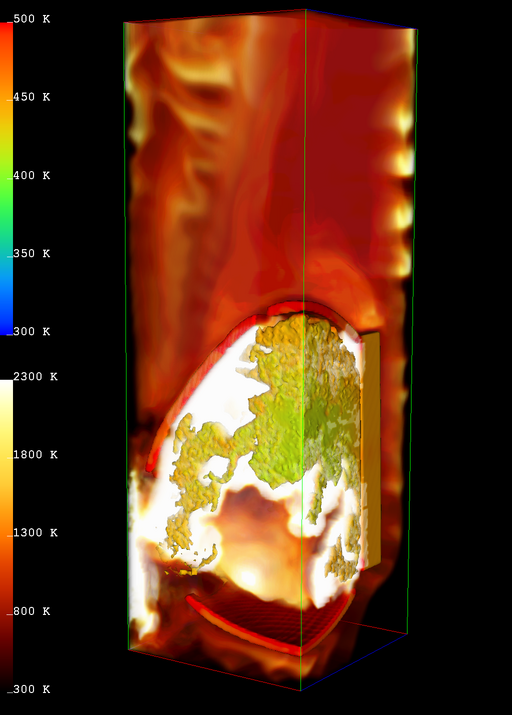
\includegraphics[width=\paperwidth,height=\paperheight,%
keepaspectratio]{fire-container-explosion-scirun.png}%
\vfill
}}}

%-------------------------------------------------------
% Versioning
%-------------------------------------------------------
\makeatletter
\def\MyYear#1{%
  \def\yy@##1##2##3##4;{##3##4}%
  \expandafter\yy@#1;
}
\def\MyMonth#1{%
  \def\yy@##1;{0##1}%
  \def\yy@##1##2;{##1##2}%
  \expandafter\yy@#1;
}
\def\MyDay#1{%
  \def\yy@##1;{0##1}%
  \def\yy@##1##2;{##1##2}%
  \expandafter\yy@#1;
}
\makeatother
\newcommand{\version}{Version \MyYear{\the\year}.\MyMonth{\the\month}.\MyDay{\the\day}}



%----------------------------------------------------------------------------------------
%	VARIOUS REQUIRED PACKAGES
%----------------------------------------------------------------------------------------

\usepackage{titlesec} % Allows customization of titles

%\usepackage{graphicx} % Required for including pictures
%\graphicspath{{./Pictures/}} % Specifies the directory where pictures are stored

\usepackage{lipsum} % Inserts dummy text

\usepackage{tikz} % Required for drawing custom shapes

\usepackage[english]{babel} % English language/hyphenation

\usepackage{enumitem} % Customize lists
\setlist{nolistsep} % Reduce spacing between bullet points and numbered lists

\usepackage{booktabs} % Required for nicer horizontal rules in tables

\usepackage{eso-pic} % Required for specifying an image background in the title page

%----------------------------------------------------------------------------------------
%	MAIN TABLE OF CONTENTS
%----------------------------------------------------------------------------------------

\usepackage{titletoc} % Required for manipulating the table of contents

\contentsmargin{0cm} % Removes the default margin

% Chapter text styling
\titlecontents{chapter}[1.25cm] % Indentation
{\addvspace{15pt}\large\sffamily\bfseries} % Spacing and font options for chapters
{\color{ocre!60}\contentslabel[\Large\thecontentslabel]{1.25cm}\color{ocre}} % Chapter number
{}  
{\color{ocre!60}\normalsize\sffamily\bfseries\;\titlerule*[.5pc]{.}\;\thecontentspage} % Page number

% Section text styling
\titlecontents{section}[1.55cm] % Indentation
{\addvspace{5pt}\sffamily} % Spacing and font options for sections
{\contentslabel[\thecontentslabel]{1.25cm}} % Section number
{}
{\sffamily\hfill\color{black}\thecontentspage} % Page number
[]

% Subsection text styling
\titlecontents{subsection}[1.85cm] % Indentation
{\addvspace{1pt}\sffamily\small} % Spacing and font options for subsections
{\contentslabel[\thecontentslabel]{1.25cm}} % Subsection number
{}
{\sffamily\;\titlerule*[.5pc]{.}\;\thecontentspage} % Page number
[] 

%----------------------------------------------------------------------------------------
%	MINI TABLE OF CONTENTS IN CHAPTER HEADS
%----------------------------------------------------------------------------------------

% Section text styling
\titlecontents{lsection}[0em] % Indendating
{\footnotesize\sffamily} % Font settings
{}
{}
{}

% Subsection text styling
\titlecontents{lsubsection}[.5em] % Indentation
{\normalfont\footnotesize\sffamily} % Font settings
{}
{}
{}
 
%----------------------------------------------------------------------------------------
%	PAGE HEADERS
%----------------------------------------------------------------------------------------

\usepackage{fancyhdr} % Required for header and footer configuration

\pagestyle{fancy}
\renewcommand{\chaptermark}[1]{\markboth{\sffamily\normalsize\bfseries #1}{}} % Chapter text font settings
\renewcommand{\sectionmark}[1]{\markright{\sffamily\normalsize\thesection\hspace{5pt}#1}{}} % Section text font settings
\fancyhf{} \fancyhead[LE,RO]{\sffamily\normalsize\thepage} % Font setting for the page number in the header
\fancyhead[LO]{\rightmark} % Print the nearest section name on the left side of odd pages
\fancyhead[RE]{\leftmark} % Print the current chapter name on the right side of even pages
\renewcommand{\headrulewidth}{0.5pt} % Width of the rule under the header
\addtolength{\headheight}{2.5pt} % Increase the spacing around the header slightly
\renewcommand{\footrulewidth}{0pt} % Removes the rule in the footer
\fancypagestyle{plain}{\fancyhead{}\renewcommand{\headrulewidth}{0pt}} % Style for when a plain pagestyle is specified

% Removes the header from odd empty pages at the end of chapters
\makeatletter
\renewcommand{\cleardoublepage}{
\clearpage\ifodd\c@page\else
\hbox{}
\vspace*{\fill}
\thispagestyle{empty}
\newpage
\fi}

%----------------------------------------------------------------------------------------
%	THEOREM STYLES
%----------------------------------------------------------------------------------------

\usepackage{amsmath} % For including math equations, theorems, symbols, etc
\usepackage{amsfonts} % For including math equations, theorems, symbols, etc
%\usepackage{amssymb} % For including math equations, theorems, symbols, etc
\usepackage{amsthm} % For including math equations, theorems, symbols, etc

\newcommand{\intoo}[2]{\mathopen{]}#1\,;#2\mathclose{[}}
\newcommand{\ud}{\mathop{\mathrm{{}d}}\mathopen{}}
\newcommand{\intff}[2]{\mathopen{[}#1\,;#2\mathclose{]}}
\newtheorem{notation}{Notation}[chapter]

\newtheoremstyle{ocrenum} % Theorem style name
{7pt} % Space above
{7pt} % Space below
{\normalfont} % Body font
{} % Indent amount
{\small\bf\sffamily\color{ocre}} % Theorem head font
{\;\;} % Punctuation after theorem head
{0.25em} % Space after theorem head
{\small\sffamily\color{ocre}\thmname{#1}\thmnumber{\@ifnotempty{#1}{ }\@upn{#2}} % Theorem text (e.g. Theorem 2.1)
\thmnote{\ {\the\thm@notefont\sffamily\bfseries\color{black}--- #3.}}} % Optional theorem note
\renewcommand{\qedsymbol}{$\blacksquare$} % Optional qed square

\newtheoremstyle{blacknumex} % Theorem style name
{7pt} % Space above
{7pt} % Space below
{\normalfont} % Body font
{} % Indent amount
{\small\bf\sffamily} % Theorem head font
{\;\;} % Punctuation after theorem head
{0.25em} % Space after theorem head
{\small\sffamily{\tiny\ensuremath{\blacksquare}}\ \thmname{#1}\thmnumber{\@ifnotempty{#1}{ }\@upn{#2}} % Theorem text (e.g. Theorem 2.1)
\thmnote{\ {\the\thm@notefont\sffamily\bfseries--- #3.}}} % Optional theorem note

\newtheoremstyle{blacknum} % Theorem style name
{7pt} % Space above
{7pt} % Space below
{\normalfont} % Body font
{} % Indent amount
{\small\bf\sffamily} % Theorem head font
{\;\;} % Punctuation after theorem head
{0.25em} % Space after theorem head
{\small\sffamily\thmname{#1}\thmnumber{\@ifnotempty{#1}{ }\@upn{#2}} % Theorem text (e.g. Theorem 2.1)
\thmnote{\ {\the\thm@notefont\sffamily\bfseries--- #3.}}} % Optional theorem note
\makeatother

% Defines the theorem text style for each type of theorem to one of the three styles above
\theoremstyle{ocrenum}
\newtheorem{theoremeT}{Theorem}[chapter]
\newtheorem{proposition}{Proposition}[chapter]
\newtheorem{problem}{Problem}[chapter]
\newtheorem{exerciseT}{Exercise}[chapter]
\theoremstyle{blacknumex}
\newtheorem{exampleT}{Example}[chapter]
\theoremstyle{blacknum}
\newtheorem{vocabulary}{Vocabulary}[chapter]
\newtheorem{definitionT}{Definition}[chapter]
\newtheorem{corollaryT}{Corollary}[chapter]

%----------------------------------------------------------------------------------------
%	DEFINITION OF COLORED BOXES
%----------------------------------------------------------------------------------------

\RequirePackage[framemethod=default]{mdframed} % Required for creating the theorem, definition, exercise and corollary boxes

% Theorem box
\newmdenv[skipabove=7pt,
skipbelow=7pt,
backgroundcolor=black!5,
linecolor=ocre,
innerleftmargin=5pt,
innerrightmargin=5pt,
innertopmargin=5pt,
leftmargin=0cm,
rightmargin=0cm,
innerbottommargin=5pt]{tBox}

% Exercise box	  
\newmdenv[skipabove=7pt,
skipbelow=7pt,
rightline=false,
leftline=true,
topline=false,
bottomline=false,
backgroundcolor=ocre!10,
linecolor=ocre,
innerleftmargin=5pt,
innerrightmargin=5pt,
innertopmargin=5pt,
innerbottommargin=5pt,
leftmargin=0cm,
rightmargin=0cm,
linewidth=4pt]{eBox}	

% Definition box
\newmdenv[skipabove=10pt,
skipbelow=10pt,
rightline=false,
leftline=true,
topline=false,
bottomline=false,
linecolor=ocre,
innerleftmargin=5pt,
innerrightmargin=5pt,
innertopmargin=0pt,
leftmargin=0cm,
rightmargin=0cm,
linewidth=4pt,
innerbottommargin=0pt]{dBox}	

% Corollary box
\newmdenv[skipabove=7pt,
skipbelow=7pt,
rightline=false,
leftline=true,
topline=false,
bottomline=false,
linecolor=gray,
backgroundcolor=black!5,
innerleftmargin=5pt,
innerrightmargin=5pt,
innertopmargin=5pt,
leftmargin=0cm,
rightmargin=0cm,
linewidth=4pt,
innerbottommargin=5pt]{cBox}				  
		  

% Creates an environment for each type of theorem and assigns it a theorem text style from the "Theorem Styles" section above and a colored box from above
\newenvironment{theorem}{\begin{tBox}\begin{theoremeT}}{\end{theoremeT}\end{tBox}}
\newenvironment{exercise}{\begin{eBox}\begin{exerciseT}}{\hfill{\color{ocre}\tiny\ensuremath{\blacksquare}}\end{exerciseT}\end{eBox}}				  
\newenvironment{definition}{\begin{dBox}\begin{definitionT}}{\end{definitionT}\end{dBox}}	
\newenvironment{example}{\begin{exampleT}}{\hfill{\tiny\ensuremath{\blacksquare}}\end{exampleT}}		
\newenvironment{corollary}{\begin{cBox}\begin{corollaryT}}{\end{corollaryT}\end{cBox}}	

%----------------------------------------------------------------------------------------
%	REMARK ENVIRONMENT
%----------------------------------------------------------------------------------------

\newenvironment{remark}{\par\vskip10pt\small % Vertical white space above the remark and smaller font size
\begin{list}{}{
\leftmargin=35pt % Indentation on the left
\rightmargin=25pt}\item\ignorespaces % Indentation on the right
\makebox[-2.5pt]{\begin{tikzpicture}[overlay]
\node[draw=ocre!60,line width=1pt,circle,fill=ocre!25,font=\sffamily\bfseries,inner sep=2pt,outer sep=0pt] at (-15pt,0pt){\textcolor{ocre}{R}};\end{tikzpicture}} % Orange R in a circle
\advance\baselineskip -1pt}{\end{list}\vskip5pt} % Tighter line spacing and white space after remark

%----------------------------------------------------------------------------------------
%	SECTION NUMBERING IN THE MARGIN
%----------------------------------------------------------------------------------------

\makeatletter
\renewcommand{\@seccntformat}[1]{\llap{\textcolor{ocre}{\csname the#1\endcsname}\hspace{1em}}}                    
\renewcommand{\section}{\@startsection{section}{1}{\z@}
{-4ex \@plus -1ex \@minus -.4ex}
{1ex \@plus.2ex }
{\normalfont\large\sffamily\bfseries}}
\renewcommand{\subsection}{\@startsection {subsection}{2}{\z@}
{-3ex \@plus -0.1ex \@minus -.4ex}
{0.5ex \@plus.2ex }
{\normalfont\sffamily\bfseries}}
\renewcommand{\subsubsection}{\@startsection {subsubsection}{3}{\z@}
{-2ex \@plus -0.1ex \@minus -.2ex}
{0.2ex \@plus.2ex }
{\color{teal}\normalfont\small\sffamily\bfseries}}                        
\renewcommand\paragraph{\@startsection{paragraph}{4}{\z@}
{-2ex \@plus-.2ex \@minus .2ex}
{0.1ex}
{\normalfont\small\sffamily\bfseries}}

%----------------------------------------------------------------------------------------
%	CHAPTER HEADINGS
%----------------------------------------------------------------------------------------

\newcommand{\thechapterimage}{}
\newcommand{\chapterimage}[1]{\renewcommand{\thechapterimage}{#1}}
\def\thechapter{\arabic{chapter}}
\def\@makechapterhead#1{
\thispagestyle{empty}
{\centering \normalfont\sffamily
\ifnum \c@secnumdepth >\m@ne
\if@mainmatter
\startcontents
\begin{tikzpicture}[remember picture,overlay]
\node at (current page.north west)
{\begin{tikzpicture}[remember picture,overlay]

\node[anchor=north west,inner sep=0pt] at (14,-0.5) {\includegraphics[width=0.3\paperwidth]{\thechapterimage}};

%Commenting the 3 lines below removes the small contents box in the chapter heading
%\draw[fill=white,opacity=.6] (1cm,0) rectangle (8cm,-7cm);
%\node[anchor=north west] at (1cm,.25cm) {\parbox[t][8cm][t]{6.5cm}{\huge\bfseries\flushleft \printcontents{l}{1}{\setcounter{tocdepth}{2}}}};

\draw[anchor=west] (5cm,-8cm) node [rounded corners=25pt,fill=white,fill opacity=1.0,text opacity=1,draw=ocre,draw opacity=1,line width=2pt,inner sep=15pt]{\huge\sffamily\bfseries\textcolor{black}{\thechapter\ ---\ #1\vphantom{plPQq}\makebox[22cm]{}}};
\end{tikzpicture}};
\end{tikzpicture}}\par\vspace*{200\p@}
\fi
\fi
}
\def\@makeschapterhead#1{
\thispagestyle{empty}
{\centering \normalfont\sffamily
\ifnum \c@secnumdepth >\m@ne
\if@mainmatter
\startcontents
\begin{tikzpicture}[remember picture,overlay]
\node at (current page.north west)
{\begin{tikzpicture}[remember picture,overlay]
\node[anchor=north west] at (14,-0.5) {\includegraphics[width=0.3\paperwidth]{\thechapterimage}};
\draw[anchor=west] (5cm,-8cm) node [rounded corners=25pt,fill=white,opacity=.7,inner sep=15.5pt]{\huge\sffamily\bfseries\textcolor{black}{\vphantom{plPQq}\makebox[22cm]{}}};
\draw[anchor=west] (5cm,-8cm) node [rounded corners=25pt,draw=ocre,line width=2pt,inner sep=15pt]{\huge\sffamily\bfseries\textcolor{black}{#1\vphantom{plPQq}\makebox[22cm]{}}};
\end{tikzpicture}};
\end{tikzpicture}}\par\vspace*{200\p@}
\fi
\fi
}
\makeatother

\newcommand{\AuthorNote}[1]{{\color{authorNoteColor} \sffamily{\textbf{#1}}}}

\newcommand{\Vaango}{\textsc{Vaango}\,}
\newcommand{\Uintah}{\textsc{Uintah}\,}
\newcommand{\MPM}{\textsc{MPM}\,}
\newcommand{\ICE}{\textsc{ICE}\,}
\newcommand{\MPMICE}{\textsc{MPMICE}\,}
\newcommand{\Arena}{\textsc{Arena}\,}
\newcommand{\Visit}{\textsc{VisIt}\,}
\newcommand{\Parsim}{\textsc{ParSim}\,}
\newcommand{\Textsfc}[1]{{\OliveD \textsf{#1}}\,}
\newcommand{\Textbfc}[1]{{\Pink \textsf{#1}}\,}
\newcommand{\Textttc}[1]{{\DarkGreen \texttt{#1}}\,}

%Wide bar
\newcommand{\overbar}[1]{\mkern 1.5mu\overline{\mkern-1.5mu#1\mkern-1.5mu}\mkern 1.5mu}
\renewcommand{\bar}[1]{\overbar{#1}}
\renewcommand{\widehat}[1]{\hat{#1}}

%__________________________________
% new commands for all sections
\newcommand{\BBComment}[1]{ \marginpar{{\scriptsize \color{red} #1 }}}
\newcommand{\red}[1]{\color{red} {#1} \color{black}}
\newcommand{\TT}[1]{\ensuremath{\tt{#1}\normalfont}}

% MPM & ICE
\newcommand{\tn}[1]{\mbox{\ensuremath{\mathbf{#1}}}}
\newcommand{\sig}{\mbox{\boldmath $\sigma \!\!$ \unboldmath}}
\newcommand{\bnabla} {\mbox {\boldmath $\nabla \!\!$ \unboldmath}}
\newcommand{\taubold} {\mbox{\boldmath $\tau \!\!$ \unboldmath}}
\newcommand{\f}{\ensuremath{f^{\theta}_r} }

\newcommand{\Texp}{\rm{exp}}
\newcommand{\Delt}{\ensuremath{\Delta t}}
\newcommand{\Epj}{\ensuremath{\epsilon_{p,j}}}
\newcommand{\Epo}{\ensuremath{\epsilon_{p,0}}}
\newcommand{\lambdadot}{\ensuremath{\dot{\lambda}}}
\def\bfE{{\bf E}}

\newcommand{\hangp}[1]{\makebox[0pt][r]{(}#1\makebox[0pt][l]{)}} % New command to create parentheses around text in tables which take up no horizontal space - this improves column spacing
\newcommand{\hangstar}{\makebox[0pt][l]{*}} % New command to create asterisks in tables which take up no horizontal space - this improves column spacing

\newcommand{\monthyear}{\ifcase\month\or January\or February\or March\or April\or May\or June\or July\or August\or September\or October\or November\or December\fi\space\number\year} % A command to print the current month and year

\newcommand{\blankpage}{\newpage\hbox{}\thispagestyle{empty}\newpage} % Command to insert a blank page

\def\rmd{{\rm d}}
\def\rme{{\rm e}}
\def\rmf{{\rm f}}
\def\rmr{{\rm r}}
\def\rmR{{\rm R}}
\def\rms{{\rm s}}
\def\bfd{{\bf d}}
\def\bfE{{\bf E}}
\def\bfF{{\bf F}}
\def\bff{{\bf f}}
\def\bfg{{\bf g}}
\def\bfI{{\bf I}}
\def\bfj{{\bf j}}
\def\bfm{{\bf m}}
\def\bfr{{\bf r}}
\def\bfx{{\bf x}}
\def\bfu{{\bf u}}
\def\rmg{{\rm g}}
\def\bfa{{\bf a}}
\def\bfG{{\bf G}}
\def\bfv{{\bf v}}
\def\tdot{{\textstyle\cdot}}

\pdfcompresslevel=9
%\raggedright

\newcommand{\handout}[3]{
        \begin{center}
         % \copyright 
          Biswajit Banerjee \hspace{4.2in} University of Utah\\
          \vspace{10pt}
          {\Large\bf Waves in Composites and Metamaterials}\\
          \vspace{6pt}
          (Instructor: Prof. G. W. Milton)
        \end{center}
        \vspace{8pt}\noindent
        %\begin{center}
        {\underline{\makebox[7.0in]{\large\bf\noindent
                \makebox[1.5in][l]{#1~~~} \hfill {~~~#2~~~} \hfill
                \makebox[1.5in][r]{~~~#3}}}}
        %\end{center}
        }

\newcommand{\heading}[1]{
        \begin{center}{\large\bf{#1}}\end{center}}

\newcommand{\subheading}[1]{
        \begin{center}{\normalsize\bf{#1}}\end{center}}

\newcommand{\subsubheading}[1]{
        \begin{center}{\small\bf{#1}}\end{center}}

\newcommand{\Heading}[1]{
        \vspace{12pt}\begin{center}{\Large\bf{#1}}\end{center}}

\newcommand{\Subheading}[1]{
        \vspace{8pt}\begin{center}{\large\bf{#1}}\end{center}}

\newcommand{\Jump}[1]{\ensuremath{\llbracket#1\rrbracket}}
\newcommand{\Blimitx}[1]{\ensuremath{\left[#1\right]_{x_a}^{x_b}}}
\newcommand{\Deriv}[2]{\ensuremath{\cfrac{d#1}{d#2}}}
\newcommand{\MDeriv}[2]{\ensuremath{\cfrac{D#1}{D#2}}}
\newcommand{\DDeriv}[2]{\ensuremath{\cfrac{d^2#1}{d#2^2}}}
\newcommand{\DDDeriv}[2]{\ensuremath{\cfrac{d^3#1}{d#2^3}}}
\newcommand{\DDDDeriv}[2]{\ensuremath{\cfrac{d^4#1}{d#2^4}}}
\newcommand{\Intx}{\ensuremath{\int_{x_a}^{x_b}}}
\newcommand{\IntX}{\ensuremath{\int_{X_a}^{X_b}}}
\newcommand{\Intiso}{\ensuremath{\int_{-1}^{1}}}
\newcommand{\IntOmegaA}{\ensuremath{\int_{\Omega_0}}}
\newcommand{\IntOmega}{\ensuremath{\int_{\Omega}}}
\newcommand{\IntDOmega}{\ensuremath{\int_{\partial\Omega}}}
\newcommand{\Norm}[2]{\ensuremath{\left\lVert#1\right\rVert_{#2}}}
\newcommand{\norm}[1]{\ensuremath{\left\lVert#1\right\rVert}}
\newcommand{\Var}[1]{\ensuremath{\delta #1}}
\newcommand{\DelT}{\ensuremath{\Delta t}}
\newcommand{\CalA}{\ensuremath{\mathcal{A}}}
\newcommand{\CalB}{\ensuremath{\mathcal{B}}}
\newcommand{\CalC}{\ensuremath{\mathcal{C}}}
\newcommand{\CalF}{\ensuremath{\mathcal{F}}}
\newcommand{\CalL}{\ensuremath{\mathcal{L}}}
\newcommand{\CalM}{\ensuremath{\mathcal{M}}}
\newcommand{\BCalM}{\ensuremath{\boldsymbol{\CalM}}}
\newcommand{\CalN}{\ensuremath{\mathcal{N}}}
\newcommand{\CalP}{\ensuremath{\mathcal{P}}}
\newcommand{\CalS}{\ensuremath{\mathcal{S}}}
\newcommand{\BCalS}{\ensuremath{\boldsymbol{\CalS}}}
\newcommand{\CalT}{\ensuremath{\mathcal{T}}}
\newcommand{\CalV}{\ensuremath{\mathcal{V}}}
\newcommand{\CalW}{\ensuremath{\mathcal{W}}}
\newcommand{\CalX}{\ensuremath{\mathcal{X}}}
\newcommand{\Comp}[2]{\ensuremath{#1 \circ #2}}
\newcommand{\Map}[3]{\ensuremath{#1 : #2 \rightarrow #3}}
\newcommand{\MapTo}[3]{\ensuremath{#1 : #2 \mapsto #3}}
\newcommand{\Real}[1]{\ensuremath{\mathbb{R}^{#1}}}
\newcommand{\Ve}{\ensuremath{\varepsilon}}
\newcommand{\BHat}[1]{\ensuremath{\widehat{\boldsymbol{#1}}}}
\newcommand{\BTx}{\ensuremath{\tilde{\boldsymbol{x}}}}
\newcommand{\Beh}{\ensuremath{\hat{\boldsymbol{e}}}}
\newcommand{\BHex}{\ensuremath{\hat{\boldsymbol{e}}_1}}
\newcommand{\BHey}{\ensuremath{\hat{\boldsymbol{e}}_2}}
\newcommand{\BHez}{\ensuremath{\hat{\boldsymbol{e}}_3}}
\newcommand{\BHn}[1]{\ensuremath{\hat{\boldsymbol{n}}_{#1}}}
\newcommand{\BHe}[1]{\ensuremath{\hat{\boldsymbol{e}}_{#1}}}
\newcommand{\BHg}[1]{\ensuremath{\hat{\boldsymbol{g}}_{#1}}}
\newcommand{\BHG}[1]{\ensuremath{\hat{\boldsymbol{G}}_{#1}}}
\newcommand{\Hn}{\ensuremath{\hat{\boldsymbol{n}}}}
\newcommand{\Mba}{\ensuremath{\mathbf{a}}}
\newcommand{\Mbatilde}{\ensuremath{\widetilde{\mathbf{a}}}}
\newcommand{\Mbb}{\ensuremath{\mathbf{b}}}
\newcommand{\Mbd}{\ensuremath{\mathbf{d}}}
\newcommand{\Mbf}{\ensuremath{\mathbf{f}}}
\newcommand{\Mbn}{\ensuremath{\mathbf{n}}}
\newcommand{\Mbntilde}{\ensuremath{\widetilde{\mathbf{n}}}}
\newcommand{\Mbr}{\ensuremath{\mathbf{r}}}
\newcommand{\Mbu}{\ensuremath{\mathbf{u}}}
\newcommand{\Mbv}{\ensuremath{\mathbf{v}}}
\newcommand{\Mbx}{\ensuremath{\mathbf{x}}}
\newcommand{\MbA}{\ensuremath{\mathbf{A}}}
\newcommand{\MbB}{\ensuremath{\mathbf{B}}}
\newcommand{\MbC}{\ensuremath{\mathbf{C}}}
\newcommand{\MbD}{\ensuremath{\mathbf{D}}}
\newcommand{\MbH}{\ensuremath{\mathbf{H}}}
\newcommand{\MbHbar}{\ensuremath{\mathbf{\overline{H}}}}
\newcommand{\MbI}{\ensuremath{\mathbf{I}}}
\newcommand{\MbK}{\ensuremath{\mathbf{K}}}
\newcommand{\MbKbar}{\ensuremath{\overline{\mathbf{K}}}}
\newcommand{\MbKtilde}{\ensuremath{\widetilde{\mathbf{K}}}}
\newcommand{\MbM}{\ensuremath{\mathbf{M}}}
\newcommand{\MbN}{\ensuremath{\mathbf{N}}}
\newcommand{\MbP}{\ensuremath{\mathbf{P}}}
\newcommand{\MbPbar}{\ensuremath{\overline{\mathbf{P}}}}
\newcommand{\MbR}{\ensuremath{\mathbf{R}}}
\newcommand{\MbT}{\ensuremath{\mathbf{T}}}
\newcommand{\MbU}{\ensuremath{\mathbf{U}}}
\newcommand{\MbV}{\ensuremath{\mathbf{V}}}
\newcommand{\MbX}{\ensuremath{\mathbf{X}}}
\newcommand{\MbSig}{\ensuremath{\boldsymbol{\sigma}}}
\newcommand{\Mbone}{\ensuremath{\mathbf{1}}}
\newcommand{\Mbzero}{\ensuremath{\mathbf{0}}}
%\newcommand{\Mb}{\ensuremath{\left[\mathsf{b}\right]}}
%\newcommand{\Mu}{\ensuremath{\left[\mathsf{u}\right]}}
%\newcommand{\Mv}{\ensuremath{\left[\mathsf{v}\right]}}
%\newcommand{\Mw}{\ensuremath{\left[\mathsf{w}\right]}}
%\newcommand{\Mx}{\ensuremath{\left[\mathsf{x}\right]}}
\newcommand{\MA}{\ensuremath{\left[\mathsf{A}\right]}}
\newcommand{\MB}{\ensuremath{\left[\mathsf{B}\right]}}
\newcommand{\MC}{\ensuremath{\left[\mathsf{C}\right]}}
\newcommand{\MD}{\ensuremath{\left[\mathsf{D}\right]}}
\newcommand{\MH}{\ensuremath{\left[\mathsf{H}\right]}}
\newcommand{\MI}{\ensuremath{\left[\mathsf{I}\right]}}
\newcommand{\ML}{\ensuremath{\left[\mathsf{L}\right]}}
\newcommand{\MM}{\ensuremath{\left[\mathsf{M}\right]}}
\newcommand{\MN}{\ensuremath{\left[\mathsf{N}\right]}}
\newcommand{\MP}{\ensuremath{\left[\mathsf{P}\right]}}
\newcommand{\MQ}{\ensuremath{\left[\mathsf{Q}\right]}}
\newcommand{\MR}{\ensuremath{\left[\mathsf{R}\right]}}
\newcommand{\MT}{\ensuremath{\left[\mathsf{T}\right]}}
\newcommand{\MV}{\ensuremath{\left[\mathsf{V}\right]}}
%\newcommand{\Mone}{\ensuremath{\left[\mathsf{1}\right]}}
%\newcommand{\Mzero}{\ensuremath{\left[\mathsf{0}\right]}}
\newcommand{\SfA}{\ensuremath{\boldsymbol{\mathsf{A}}}}
\newcommand{\SfB}{\ensuremath{\boldsymbol{\mathsf{B}}}}
\newcommand{\SfC}{\ensuremath{\boldsymbol{\mathsf{C}}}}
\newcommand{\SfD}{\ensuremath{\boldsymbol{\mathsf{D}}}}
\newcommand{\SfI}{\ensuremath{\boldsymbol{\mathsf{I}}}}
\newcommand{\SfL}{\ensuremath{\boldsymbol{\mathsf{L}}}}
\newcommand{\Sfp}{\ensuremath{\boldsymbol{\mathsf{p}}}}
\newcommand{\SfP}{\ensuremath{\boldsymbol{\mathsf{P}}}}
\newcommand{\SfS}{\ensuremath{\boldsymbol{\mathsf{S}}}}
\newcommand{\SfT}{\ensuremath{\boldsymbol{\mathsf{T}}}}
\newcommand{\Msig}{\ensuremath{\left[\boldsymbol{\sigma}\right]}}
\newcommand{\Meps}{\ensuremath{\left[\boldsymbol{\varepsilon}\right]}}
\newcommand{\Ex}{\ensuremath{\boldsymbol{e}_1}}
\newcommand{\Ey}{\ensuremath{\boldsymbol{e}_2}}
\newcommand{\Ez}{\ensuremath{\boldsymbol{e}_3}}
\newcommand{\Exp}{\ensuremath{\boldsymbol{e}^{'}_1}}
\newcommand{\Eyp}{\ensuremath{\boldsymbol{e}^{'}_2}}
\newcommand{\Ezp}{\ensuremath{\boldsymbol{e}^{'}_3}}
\newcommand{\Ep}{\ensuremath{\varepsilon_p}}
\newcommand{\Epi}{\ensuremath{\varepsilon_{pi}}}
\newcommand{\Epdot}[1]{\ensuremath{\dot{\varepsilon}_{p#1}}}
\newcommand{\Epsxx}{\ensuremath{\varepsilon_{11}}}
\newcommand{\Epsyy}{\ensuremath{\varepsilon_{22}}}
\newcommand{\Epszz}{\ensuremath{\varepsilon_{33}}}
\newcommand{\Epsyz}{\ensuremath{\varepsilon_{23}}}
\newcommand{\Epszx}{\ensuremath{\varepsilon_{31}}}
\newcommand{\Epsxy}{\ensuremath{\varepsilon_{12}}}
\newcommand{\Sigxx}{\ensuremath{\sigma_{11}}}
\newcommand{\Sigyy}{\ensuremath{\sigma_{22}}}
\newcommand{\Sigzz}{\ensuremath{\sigma_{33}}}
\newcommand{\Sigyz}{\ensuremath{\sigma_{23}}}
\newcommand{\Sigzx}{\ensuremath{\sigma_{31}}}
\newcommand{\Sigxy}{\ensuremath{\sigma_{12}}}
\newcommand{\Eps}[1]{\ensuremath{\varepsilon_{#1}}}
\newcommand{\Sig}[1]{\ensuremath{\sigma_{#1}}}
\newcommand{\X}{\ensuremath{X_1}}
\newcommand{\Y}{\ensuremath{X_2}}
\newcommand{\Z}{\ensuremath{X_3}}
\newcommand{\erf}{\text{erf}}
\newcommand{\Xidot}{\ensuremath{\dot{\xi}}}
\newcommand{\Balpha}{\ensuremath{\boldsymbol{\alpha}}}
\newcommand{\Balphahat}{\ensuremath{\widehat{\boldsymbol{\alpha}}}}
\newcommand{\Bbeta}{\ensuremath{\boldsymbol{\beta}}}
\newcommand{\Beta}{\ensuremath{\boldsymbol{\eta}}}
\newcommand{\Bchi}{\ensuremath{\boldsymbol{\chi}}}
\newcommand{\Bpsi}{\ensuremath{\boldsymbol{\psi}}}
\newcommand{\Bveps}{\ensuremath{\boldsymbol{\varepsilon}}}
\newcommand{\BGamma}{\ensuremath{\boldsymbol{\mathit{\Gamma}}}}
\newcommand{\BGammahat}{\ensuremath{\boldsymbol{\mathit{\widehat{\Gamma}}}}}
%\newcommand{\BGammahat}{\ensuremath{\widehat{\BGamma}}}
\newcommand{\Bkappa}{\ensuremath{\boldsymbol{\kappa}}}
\newcommand{\Bbeps}{\ensuremath{\bar{\boldsymbol{\varepsilon}}}}
\newcommand{\Bnabla}{\ensuremath{\boldsymbol{\nabla}}}
\newcommand{\Bomega}{\ensuremath{\boldsymbol{\omega}}}
\newcommand{\BOmega}{\ensuremath{\boldsymbol{\Omega}}}
\newcommand{\Bsig}{\ensuremath{\boldsymbol{\sigma}}}
\newcommand{\Bsigbar}{\ensuremath{\overline{\boldsymbol{\sigma}}}}
\newcommand{\BSig}{\ensuremath{\boldsymbol{\Sigma}}}
\newcommand{\Btau}{\ensuremath{\boldsymbol{\tau}}}
\newcommand{\Bpi}{\ensuremath{\boldsymbol{\pi}}}
\newcommand{\Brho}{\ensuremath{\boldsymbol{\rho}}}
\newcommand{\Bvarphi}{\ensuremath{\boldsymbol{\varphi}}}
\newcommand{\phibar}{\ensuremath{\overline{\varphi}}}
\newcommand{\Blambda}{\ensuremath{\boldsymbol{\lambda}}}
\newcommand{\Btheta}{\ensuremath{\boldsymbol{\theta}}}
\newcommand{\Bthetav}{\ensuremath{\mathbf{\theta}}}
\newcommand{\Bgamma}{\ensuremath{\boldsymbol{\gamma}}}
\newcommand{\Bmu}{\ensuremath{\boldsymbol{\mu}}}
\newcommand{\Bxi}{\ensuremath{\boldsymbol{\xi}}}
\newcommand{\BPi}{\ensuremath{\boldsymbol{\Pi}}}
\newcommand{\Bone}{\ensuremath{\boldsymbol{\mathit{1}}}}
\newcommand{\Bonev}{\ensuremath{\boldsymbol{1}}}
\newcommand{\Bzero}{\ensuremath{\boldsymbol{0}}}
\newcommand{\BzeroT}{\ensuremath{\boldsymbol{\mathit{0}}}}
\newcommand{\Ba}{\ensuremath{\mathbf{a}}}
\newcommand{\Bb}{\ensuremath{\mathbf{b}}}
\newcommand{\BbT}{\ensuremath{\boldsymbol{b}}}
\newcommand{\Bc}{\ensuremath{\mathbf{c}}}
\newcommand{\Bd}{\ensuremath{\mathbf{d}}}
\newcommand{\BdT}{\ensuremath{\boldsymbol{d}}}
\newcommand{\Bdv}{\ensuremath{\mathbf{d}}}
\newcommand{\Be}{\ensuremath{\mathbf{e}}}
\newcommand{\BeT}{\ensuremath{\boldsymbol{e}}}
\newcommand{\Bf}{\ensuremath{\mathbf{f}}}
\newcommand{\Bg}{\ensuremath{\mathbf{g}}}
\newcommand{\Bh}{\ensuremath{\boldsymbol{h}}}
\newcommand{\Bhv}{\ensuremath{\mathbf{h}}}
\newcommand{\Bj}{\ensuremath{\mathbf{j}}}
\newcommand{\Bk}{\ensuremath{\mathbf{k}}}
\newcommand{\Bl}{\ensuremath{\mathbf{l}}}
\newcommand{\BlT}{\ensuremath{\boldsymbol{l}}}
\newcommand{\Bm}{\ensuremath{\mathbf{m}}}
\newcommand{\Bn}{\ensuremath{\mathbf{n}}}
\newcommand{\BnT}{\ensuremath{\boldsymbol{n}}}
\newcommand{\Bo}{\ensuremath{\mathbf{o}}}
\newcommand{\Bp}{\ensuremath{\mathbf{p}}}
\newcommand{\Bq}{\ensuremath{\mathbf{q}}}
\newcommand{\Br}{\ensuremath{\boldsymbol{r}}}
\newcommand{\Brv}{\ensuremath{\mathbf{r}}}
\newcommand{\Bs}{\ensuremath{\mathbf{s}}}
\newcommand{\BsT}{\ensuremath{\boldsymbol{s}}}
\newcommand{\Bsv}{\ensuremath{\mathbf{s}}}
\newcommand{\Bt}{\ensuremath{\mathbf{t}}}
\newcommand{\Bu}{\ensuremath{\mathbf{u}}}
\newcommand{\Bv}{\ensuremath{\mathbf{v}}}
\newcommand{\Bw}{\ensuremath{\mathbf{w}}}
\newcommand{\Bx}{\ensuremath{\mathbf{x}}}
\newcommand{\By}{\ensuremath{\mathbf{y}}}
\newcommand{\Bz}{\ensuremath{\mathbf{z}}}
\newcommand{\BA}{\ensuremath{\boldsymbol{A}}}
\newcommand{\BB}{\ensuremath{\boldsymbol{B}}}
\newcommand{\BBbar}{\ensuremath{\bar{\boldsymbol{B}}}}
\newcommand{\BC}{\ensuremath{\boldsymbol{C}}}
\newcommand{\BCbar}{\ensuremath{\bar{\boldsymbol{C}}}}
\newcommand{\Cbar}{\ensuremath{\bar{C}}}
\newcommand{\BD}{\ensuremath{\boldsymbol{D}}}
\newcommand{\BE}{\ensuremath{\boldsymbol{E}}}
\newcommand{\BF}{\ensuremath{\boldsymbol{F}}}
\newcommand{\BFbar}{\ensuremath{\bar{\boldsymbol{F}}}}
\newcommand{\Fbar}{\ensuremath{\bar{F}}}
\newcommand{\BG}{\ensuremath{\boldsymbol{G}}}
\newcommand{\BGv}{\ensuremath{\mathbf{G}}}
\newcommand{\BH}{\ensuremath{\boldsymbol{H}}}
\newcommand{\BI}{\ensuremath{\boldsymbol{I}}}
\newcommand{\BBI}{\ensuremath{\mathbb{I}}}
\newcommand{\BJ}{\ensuremath{\boldsymbol{J}}}
\newcommand{\BK}{\ensuremath{\boldsymbol{K}}}
\newcommand{\BL}{\ensuremath{\boldsymbol{L}}}
\newcommand{\BM}{\ensuremath{\boldsymbol{M}}}
\newcommand{\BNv}{\ensuremath{\mathbf{N}}}
\newcommand{\BN}{\ensuremath{\boldsymbol{N}}}
\newcommand{\BP}{\ensuremath{\boldsymbol{P}}}
\newcommand{\BBP}{\ensuremath{\mathbb{P}}}
\newcommand{\BQ}{\ensuremath{\boldsymbol{Q}}}
\newcommand{\BBQ}{\ensuremath{\mathbb{Q}}}
\newcommand{\BQv}{\ensuremath{\mathbf{Q}}}
\newcommand{\BR}{\ensuremath{\boldsymbol{R}}}
\newcommand{\BBR}{\ensuremath{\mathbb{R}}}
\newcommand{\BS}{\ensuremath{\boldsymbol{S}}}
\newcommand{\BSmat}{\ensuremath{\mathbf{S}}}
\newcommand{\BT}{\ensuremath{\boldsymbol{T}}}
\newcommand{\BTv}{\ensuremath{\mathbf{T}}}
\newcommand{\BU}{\ensuremath{\boldsymbol{U}}}
\newcommand{\BV}{\ensuremath{\boldsymbol{V}}}
\newcommand{\BW}{\ensuremath{\boldsymbol{W}}}
\newcommand{\BX}{\ensuremath{\mathbf{X}}}
\newcommand{\BXT}{\ensuremath{\boldsymbol{X}}}
\newcommand{\BY}{\ensuremath{\boldsymbol{Y}}}
\newcommand{\BZ}{\ensuremath{\boldsymbol{Z}}}
\newcommand{\Trial}{\ensuremath{\text{trial}}}
\newcommand{\Tiso}{\ensuremath{\text{iso}}}
\newcommand{\Tint}{\ensuremath{\text{int}}}
\newcommand{\Text}{\ensuremath{\text{ext}}}
\newcommand{\Tkin}{\ensuremath{\text{kin}}}
\newcommand{\Tbody}{\ensuremath{\text{body}}}
\newcommand{\Tinert}{\ensuremath{\text{inertial}}}
\newcommand{\Telast}{\ensuremath{\text{elastic}}}
\newcommand{\Ttop}{\ensuremath{\text{top}}}
\newcommand{\Tbot}{\ensuremath{\text{bot}}}
\newcommand{\Tcore}{\ensuremath{\text{core}}}
\newcommand{\Teq}{\ensuremath{\text{eq}}}
\newcommand{\Tface}{\ensuremath{\text{face}}}
\newcommand{\Tpot}{\ensuremath{\text{pot}}}
\newcommand{\Tright}{\ensuremath{\text{right}}}
\newcommand{\Tleft}{\ensuremath{\text{left}}}
\newcommand{\Tdrag}{\ensuremath{\text{drag}}}
\newcommand{\Tmin}{\ensuremath{\text{min}}}
\newcommand{\Tmax}{\ensuremath{\text{max}}}
\newcommand{\Tsat}{\ensuremath{\text{sat}}}
\newcommand{\Tapex}{\ensuremath{\text{apex}}}
\newcommand{\Tref}{\ensuremath{\text{ref}}}
\newcommand{\Tnew}{\ensuremath{\text{new}}}
\newcommand{\Told}{\ensuremath{\text{old}}}
\newcommand{\Tin}{\ensuremath{\text{in}}}
\newcommand{\Tlocal}{\ensuremath{\text{local}}}
\newcommand{\Tmid}{\ensuremath{\text{mid}}}
\newcommand{\Tout}{\ensuremath{\text{out}}}
\newcommand{\Tratio}{\ensuremath{\text{ratio}}}
\newcommand{\Tsub}{\ensuremath{\text{sub}}}
\newcommand{\Te}{\ensuremath{\text{e}}}
\newcommand{\Tp}{\ensuremath{\text{p}}}
\newcommand{\Tn}{\ensuremath{\text{n}}}
\newcommand{\Tpeak}{\ensuremath{\text{peak}}}
\newcommand{\Trot}{\ensuremath{\text{rot}}}
\newcommand{\Tor}{\ensuremath{\text{or}}}
\newcommand{\Tr}{\ensuremath{\text{tr}}}
\newcommand{\Dev}{\ensuremath{\text{dev}}}
\newcommand{\Ttt}{\ensuremath{\text{tt}}}
\newcommand{\Ttb}{\ensuremath{\text{tb}}}
\newcommand{\Tbt}{\ensuremath{\text{bt}}}
\newcommand{\Tbb}{\ensuremath{\text{bb}}}
\newcommand{\Ttc}{\ensuremath{\text{tc}}}
\newcommand{\Tbc}{\ensuremath{\text{bc}}}
\newcommand{\Tdev}{\ensuremath{\text{dev}}}
\newcommand{\Tvol}{\ensuremath{\text{vol}}}
\newcommand{\Half}{\ensuremath{\tfrac{1}{2}}}
\newcommand{\SThr}{\ensuremath{\sqrt{3}}}
\newcommand{\STT}{\ensuremath{\frac{\sqrt{3}}{2}}}
\newcommand{\Third}{\ensuremath{\tfrac{1}{3}}}
\newcommand{\TwoThird}{\ensuremath{\tfrac{2}{3}}}
\newcommand{\Inner}[2]{\ensuremath{\langle#1,~#2\rangle}}
\newcommand{\Bcross}[2]{\ensuremath{#1\boldsymbol{\times}#2}}
\newcommand{\Bdot}[2]{\ensuremath{#1\cdot#2}}
\newcommand{\Dyad}[2]{\ensuremath{#1\boldsymbol{\otimes}#2}}
\newcommand{\Grad}[1]{\ensuremath{\Bnabla #1}}
\newcommand{\Gradp}[1]{\ensuremath{\Bnabla' #1}}
\newcommand{\Grads}[1]{\ensuremath{\Bnabla_s #1}}
\newcommand{\Grady}[1]{\ensuremath{\Bnabla_y #1}}
\newcommand{\Lap}[1]{\ensuremath{\nabla^2 #1}}
\newcommand{\Biharm}[1]{\ensuremath{\nabla^4 #1}}
\newcommand{\Div}[1]{\ensuremath{\Bdot{\Bnabla}{#1}}}
\newcommand{\Divp}[1]{\ensuremath{\Bdot{\Bnabla'}{#1}}}
\newcommand{\Divy}[1]{\ensuremath{\Bdot{\Bnabla_y}{#1}}}
\newcommand{\Curl}[1]{\ensuremath{\Bcross{\Bnabla}{#1}}}
\newcommand{\Curlp}[1]{\ensuremath{\Bcross{\Bnabla'}{#1}}}
\newcommand{\Curls}[1]{\ensuremath{\Bcross{\Bnabla_s}{#1}}}
\newcommand{\Curly}[1]{\ensuremath{\Bcross{\Bnabla_y}{#1}}}
\newcommand{\Gradu}{\ensuremath{\Grad{\Bu}}}
\newcommand{\Divu}{\ensuremath{\Div{\Bu}}}
\newcommand{\Curlu}{\ensuremath{\Curl{\Bu}}}
\newcommand{\Gradv}{\ensuremath{\Grad{\Bv}}}
\newcommand{\Divv}{\ensuremath{\Div{\Bv}}}
\newcommand{\Curlv}{\ensuremath{\Curl{\Bv}}}
\newcommand{\Dualn}{\ensuremath{\Bdual{\Bn}{\Bn}}}
\newcommand{\Over}[1]{\ensuremath{\frac{1}{#1}}}
\newcommand{\Diff}[2]{\ensuremath{\frac{d #1}{d #2}}}
\newcommand{\Partial}[2]{\ensuremath{\frac{\displaystyle\partial #1}{\displaystyle\partial #2}}}
\newcommand{\PPartial}[2]{\ensuremath{\frac{\partial^2 #1}{\partial #2^2}}}
\newcommand{\PPartialA}[3]{\ensuremath{\frac{\partial^2 #1}{\partial #2\partial#3}}}
\newcommand{\FPartial}[2]{\ensuremath{\frac{\partial^4 #1}{\partial #2^4}}}
\newcommand{\FPartialA}[3]{\ensuremath{\frac{\partial^4 #1}{\partial #2^2
         \partial #3^2}}}
\newcommand{\DotMbT}{\ensuremath{\dot{\MbT}}}
\newcommand{\TildeMbT}{\ensuremath{\widetilde{\MbT}}}
\newcommand{\BarT}{\ensuremath{\overline{T}}}
\newcommand{\Barq}{\ensuremath{\overline{q}}}
\newcommand{\Domega}{\ensuremath{\partial{\Omega}}}
\newcommand{\Av}[1]{\ensuremath{\left\langle#1\right\rangle}}
\newcommand{\AvSig}{\ensuremath{\langle\Bsig\rangle}}
\newcommand{\AvTau}{\ensuremath{\langle\Btau\rangle}}
\newcommand{\AvP}{\ensuremath{\langle\BP\rangle}}
\newcommand{\AvEps}{\ensuremath{\langle\Beps\rangle}}
\newcommand{\AvEpsdot}{\ensuremath{\langle\dot{\Beps}\rangle}}
\newcommand{\AvDisp}{\ensuremath{\langle\Bu\rangle}}
\newcommand{\AvF}{\ensuremath{\langle\BF\rangle}}
\newcommand{\AvFdot}{\ensuremath{\langle\dot{\BF}\rangle}}
\newcommand{\Avl}{\ensuremath{\overline{\Bl}}}
\newcommand{\AvSigBar}{\ensuremath{\overline{\Bsig}}}
\newcommand{\AvTauBar}{\ensuremath{\overline{\Btau}}}
\newcommand{\AvOmega}{\ensuremath{\langle\Bomega\rangle}}
\newcommand{\AvGradu}{\ensuremath{\langle\Gradu\rangle}}
\newcommand{\AvGradudot}{\ensuremath{\langle\Grad{\dot{\Bu}}\rangle}}
\newcommand{\AvGradv}{\ensuremath{\langle\Gradv\rangle}}
\newcommand{\AvPower}{\ensuremath{\langle\Bsig:\Gradv\rangle}}
\newcommand{\AvPowerInf}{\ensuremath{\langle\Bsig:\dot{\Beps}\rangle}}
\newcommand{\AvWorkInf}{\ensuremath{\langle\Bsig:\Beps\rangle}}
\newcommand{\AvPowerPF}{\ensuremath{\langle\BP^T:\dot{\BF}\rangle}}
\newcommand{\DA}{\ensuremath{\text{dA}}}
\newcommand{\DAvec}{\ensuremath{\text{d}\mathbf{A}}}
\newcommand{\Da}{\ensuremath{\text{da}}}
\newcommand{\Davec}{\ensuremath{\text{d}\mathbf{a}}}
\newcommand{\DV}{\ensuremath{\text{dV}}}
\newcommand{\Dv}{\ensuremath{\text{dv}}}
\newcommand{\BCe}{\ensuremath{\mathcal{E}}}
\newcommand{\GradX}[1]{\ensuremath{\Bnabla_{\mkern-3.7mu 0}#1}}
\newcommand{\DivX}[1]{\ensuremath{\Bdot{\Bnabla_0}{#1}}}
\newcommand{\Bxdot}{\ensuremath{\dot{\Bx}}}
\newcommand{\BFdot}{\ensuremath{\dot{\BF}}}
\newcommand{\BAv}{\ensuremath{\mathbf{A}}}
\newcommand{\BBv}{\ensuremath{\mathbf{B}}}
\newcommand{\BDv}{\ensuremath{\mathbf{D}}}
\newcommand{\BEv}{\ensuremath{\mathbf{E}}}
\newcommand{\BFv}{\ensuremath{\mathbf{F}}}
\newcommand{\BHv}{\ensuremath{\mathbf{H}}}
\newcommand{\BJv}{\ensuremath{\mathbf{J}}}
\newcommand{\BMv}{\ensuremath{\mathbf{M}}}
\newcommand{\BPv}{\ensuremath{\mathbf{P}}}
\newcommand{\BRv}{\ensuremath{\mathbf{R}}}
\newcommand{\BVv}{\ensuremath{\mathbf{V}}}
\newcommand{\Bdelta}{\ensuremath{\boldsymbol{\delta}}}
\newcommand{\Beps}{\ensuremath{\boldsymbol{\epsilon}}}
\newcommand{\Veps}{\ensuremath{\varepsilon}}
\newcommand{\BVeps}{\ensuremath{\boldsymbol{\varepsilon}}}
\newcommand{\BDtildev}{\ensuremath{\mathbf{\widetilde{D}}}}
\newcommand{\IntInfT}{\ensuremath{\int_{-\infty}^t}}
\newcommand{\IntInfInf}{\ensuremath{\int_{-\infty}^{\infty}}}
\newcommand{\IntInfZero}{\ensuremath{\int_{-\infty}^{0}}}
\newcommand{\IntZeroInf}{\ensuremath{\int_{0}^{\infty}}}
\newcommand{\IntZeroT}{\ensuremath{\int_{0}^{t}}}
\newcommand{\IIntInfInf}{\ensuremath{\int_{-\infty}^{\infty}\int_{-\infty}^{\infty}}}
\newcommand{\IIIntInfInf}{\ensuremath{\int_{-\infty}^{\infty}\int_{-\infty}^{\infty}\int_{-\infty}^{\infty}}}
\newcommand{\Dtau}{\ensuremath{\text{d}\tau}}
\newcommand{\domega}{\ensuremath{\text{d}\omega}}
\newcommand{\dOmega}{\ensuremath{\text{d}\Omega}}
\newcommand{\dGamma}{\ensuremath{\text{d}\Gamma}}
\newcommand{\dzeta}{\ensuremath{\text{d}\zeta}}
\newcommand{\Ds}{\ensuremath{\text{d}s}}
\newcommand{\Dt}{\ensuremath{\text{d}t}}
\newcommand{\Dx}{\ensuremath{\text{d}\Bx}}
\newcommand{\dr}{\ensuremath{\text{d}r}}
\newcommand{\dx}{\ensuremath{\text{d}x}}
\newcommand{\dy}{\ensuremath{\text{d}y}}
\newcommand{\dz}{\ensuremath{\text{d}z}}
\newcommand{\dtheta}{\ensuremath{\text{d}\theta}}
\newcommand{\dk}{\ensuremath{\text{d}k}}
\newcommand{\dBx}{\ensuremath{\text{d}\Bx}}
\newcommand{\dBk}{\ensuremath{\text{d}\Bk}}
\newcommand{\dBr}{\ensuremath{\text{d}\Br}}
\newcommand{\That}{\ensuremath{\widehat{T}}}
\newcommand{\BKbar}{\ensuremath{\boldsymbol{\bar{K}}}}
\newcommand{\Bahat}{\ensuremath{\widehat{\Ba}}}
\newcommand{\Bbhat}{\ensuremath{\widehat{\Bb}}}
\newcommand{\BAhat}{\ensuremath{\widehat{\BA}}}
\newcommand{\BBhat}{\ensuremath{\widehat{\BB}}}
\newcommand{\BBhatv}{\ensuremath{\widehat{\mathbf{B}}}}
\newcommand{\BDhatv}{\ensuremath{\widehat{\mathbf{D}}}}
\newcommand{\BEhatv}{\ensuremath{\widehat{\mathbf{E}}}}
\newcommand{\BFhatv}{\ensuremath{\widehat{\mathbf{F}}}}
\newcommand{\BHhatv}{\ensuremath{\widehat{\mathbf{H}}}}
\newcommand{\BPhatv}{\ensuremath{\widehat{\mathbf{P}}}}
\newcommand{\BVhatv}{\ensuremath{\widehat{\mathbf{V}}}}
\newcommand{\BXhatv}{\ensuremath{\mathbf{\widehat{X}}}}
\newcommand{\Rea}{\ensuremath{\text{Re}}}
\newcommand{\Img}{\ensuremath{\text{Im}}}
\newcommand{\Teff}{\ensuremath{\text{eff}}}
\newcommand{\Tand}{\ensuremath{\text{and}}}
\newcommand{\CalE}{\ensuremath{\mathcal{E}}}
\newcommand{\CalH}{\ensuremath{\mathcal{H}}}
\newcommand{\CalJ}{\ensuremath{\mathcal{J}}}
\newcommand{\CalU}{\ensuremath{\mathcal{U}}}
\newcommand{\Dhat}{\ensuremath{\widehat{D}}}
\newcommand{\Ehat}{\ensuremath{\widehat{E}}}
\newcommand{\Fhat}{\ensuremath{\widehat{F}}}
\newcommand{\Phat}{\ensuremath{\widehat{P}}}
\newcommand{\Uhat}{\ensuremath{\widehat{U}}}
\newcommand{\Vhat}{\ensuremath{\widehat{V}}}
\newcommand{\bhat}{\ensuremath{\widehat{b}}}
\newcommand{\fhat}{\ensuremath{\widehat{f}}}
\newcommand{\ghat}{\ensuremath{\widehat{g}}}
\newcommand{\phat}{\ensuremath{\widehat{p}}}
\newcommand{\uhat}{\ensuremath{\widehat{u}}}
\newcommand{\vhat}{\ensuremath{\widehat{v}}}
\newcommand{\xhat}{\ensuremath{\widehat{x}}}
\newcommand{\yhat}{\ensuremath{\widehat{y}}}
\newcommand{\Beq}{\begin{equation}}
\newcommand{\Eeq}{\end{equation}}
\newcommand{\Bal}{\begin{aligned}}
\newcommand{\Eal}{\end{aligned}}
\newcommand{\BAl}{\begin{align}}
\newcommand{\EAl}{\end{align}}

\newcommand{\Ibar}{\ensuremath{\bar{I}}}
\newcommand{\Ionebar}{\ensuremath{\bar{I_1}}}
\newcommand{\kappabar}{\ensuremath{\bar{\kappa}}}
\newcommand{\zetabar}{\ensuremath{\bar{\zeta}}}
\newcommand{\Xbar}{\ensuremath{\bar{X}}}

\newcommand{\Tbar}{\ensuremath{\text{bar}}}
\newcommand{\Tball}{\ensuremath{\text{ball}}}
\newcommand{\Buhat}{\ensuremath{\widehat{\Bu}}}
\newcommand{\Bvhat}{\ensuremath{\widehat{\Bv}}}
\newcommand{\Bxhat}{\ensuremath{\widehat{\Bx}}}
\newcommand{\BHhat}{\ensuremath{\widehat{\BH}}}
\newcommand{\Bsighat}{\ensuremath{\widehat{\Bsig}}}
\newcommand{\Bepshat}{\ensuremath{\widehat{\Beps}}}
\newcommand{\sighat}{\ensuremath{\widehat{\sigma}}}
\newcommand{\epshat}{\ensuremath{\widehat{\epsilon}}}
\newcommand{\Behat}{\ensuremath{\widehat{\Be}}}
\newcommand{\BOmegahat}{\ensuremath{\widehat{\BOmega}}}
\newcommand{\Omegahat}{\ensuremath{\widehat{\Omega}}}
\newcommand{\Bthetahat}{\ensuremath{\widehat{\Btheta}}}
\newcommand{\rhohat}{\ensuremath{\widehat{\rho}}}
\newcommand{\phihat}{\ensuremath{\widehat{\varphi}}}
\newcommand{\kappahat}{\ensuremath{\widehat{\kappa}}}
\newcommand{\SfK}{\ensuremath{\boldsymbol{\mathsf{K}}}}
\newcommand{\SfZero}{\ensuremath{\boldsymbol{\mathsf{0}}}}
\newcommand{\Gradbar}[1]{\ensuremath{\overline{\Bnabla} #1}}
\newcommand{\Divbar}[1]{\ensuremath{\Bdot{\overline{\Bnabla}}{#1}}}
\newcommand{\Bxbar}{\ensuremath{\overline{\Bx}}}
\newcommand{\Bpbar}{\ensuremath{\overline{\Bp}}}
\newcommand{\BRbar}{\ensuremath{\overline{\BR}}}
\newcommand{\MRbar}{\ensuremath{\left[\mathsf{\overline{R}}\right]}}
\newcommand{\Rate}[1]{\ensuremath{\overset{\circ}{\vphantom{a}\smash{#1}}}}
\newcommand{\pbar}{\ensuremath{\bar{p}}}
\newcommand{\qbar}{\ensuremath{\bar{q}}}
\newcommand{\Tfoam}{\ensuremath{\text{f}}}
\newcommand{\Tfor}{\ensuremath{\text{for}}}
\newcommand{\Tsolid}{\ensuremath{\text{s}}}
\newcommand{\Ttrue}{\ensuremath{\text{true}}}
%\newcommand{\IntOmega}{\ensuremath{\int_{\Omega}}}
\newcommand{\IntDomega}{\ensuremath{\int_{\Domega}}}
\newcommand{\IntOmegac}{\ensuremath{\int_{\Omega_c}}}
\newcommand{\IntOmegapc}{\ensuremath{\int_{\Omega_p\cap\Omega_c}}}
\newcommand{\IntOmegap}{\ensuremath{\int_{\Omega_p\cap\Omega}}}
\newcommand{\IntOmegaq}{\ensuremath{\int_{\Omega_q\cap\Omega}}}
%\newcommand{\IntOmegaA}{\ensuremath{\int_{\Omega_0}}}
\newcommand{\IntGammat}{\ensuremath{\int_{\Gamma_t}}}
\newcommand{\IntGammau}{\ensuremath{\int_{\Gamma_u}}}
\newcommand{\IntGammaq}{\ensuremath{\int_{\Gamma_q}}}
\newcommand{\IntGammaT}{\ensuremath{\int_{\Gamma_T}}}
\newcommand{\IntGamma}{\ensuremath{\int_{\Gamma}}}
\newcommand{\IntOmegat}{\ensuremath{\int_{\Omega(t)}}}
\newcommand{\IntDomegat}{\ensuremath{\int_{\Domega(t)}}}
\newcommand{\IntOmegatDelt}{\ensuremath{\int_{\Omega(t+\Delt)}}}
\newcommand{\IntOmegar}{\ensuremath{\int_{\Omega_0}}}
\newcommand{\IntDomegar}{\ensuremath{\int_{\Domega_0}}}
\newcommand{\ktilde}{\ensuremath{\widetilde{k}}}
\newcommand{\Etilde}{\ensuremath{\widetilde{E}}}
\newcommand{\Htilde}{\ensuremath{\widetilde{H}}}
\newcommand{\Ktilde}{\ensuremath{\widetilde{K}}}
\newcommand{\Rtilde}{\ensuremath{\widetilde{R}}}
\newcommand{\Ttilde}{\ensuremath{\widetilde{T}}}
\newcommand{\TAi}{\ensuremath{\text{Ai}}}
\newcommand{\TBi}{\ensuremath{\text{Bi}}}
\newcommand{\sgn}{\ensuremath{\text{sgn}}}
\newcommand{\DelTwo}{\ensuremath{\Delta/2}}
\newcommand{\Bepseff}{\ensuremath{\Beps_\Teff}}
\newcommand{\Bmueff}{\ensuremath{\Bmu_\Teff}}
\newcommand{\epseff}{\ensuremath{\epsilon_\Teff}}
\newcommand{\mueff}{\ensuremath{\mu_\Teff}}
\newcommand{\BAeff}{\ensuremath{\BA_\Teff}}
\newcommand{\Conj}[1]{\ensuremath{\overline{#1}}}
\newcommand{\kappatilde}{\ensuremath{\widetilde{\kappa}}}
\newcommand{\lambdatilde}{\ensuremath{\widetilde{\lambda}}}

\newcommand{\MAmat}{\ensuremath{\uuline{\mathsf{A}}}}
\newcommand{\MBmat}{\ensuremath{\uuline{\mathsf{B}}}}
\newcommand{\MCmat}{\ensuremath{\uuline{\mathsf{C}}}}
\newcommand{\Ma}{\ensuremath{\uuline{\mathsf{a}}}}
\newcommand{\Matilde}{\ensuremath{\widetilde{\Ma}}}
\newcommand{\Mb}{\ensuremath{\uuline{\mathsf{b}}}}
\newcommand{\Mf}{\ensuremath{\uuline{\mathsf{f}}}}
\newcommand{\Mg}{\ensuremath{\uuline{\mathsf{g}}}}
\newcommand{\Mn}{\ensuremath{\uuline{\mathsf{n}}}}
\newcommand{\Mntilde}{\ensuremath{\widetilde{\Mn}}}
\newcommand{\Mp}{\ensuremath{\uuline{\mathsf{p}}}}
\newcommand{\Mq}{\ensuremath{\uuline{\mathsf{q}}}}
\newcommand{\Mr}{\ensuremath{\uuline{\mathsf{r}}}}
\newcommand{\Ms}{\ensuremath{\uuline{\mathsf{s}}}}
\newcommand{\Mnhat}{\ensuremath{\uuline{\widehat{\mathsf{n}}}}}
\newcommand{\Mqhat}{\ensuremath{\uuline{\widehat{\mathsf{q}}}}}
\newcommand{\Mshat}{\ensuremath{\uuline{\widehat{\mathsf{s}}}}}
\newcommand{\Mu}{\ensuremath{\uuline{\mathsf{u}}}}
\newcommand{\Mv}{\ensuremath{\uuline{\mathsf{v}}}}
\newcommand{\Mw}{\ensuremath{\uuline{\mathsf{w}}}}
\newcommand{\Mx}{\ensuremath{\uuline{\mathsf{x}}}}
\newcommand{\Mone}{\ensuremath{\uuline{\mathsf{1}}}}
\newcommand{\Mzero}{\ensuremath{\uuline{\mathsf{0}}}}

\newcommand{\TTmatl}{{\small\Red\texttt{matl}}}
\newcommand{\TTpart}{{\small\Blue\texttt{part}}}
\newcommand{\TTnode}{{\small\Green\texttt{node}}}
\newcommand{\TTFac}[1]{{\small\Orange\texttt{#1}}}
\newcommand{\TTObj}[1]{{\small\Indigo\texttt{#1}}}
\newcommand{\TTList}[1]{{\small\OliveD\texttt{#1}}}
\newcommand{\WRP}{\par\qquad\(\hookrightarrow\)\enspace}
\newcommand{\WWRP}{\par\qquad\qquad\qquad\(\hookrightarrow\)\enspace}

\newcommand{\Tunrot}{\ensuremath{\text{unrot}}}
\newcommand{\Tfix}{\ensuremath{\text{fixed}}}
\newcommand{\Tclose}{\ensuremath{\text{close}}}
\newcommand{\Tpoly}{\ensuremath{\text{poly}}}
\newcommand{\Tlow}{\ensuremath{\text{low}}}
\newcommand{\Thigh}{\ensuremath{\text{high}}}
\newcommand{\Tstart}{\ensuremath{\text{start}}}
\newcommand{\Tend}{\ensuremath{\text{end}}}
\newcommand{\Tseg}{\ensuremath{\text{seg}}}
\newcommand{\Tproj}{\ensuremath{\text{proj}}}
\newcommand{\Temp}{\ensuremath{\text{temp}}}
\newcommand{\Tdyn}{\ensuremath{\text{dyn}}}

\newcommand{\BBeq}{\begin{tcolorbox}[ams equation]}
\newcommand{\BEeq}{\end{tcolorbox}}

\newcommand{\CalD}{\ensuremath{\mathcal{D}}}
\newcommand{\CalG}{\ensuremath{\mathcal{G}}}

\newcommand{\fthetar}{\ensuremath{f^{\theta r}}}
\newcommand{\Tproduct}{\ensuremath{\text{product}}}
\newcommand{\Treactant}{\ensuremath{\text{reactant}}}

\newcommand{\SUM}{\raise1.5pt\hbox{$\scriptstyle\sum_{s=1}^N$}}
\newcommand {\cc}{\tiny(CC)}
\newcommand {\fc}{\tiny(FC)}
\newcommand {\dat}{\tiny(dat)}



\begin{document}

  %----------------------------------------------------------------------------------------
  %       TITLE PAGE
  %----------------------------------------------------------------------------------------
  \begingroup
    \thispagestyle{empty}
    \AddToShipoutPicture*{\BackgroundPic} % Image background
    \centering
    \vspace*{1cm}
    \par\normalfont\fontsize{35}{35}\sffamily\selectfont
    \textcolor{white}{Vaango/Uintah Installation Guide}\par % Book title
    \vspace*{0.5cm}
    {\Large \textcolor{white}{Vaango version 16.02}}\par
    {\Large \textcolor{white}{February 2016}}\par
    \vspace*{1cm}
    {\Large \textcolor{white}{The Utah Uintah team}}\par % Author name
    {\Large \textcolor{white}{and}}\par % Author name
    {\Large \textcolor{white}{Biswajit Banerjee}}\par % Author name
  \endgroup

    %----------------------------------------------------------------------------------------
  %       COPYRIGHT PAGE
  %----------------------------------------------------------------------------------------

  \newpage
  ~\vfill
  \thispagestyle{empty}

  \noindent Copyright \copyright\ 2013 Callaghan Innovation\\ % Copyright notice
  \noindent Copyright \copyright\ 2015-2017 Parresia Research Limited\\ % Copyright notice

  %\noindent \textsc{Published by Publisher}\\ % Publisher

  %\noindent \textsc{book-website.com}\\ % URL

  %\noindent Licensed under the Creative Commons Attribution-NonCommercial 3.0 Unported License (the ``License''). You may not use this file except in compliance with the License. You may obtain a copy of the License at \url{http://creativecommons.org/licenses/by-nc/3.0}. Unless required by applicable law or agreed to in writing, software distributed under the License is distributed on an \textsc{``AS IS'' BASIS, WITHOUT WARRANTIES OR CONDITIONS OF ANY KIND}, either express or implied. See the License for the specific language governing permissions and limitations under the License.\\ % License information

  \noindent The contents of this manual can and will change significantly over time.  Please make sure that all the information is up to date.
  %\noindent \textit{First printing, March 2013} % Printing/edition date

  %----------------------------------------------------------------------------------------
  %       TABLE OF CONTENTS
  %----------------------------------------------------------------------------------------
  \chapterimage{fire-container-explosion-scirun-cut.png} % Table of contents heading image
  \pagestyle{empty} % No headers
  \tableofcontents % Print the table of contents itself
  \cleardoublepage % Forces the first chapter to start on an odd page so it's on the right
  \pagestyle{fancy} % Print headers again

  \setlength{\parindent}{0pt}
  \setlength{\parskip}{5pt}




\chapter{Overview of Uintah} \label{sec:overview} The \textbf{Uintah}
library is composed of several executables and a generic library
framework for solving PDEs on structured AMR grids on large parallel
supercomputers. \textbf{\emph{VisIt}} is used to visualize data
generated from \textbf{Uintah}.

\section{Obtaining the Code}
Uintah can be obtained either as a compressed tarball from
\url{http://www.uintah.utah.edu/trac/chrome/site/uintah.tar.gz} or by
using Subversion (SVN) to download the latest source code:

\begin{lstlisting}
svn co https://gforge.sci.utah.edu/svn/uintah/trunk uintah
\end{lstlisting}

The above command checks out the \textbf{Uintah} source tree and
installs it into a directory called uintah in the users home
directory.


\chapter{Installation Overview}

\textbf{Uintah} can be installed individually and in conjunction with
the visualization tool, \textbf{\emph{VisIt}}.  It is recommended for
first time users to install \textbf{Uintah} first and then install
\textbf{\emph{VisIt}} second. Once you have a working build of
\textbf{Uintah} then go ahead and install \textbf{\emph{VisIt}}.  The
configure script used by \textbf{Uintah} will have to be slightly
modified to include the location of the \textbf{\emph{VisIt}}
installation directory.  

However, if \textbf{Uintah} is installed on a supercomputer,
\textbf{\emph{VisIt}} does not need to be installed prior to
installation of \textbf{Uintah}.

The installation procedure follows the basic outline:

\begin{enumerate}

\item Install basic dependencies: MPI, Blas, Lapack, Hypre, PETSc, \emph{etc}.

\item Configure Uintah

\item Compile Uintah

\item Install visualization tools (optional if installing on a
  supercomputer or first time users) and reconfigure Uintah.


\end{enumerate}



\chapter{Generic Library Dependencies}

\textbf{Uintah} depends on several different libraries that are
commonly available or easily installable on various Linux or Unix like
OS distributions.

Required libraries:
\begin{itemize}
\item mpi (OpenMpi, Mpich, or LAM or a vendor supplied mpi library)
\item blas
\item lapack
\item make
\item libxml2-devel
\item zlib-devel
\item c++
\item fortran
\item subversion
\item cmake
\item git

\end{itemize}

Useful libraries:
\begin{itemize}
\item Hypre v2.8.0b (\url{https://computation.llnl.gov/casc/hypre/software.html})
\item PETSc v3.3 (\url{http://www.mcs.anl.gov/petsc/petsc-as/download/index.html})
\end{itemize}

Note, we suggest using Hypre v2.8.0b and PETSc v3.3-p3. 

The Wasatch component requires the following:
\begin{itemize}
  \item git
  \item boost-1.44 or higher
  \item cmake 2.8 or above
\end{itemize}
\chapter{OS Version Dependencies}

\section{Debian \& Ubuntu Dependencies}
\label{sec:debian_dependencies}
The \textbf{Gnu/Debian} OS \url{http://www.debian.org} and
\textbf{Ubuntu} OS \url{http://www.ubuntu.org} offer the vast majority
of libraries necessary for installing \textbf{Uintah} with the
exception of VisIt and Teem.  Either one of these distributions are
the recommended OS to install.

Installing the following libraries will ensure that all dependencies
required for \textbf{Uintah} are satisfied:

\begin{lstlisting} 
sudo aptitude install subversion libhypre-dev petsc-dev \ 
libxml2-dev zlib1g-dev liblapack-dev cmake libglew1.5-dev \
libglui-dev libxmu-dev g++ gfortran libboost-all-dev git \
libxrender-dev libxi-dev
\end{lstlisting}

% \noindent Optional: Additional libraries needed for the Wasatch component:
% \begin{lstlisting}
%   aptitude install git
% \end{lstlisting}  
%  \hspace{0.125in} \textbf{Lenny}:
% \begin{lstlisting}
%   aptitude install cmake > 2.8 (from squeeze)
%   download boost-1.46 from www.boost.org
%   bootstrap.sh --prefix=path/to/installation/prefix
%   bjam threading=single install
% \end{lstlisting}
% \hspace{0.125in} \textbf{Squeeze}:
% \begin{lstlisting}
%   aptitude install cmake > 2.8 (from squeeze)
  
%   sudo aptitude install  libboost-date-time1.46-dev \
%   libboost-date-time1.46.0          \
%   libboost-iostreams1.46.0          \   
%   libboost-program-options1.46-dev  \
%   libboost-program-options1.46.0    \
%   libboost-serialization1.46-dev    \
%   libboost-serialization1.46.0      \
%   libboost-signals1.46-dev          \
%   libboost-signals1.46.0            \
%   libboost-thread1.46-dev           \
%   libboost-thread1.46.0             \
%   libboost1.46-dev
% \end{lstlisting}

% \noindent Once these libraries are installed, VisIt can be installed
% followed by installation of \textbf{Uintah}.

% \noindent To install the latest \TT{Nvidia}video drivers:
% \begin{lstlisting}
%   As root run the following commands:
%   aptitude install module-assistant module-init-tools
%   aptitude clean
%   aptitude update
%   uname -r
  
%   apt-get install nvidia-kernel-common
%   m-a auto-install nvidia-kernel${VERSION}-source
%   apt-get install nvidia-glx${VERSION}
%   apt-get install nvidia-xconfig
%   nvidia-xconfig
% \end{lstlisting}
% See: \url{http://wiki.debian.org/NvidiaGraphicsDrivers#Libraries} for additional details

\section{Fedora Core  Dependencies}

\textbf{Fedora Core} \url{http://fedoraproject.org/} offers all the
dependencies except for PETSc and HYPRE.  Install the following
libraries:

\begin{lstlisting}
sudo yum install make openmpi-devel openmpi lapack-devel \
gcc-gfortran blas-devel gcc-c++ libxml2-devel subversion \ 
cmake tar diffutils libX11-devel libXext-devel patch wget \
mesa-libGL-devel mesa-libGLU-devel libXt-devel git boost-devel \
boost-static libXrender-devel libXi-devel
\end{lstlisting} 


\section{CentOS  Dependencies}

\textbf{CentOS} \url{http://www.centos.org/} is similar to \textbf{Fedora
Core} 

\begin{lstlisting}
sudo yum install make openmpi-devel openmpi lapack-devel \
gcc-gfortran blas-devel gcc-c++ libxml2-devel subversion \ 
tar diffutils libX11-devel libXext-devel patch wget \
mesa-libGL-devel mesa-libGLU-devel libXt-devel git \
libXrender-devel libXi-devel
\end{lstlisting} 

Note:  The packages for boost and cmake are too old and the user must
download and build more recent versions, see below for instructions.

\section{OpenSuse  Dependencies}

\textbf{OpenSuse} \url{http://www.opensuse.org/} is similar to
\textbf{Fedora Core}

\begin{lstlisting}
sudo zypper install make openmpi-devel openmpi lapack \
gcc-fortran blas gcc-c++ libxml2-devel subversion \ 
cmake tar diffutils libX11-devel libXext-devel patch wget \
mesa-libGL-devel mesa-libGLU-devel libXt-devel git boost-devel \
boost-static libXrender-devel libXi-devel
\end{lstlisting} 

\chapter{CMake Installation}

A condensed set of instructions for building \textbf{CMake}
\url{http://www.cmake.org/} is provided.  The cmake binary and
resulting libraries are installed in the \texttt{/usr/local} hierarchy.

\begin{lstlisting}
   tar xf cmake-2.8.9.tar.gz 
   cd cmake-2.8.9
  ./bootstrap --prefix=/usr/local
  make
  sudo make install
\end{lstlisting}

\chapter{Boost Installation}

A condensed set of instructions for building the \textbf{Boost
  Libraries} \url{http://www.boost.org/} is provided.  The libraries
are installed in the user's home directory.

\begin{lstlisting}
  tar xvf boost_1_51_0.tar.bz2 
  cd boost_1_51_0
  ./bootstrap.sh --prefix=~/boost-1.51
  ./b2
  ./b2 install
\end{lstlisting}

\chapter{PETSc Installation}

PETSc can be installed by executing the following simplified
instructions.  Please refer to the PETSc website for comprehensive
installation instructions if you encounter any difficulties.

Download petsc-v3.3-p3 from
\url{http://www.mcs.anl.gov/petsc/petsc-as/download/index.html}

\section{Fedora \& CentOS}

The following configure script assumes the location of MPI libaries
are in \texttt{/usr/lib64/openmpi/lib}.  Note that the
\texttt{LD\_LIBRARY\_PATH} must be set.  It is helpful to include the
\texttt{/usr/lib/64/openmpi/bin} in your path for the location of
mpirun and mpiCC, mpicc, and mpif77.

\begin{lstlisting}
tar zxf petsc-3.3-p3.tar.gz
cd petsc-3.3-p3

LD_LIBRARY_PATH=/usr/lib64/openmpi/lib \
./configure --with-shared-libraries \
--with-debugging=O \
--with-mpi-dir=/usr/lib64/openmpi  \
--prefix=/home/jas/petsc

make PETSC_DIR=/home/jas/petsc-3.3-p3 PETSC_ARCH=arch-linux2-c-opt all

make PETSC_DIR=/home/jas/petsc-3.3-p3 PETSC_ARCH=arch-linux2-c-opt install

\end{lstlisting}

\section{OpenSuse}

\begin{lstlisting}
tar zxf petsc-3.3-p3.tar.gz
cd petsc-3.3-p3

./configure --with-mpi-dir=/usr/lib64/mpi/gcc/openmpi \
--with-shared-libraries --with-debugging=0 --prefix=/home/jas/petsc

make PETSC_DIR=/home/jas/petsc-3.3-p3 PETSC_ARCH=arch-linux2-c-opt all

make PETSC_DIR=/home/jas/petsc-3.3-p3 PETSC_ARCH=arch-linux2-c-opt install

\end{lstlisting}


\chapter{Hypre Installation}

Hypre can be installed by executing the following simplified
instructions, however, if you encounter problems please refer to the
hypre website for troubleshooting.

Download hypre-2.8.0b from
\url{https://computation.llnl.gov/casc/hypre/software.html}

\section{Fedora \& CentOS}

The following configure script assumes the location of MPI libaries
are in \texttt{/usr/lib64/openmpi/lib}.  Note that the
\texttt{LD\_LIBRARY\_PATH} must be set.  It is helpful to include the
\texttt{/usr/lib/64/openmpi/bin} in your path for the location of
mpirun and mpiCC, mpicc, and mpif77.


\begin{lstlisting}
cd hypre-2.8.0b/src

LD_LIBRARY_PATH=/usr/lib64/openmpi/lib/ \
 ./configure --enable-shared \
 --with-MPI-lib-dirs=/usr/lib64/openmpi/lib/ \
--with-MPI-include=/usr/include/openmpi-x86_64/ \
--with-MPI-libs="mpi mpi_cxx" \
CC=/usr/lib64/openmpi/bin/mpicc \
 CXX=/usr/lib64/openmpi/bin/mpic++ \
 F77=/usr/lib64/openmpi/bin/mpif77

make

\end{lstlisting}

\section{OpenSuse}

\begin{lstlisting}

cd hypre-2.8.0b/src

./configure --enable-shared \
  --with-MPI-libs="mpi mpi_cxx" \
  CC=/usr/lib64/mpi/gcc/openmpi/bin/mpicc \
  CXX=/usr/lib64/mpi/gcc/openmpi/bin/mpic++ \
  F77=/usr/lib64/mpi/gcc/openmpi/bin/mpif77

make

\end{lstlisting}

\section{For OSX (Macs)}

\begin{lstlisting}
cd hypre-2.8.0b/src

./configure \
  --prefix=/usr/local \
  CC=/usr/bin/gcc \
  CXX=/usr/bin/g++ \
  CFLAGS=-DMPIPP_H CXXFLAGS=-DMPIPP_H \
  F77=/usr/local/bin/gfortran \
  FLIBS="-lcrt1.10.6.o"

\end{lstlisting}

(Note, under OSX, you will not be builing a shared library version of
Hypre.  Also, the 'FLIBS' line is required for use with some gfortran
compilers as they try to use crt1.10.5.o (which causes duplicate
symbol errors).)

\begin{lstlisting}
make
make install
\end{lstlisting}

\emph{Note, under Mac OSX, Hypre does not handle the "--enable-shared" configure
  flag correctly.}

\chapter{Configuring and Building Uintah}

\section{Configure}

The following information specifies how to run the ``configure''
script to prepare for building the Uintah executable.  ``Configure''
is a program that checks the computer's environment and looks for the
location of libraries and header files, etc.  When it finishes
running, it will create the \TT{configVars.mk} file which will include
all the information it has determined about the computer.  The
following lines show \textbf{generically} how to use ``configure''.

Goto the directory \TT{ \textasciitilde/uintah} and create the
following directories: \TT{dbg} (debug) and \TT{opt} (optimized)

\begin{lstlisting}
cd ~/uintah-1.5.0
mkdir dbg opt
\end{lstlisting}

Go to the \TT{dbg} directory and enter the following:

\begin{lstlisting}
../src/configure --enable-debug        
\end{lstlisting}


After the configuration process, type \TT{make} to compile Uintah.

If you wish to attach a debugger to Uintah, make sure you use the
\TT{--enable-debug} configure option.

If you would like to reduce the amount of output given by the make
system when making Uintah, you can set the environment variable
\TT{SCI\_MAKE\_BE\_QUIET} to true:

\begin{lstlisting}
setenv SCI_MAKE_BE_QUIET true
\end{lstlisting}

Once a debug build has finished, change to the \TT{opt} directory and
enter the following configure line:

\begin{lstlisting}
../src/configure '--enable-optimize=-O3 -mfpmath=sse' 
\end{lstlisting}

The debug/optimize flags do the following:  --enable-debug adds ``-g''
to the compile line; --enable-optimize, if used without parameters,
adds ``-O2'' to the compile line.  Otherwise it adds the parameters
specified during configure.

\subsection{Other configure options}

Other useful configure options are seen below.  Note, depending on
where libraries are installed on your system, you may or may not need
to specify some (or all) of these options:

\begin{lstlisting}
--with-mpi=/usr/lib64/openmpi <= Specifies location of MPI
--enable-64bit                <= Specifies a 32 or 64bit build
--enable-32bit
--with-petsc=/path/petsc-2.3.3-p13 <= Specifies location of PETSc
--with-hypre=/path/hypre-2.0.0/hypre_install  <= Specifies location of Hypre

F77=gfortran-4.3               <= Specifies compilers (Fortran, C, C++).
CC=/usr/bin/gcc-4.3
CXX=/usr/bin/g++-4.3
PETSC_ARCH=linux-gnu-c-real-opt <= Specifies PETSc architecture

        --without-fortran     <= Turns off the use of Fortran (and the Arches/Radiation component.)

        USE_ARCHES=no         <= Turn off the building of specific Uintah components.
        USE_ICE=no               (Note, turning off Arches also turns off SpatialOps.)
        USE_MPM=no
        USE_RADIATION=no

\end{lstlisting}
To compile the Wasatch component add:
\begin{lstlisting}
  --with-boost=<path to boost install>
  --enable-wasatch_3p
\end{lstlisting}
to the configure line.

To see a full list of all the configure options type:

\begin{lstlisting}
    ../src/configure --help
\end{lstlisting}

\subsection{Common Configure Lines}

\paragraph{Debian \& Ubuntu}

\begin{lstlisting}
    ../src/configure --enable-debug --with-boost=/usr --enable-wasatch_3p
\end{lstlisting}

\paragraph{Fedora-17 \& CentOS-6.3}

\begin{lstlisting}
../src/configure --enable-debug --with-mpi-lib=/usr/lib64/o
penmpi/lib --with-mpi-include=/usr/include/openmpi-x86_64 --with-boost=/usr --en
able-wasatch_3p --with-hypre=/home/jas/hypre2.8.0b/src/hypre --with-petsc=/home/
jas/petsc
\end{lstlisting}

\paragraph{OpenSuse-12.2}

\begin{lstlisting}
../src/configure --enable-debug --with-mpi-lib=/usr/lib64/o
penmpi/lib --with-mpi-include=/usr/include/openmpi-x86_64 --with-boost=/usr --en
able-wasatch_3p --with-hypre=/home/jas/hypre2.8.0b/src/hypre --with-petsc=/home/
jas/petsc
\end{lstlisting}

\section{Build}

Then build the software by typing \TT{make} at the command line and create symbolic links to the inputs directory found in \TT{\textasciitilde/uintah/src/StandAlone/inputs}.
\begin{lstlisting}
   make
\end{lstlisting}


Please see the \textbf{User Guide}
\url{http://www.uintah.utah.edu/trac/chrome/site/uintah.pdf} on how to use
the various tools and executables within the \textbf{Uintah}
framework.


\chapter{Installing VisIt}

Visualization of \textbf{Uintah} data is currently possible using
\textbf{\emph{VisIt}}. The VisIt package from LLNL is general purpose
visualization software that offers all of the usual capabilities for
rendering scientific data.  It is still developed and maintained by
LLNL staff, and its interface to \textbf{Uintah} data is supported by
the Uintah team.

% Manta offers volume rendering and particle visualization based on
% parallel (shared memory) ray tracing techniques.  While the
% capabilities of Manta are more limited, it is a fast way to
% interactively interrogate reasonably large datasets, provided the user
% has access to a reasonable shared memory resource, (e.g. an 8 core
% desktop system).


\section{VisIt Installation}

The latest official release of \textbf{\emph{VisIt}} is 2.5.2.
However, the instructions apply to earlier versions such as 2.5.X.
The UDA reader plugin must be built against an installed version of
\textbf{\emph{VisIt}}.  \textbf{\emph{VisIt}} can be installed either
from one of their binary distributions, or by compiling and installing
it from source.  You may also need to build \textbf{\emph{VisIt}} from
source if a binary is not provided for your exact OS and MPI versions
and is the recommended installation method outlined below.

\subsection{Caveats}
\label{subsec:VisIt_Caveats}
\begin{itemize}
\item Before you install \textbf{\emph{VisIt}}, a number of dependency
  files are required.  These include X11, GL, GLU, GLX, and libz
  libraries (it is possible that you will find these libraries in the
  following rpms: libx11-dev, libxext-dev, libxt-dev, libglu, zlib-dev
  -- notice that most of these are the 'development' rpm).  You can
  either install these directly and hope you get them right, or you
  can install the files listed here~\ref{sec:debian_dependencies}
  (which will hopefully pull in all the libraries that you need).
\item MPI must be installed and the MPI compilers (mpicc, etc) must be
  in your path.
\item The \textbf{\emph{VisIt}} executable is not relocatable once it
  is built, so make sure you specify the correct installation location
  in the beginning.
\item Building \textbf{\emph{VisIt}} from scratch can take a while.
  As mentioned below, you can 
    \begin{lstlisting}
       tail -f build_visit_log
    \end{lstlisting} 
    to watch the progress.
\item If you are having problems please check the Uintah wiki page on
  building \textbf{\emph{VisIt}}
  (\url{http://www.uintah.utah.edu/trac/wiki/visit}).

\end{itemize}



\subsection{Using the ``build\_visit'' Script to Build VisIt}
\label{subsec:VisItVersion2_tarball}

\begin{enumerate}
\item Download the build\_visit script from
  \url{http://portal.nersc.gov/svn/visit/trunk/releases/2.5.2/build_visit2_5_2}.



\item Change the mode of the build\_visit script so it can execute, and
  copy it to a VISIT directory (calling it Visit\_2.3.2 in the
  following description) where you will build the VisIT source code:
\begin{lstlisting}
mkdir ~/Visit_2.5.2
cp build_visit_2.5.2 Visit_2.5.2
cd Visit_2.5.2
chmod +x build_visit_2.5.2
\end{lstlisting}

\item Build the VisIT source (after it downloads everything) using two
  processors (use the number of available processors on your
  machine). This will take a long time since all the prerequisite
  software will be downloaded and compiled. Select the 'parallel'
  option when the script starts up. 

\begin{lstlisting}
./build_visit2_5_2 --makeflags -j2 --no-icet --console
\end{lstlisting}

\emph{NOTE: If you run into problems building QT, you can try setting
  the environment variable LD\_LIBRARY\_PATH to the following}:

for csh users:
\begin{lstlisting}
setenv LD_LIBRARY_PATH complete_path_to/qt-everywhere-opensource-src-4.6.1/lib
\end{lstlisting}

or

for bash users:
\begin{lstlisting}
export
LD_LIBRARY_PATH=complete_path_to/qt-everywhere-opensource-src-4.6.1/lib
\end{lstlisting}

where complete\_path\_to is the full path to the
qt-everywhere-opensource-src-4.6.1/lib found in the Visit directory.

Once this is set, you can start the build\_visit script again and it
should pick up where it left off.

\item After VisIT finishes building, go into the visit2.3.2/src
  directory and make a binary distribution for it so it can be
  installed.  
\begin{lstlisting}
cd visit2.5.2/src
 make package 
\end{lstlisting}

Within the visit2.5.2/src directory there should be a gzip'ed tar
file that can be installed in different location (VisIT must be
installed in order to compile and build the UDA reader plugin to
visualize Uintah data), i.e

\begin{lstlisting}
ls visit2.5.2/src
 . . . 
 visit2_5_2.linux-x86_64.tar.gz
 . . .
\end{lstlisting}

\item Copy the gzip'd tar file to another location and install VisIT
  (using the visit-install script found in
  Visit\_2.5.2/visit2.5.2/src/svn\_bin/visit-install) in the directory
  \emph{visit\_bin\_dir}.

\begin{lstlisting}
cp visit2_5_2.linux-x86_64.tar.gz ~/
cd ~/
~/Visit_2.5.2/visit2.5.2/src/svn_bin/visit-install 2.5.2 linux-x86_64
visit_bin_dir
\end{lstlisting}

\item Use the following '--with-visit' configuration line when
  configuring uintah. Use the full path name for the location of the
  \emph{visit\_bin\_dir} directory.

\begin{lstlisting}
    --with-visit=/full_path/visit_bin_dir/ 
\end{lstlisting}

\end{enumerate}


\subsection{Parallel OS X build}
\label{sec:ParallelOSXBuild}

A full parallel OS X build can be built using the instructions above,
but it will fail when it tries to build the visit executable (the last
stage of the script). When it fails, you will need to follow the
instructions for building in parallel on a Mac.

\url{http://visitusers.org/index.php?title=Building_in_parallel_on_a_Mac}

  
Note particularly the changes that need to be made in the file, 

\begin{lstlisting}
<path\_to\_visit\_src>/config-site/<your_machine_name>.cmake
\end{lstlisting}

\normalfont Once you make these edits, you can then finish building VisIt by typing make in the \tt <path\_to\_visit>/src \normalfont directory.  

\subsection{When the build script fails}
\label{sec:WhenTheBuildsSriptFails}

Sometimes the build script doesn't work depending on your
installation. When this happens, you may be forced to build everything
by hand. The instructions for doing this are carefully outlined in the
VisIt Build Notes file,

\begin{lstlisting}
https://wci.llnl.gov/codes/visit/2.5.2/BUILD_NOTES
\end{lstlisting}

\subsection{VisIt executable}
\label{sec:VisItExecutable}

After a successful build, the executable will be placed in,

\begin{lstlisting}
``visit_bin_dir''/bin/
\end{lstlisting}

where ``visit\_bin\_dir'' is the directory specified either for the
visit\_install script if using a prebuilt binary, or for cmake if
building VisIt from source.

\subsection{Building and installing the UDA reader plugin}
\label{sec:BuildingAndInstallingUDAPlugin}

Add the following arguments to the \textbf{Uintah} configure line,

\begin{lstlisting}
--with-visit=/path/to/visit
\end{lstlisting}

For example,

\begin{lstlisting}
--with-visit=/home/csafe/dav/VisIt/blaze/visit \
\end{lstlisting}

Note, the \tt visit \normalfont directory you point at should
have \tt data\normalfont , and \tt bin \normalfont sub-directories,
and a sub-directory for each version of visit installed.  This is the
installation directory, not the source directory.

\subsection{How it works}
By specifying the above configure arguments (to the \textbf{Uintah}
configure), \textbf{Uintah} will automatically build a VisIt plugin
(when you type "make"). The plugin will be placed in (a sub-directory
of) \textasciitilde/.visit. When VisIt is run, it will find the plugin
and allow for reading UDA's.



\subsection{Remote visualization}
In order to read data on a remote machine, you will need to have a
version of VisIt and the UDA reader plugin installed on that
machine. You will also need to make sure that the VisIt executable is
in your path. You may need to edit your shell's .rc file so that the
path to VisIt is included in your shell's PATH variable.

NOTE: The version of VisIt installed on your local desktop and the
remote machine should be the same.

\subsection{Host Profile}
Next you will want to set up a Host Profile for your remote
machine. Select 'Host Profiles' from the 'Options' menu and set up a
new profile as shown in figure ~\ref{VisItHostProfile}.


% \begin{wrapfigure}{r}{.50\textwidth}

% %\begin{figure}
%   \vspace{-30pt}
%   \begin{center}
%     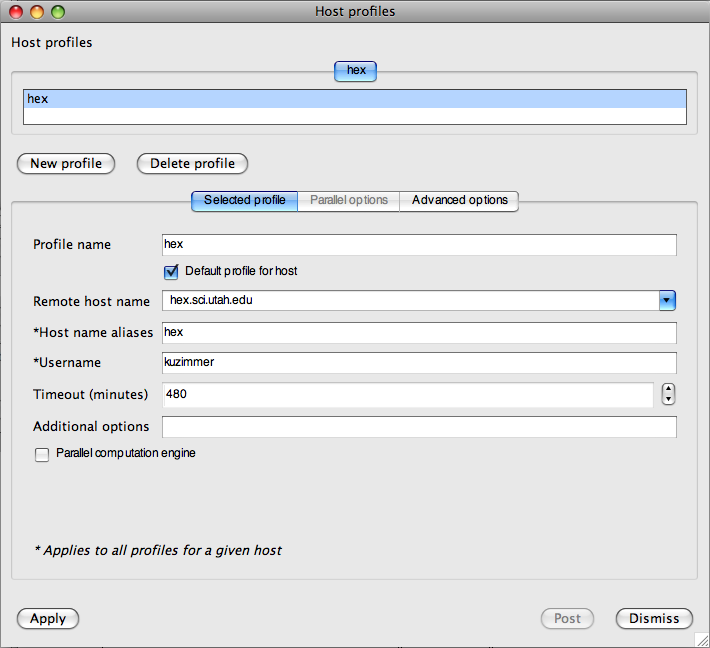
\includegraphics[width=.425\textwidth]{VisItHostProfile.png}
%   \end{center}
%   \vspace{-20pt}
%   \caption{Setting up Host Profile}
%   \vspace{-30pt}
%   \label{VisItHostProfile}
% %\end{figure}

% \end{wrapfigure}


\begin{wrapfigure}{r}{.50\textwidth}

%\begin{figure}
   \vspace{-25pt}
  \begin{center}
    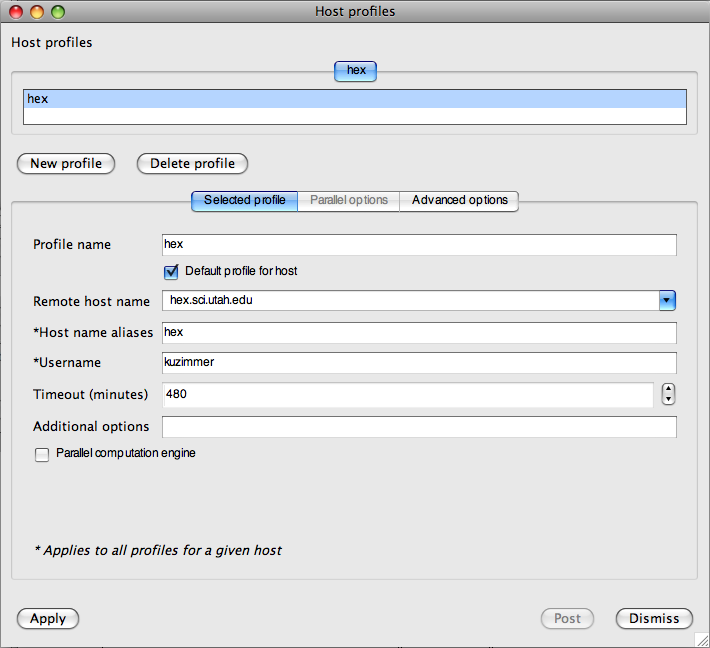
\includegraphics[width=.425\textwidth]{VisItHostProfile.png}
  \end{center}
  \caption{Setting up Host Profile}
   \vspace{-20pt}
  \label{VisItHostProfile}
%\end{figure}

\end{wrapfigure}


After filling in the remote machine information, select the 'Advanced
options' tab, then 'Networking' and check the 'Tunnel data connections
through SSH' option. This is illustrated in
figure~\ref{VisItHostProfileAdv}. Click on 'Apply' and then do a 'Save
Settings' in the 'Options' menu on the gui.

% \begin{wrapfigure}{r}{.50\textwidth}

% %\begin{figure}
%   \vspace{-30pt}
%   \begin{center}
%     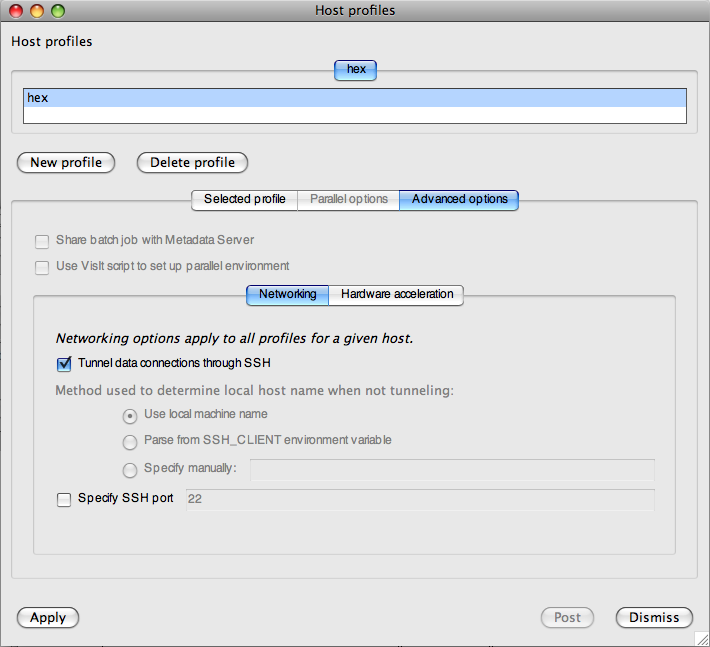
\includegraphics[width=.5\textwidth]{VisItHostProfileAdv.png}
%   \end{center}
%   \vspace{-20pt}
%   \caption{Setting up advanced options}
%   \vspace{-10pt}
%   \label{VisItHostProfileAdv}
% %\end{figure}

% \end{wrapfigure}

% \begin{wrapfigure}{r}{.50\textwidth}

% \begin{figure}

%   \begin{center}
%     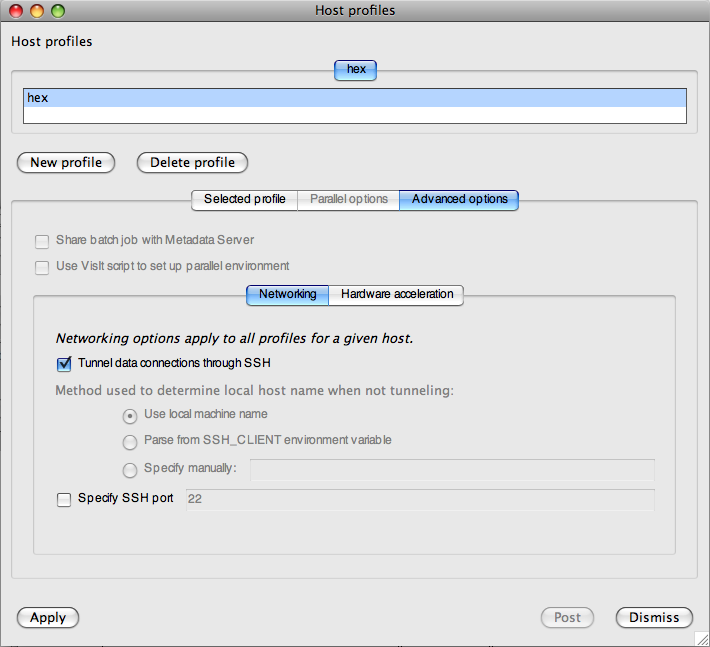
\includegraphics[width=.5\textwidth]{VisItHostProfileAdv.png}
%   \end{center}

%   \caption{Setting up advanced options}

%   \label{VisItHostProfileAdv}
% \end{figure}

% \end{wrapfigure}

\begin{wrapfigure}{r}{.50\textwidth}
%\begin{figure}[h]
  \centering
  \vspace{5pt}
  \subfloat[Setting up advance options]{\label{VisItHostProfileAdv}
    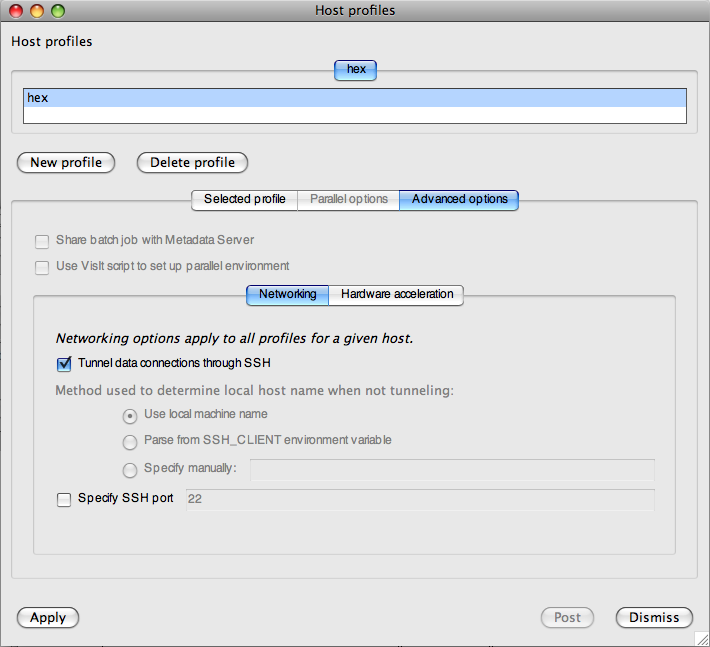
\includegraphics[width=.5\textwidth]{VisItHostProfileAdv.png}}
  \hspace{20pt}
  \subfloat[Setting up advance options]{\label{VisItHostProfileAdv2}
    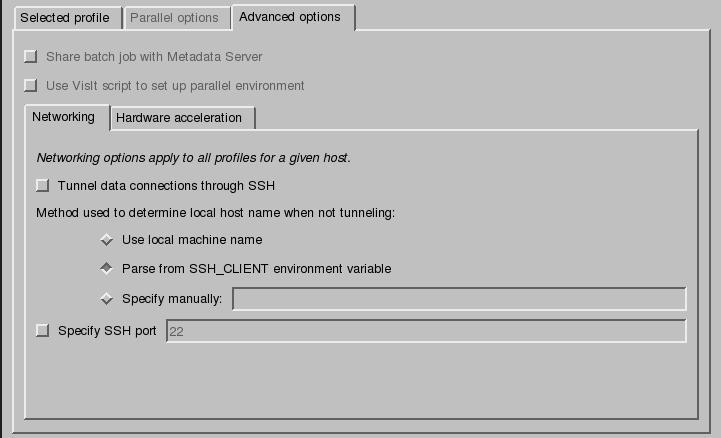
\includegraphics[width=.5\textwidth]{VisItHostProfileAdv2.png}}
  \caption{}
  \vspace{-10pt}
  \label{}
%\end{figure}
\end{wrapfigure}


For the remote visualization option to work, you must have ports 5600
- 5609 open. You can try this by running the following on your local
desktop (on Linux distributions),

\begin{lstlisting}
traceroute -p 560[0-9] <remote machine>
\end{lstlisting}

%\begin{wrapfigure}{r}{.50\textwidth}

% \begin{figure}
%   \vspace{-30pt}
%   \begin{center}
%     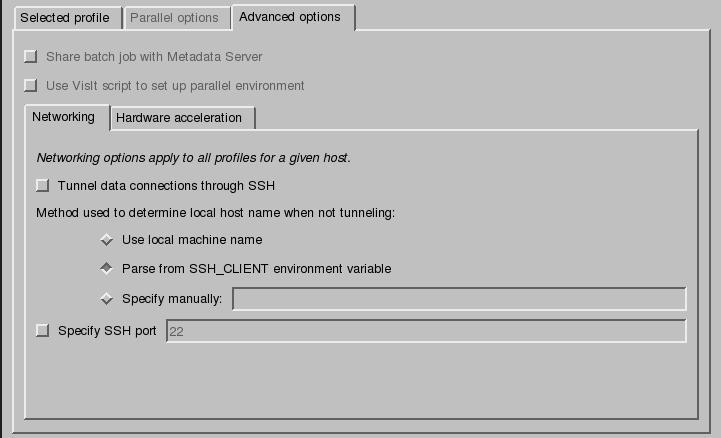
\includegraphics[width=.5\textwidth]{VisItHostProfileAdv2.png}
%   \end{center}
%   \vspace{-20pt}
%   \caption{Setting up advanced options}
%   \vspace{-10pt}
%   \label{VisItHostProfileAdv2}
% \end{figure}

%\end{wrapfigure}


If the tunneling option doesn't works, try the option as shown in
figure~\ref{VisItHostProfileAdv2}.



Now you should be able select 'Open' from VisIt's 'File' menu. After
selecting your host from the host entry list, you will be prompted for
a password on the remote machine (unless you have set up passwordless
ssh access).

Once the ssh login has completed, you should see the directory
listing. You can then change directories to your UDA and load the
data.


% \section{Manta Installation}

% For complete build instructions for Manta, please refer to
% \url{http://software.sci.utah.edu/manta/index.php/CSAFE}.  

% \begin{enumerate}
% \item
% Install Teem see~\ref{subsec:teem}.
% \item
% Install wxPython 2.8+ http://www.wxpython.org/ .  
% to verify that you have 2.8+ installed, run
% \begin{lstlisting}
% > python
% >>> import wxversion
% >>> wxversion.getInstalled()
% ['2.8-mac-unicode']
% \end{lstlisting}
% \item
% The next step is to download the Manta source and create a build directory.
% \begin{lstlisting}
% mkdir Manta
% mkdir Manta/build
% svn co https://code.sci.utah.edu/svn/Manta/trunk Manta/src
% \end{lstlisting}
% \item
% The build is configured with CMake.
% \begin{lstlisting}
% cd Manta/build
% ccmake ..
% \end{lstlisting}
% \item First you will need to set the TEEM library path. Press the down
%   arrow until you get to the variable FOUND\_TEEM\_BIN. Set this to
%   the location of your TEEM installation by pressing enter and
%   entering the path, eg /usr/bin. Press "c" to configure. If you get
%   errors about not finding TeemConfig.cmake (in older versions before
%   Nov. 2008 it was called TEEMConfig.cmake), you can manually set this
%   by pressing t and going down to the variable named
%   FOUND\_TEEMCONFIG\_CMAKE and setting it to TeemConfig.cmake from
%   your TEEM installation.
% \item You will need to enable the following by scrolling down to them
%   and pressing "enter" if they do not already say ON:
%   BUILD\_SWIG\_INTERFACE, BUILD\_NRRDPARTICLES, MANTA\_SSE. Now press
%   "c" to configure.
%  \item
%  You should now see an option called SCENE\_CSAFE, enable this if not already. Now press "c" to configure again. 
%  \item
%  Click "g" to generate the cmake files. you can now build Manta again by typing make. 
% \end{enumerate}


\chapter{Mac OSX Installation}

Following are step-by-step instructions for installing the
\textbf{Uintah Computational Framework} on \textbf{Mac OSX}.  It is
assumed that all commands are run as administrator (which may require
a sudo).  These instructions were tested on OSX 10.5.6 and 10.5.7 but
should work on previous versions.  \textbf{If you have Snow Leopard,
go to Section 10.}

\section{Installing Developer Tools}
Install the suite of developer tools that are packaged with Mac OS X.
These can be found in the "Optional Installs" directory on the Mac OS
X Installation CD for newer versions (i.e. Tiger, Leopard) or on the
included Developer CD if your version of OSX is older). If you don't
have the installation CD you can download older versions from:
\url{http://connect.apple.com}

Double-click the XCodeTools.mpkg and follow the installer
instructions.  This will install GCC, as well as many other useful
developer tools.

\section{Installing Fortran Compiler}
Download gfortran from \url{http://hpc.sourceforge.net/} making sure
the package is designed for your CPU architecture--Intel or PowerPC.
Put package in root directory and extract.  Extracting from / puts
everything in the correct places.  Extract using:

\begin{lstlisting}
	tar -xvf gfortran-*-bin.tar.gz
\end{lstlisting}

Note: If the Uintah builds correctly, but you are receiving link errors, see section 10.2.

\section{Installing Subversion/libpng3/libxml2/other dependencies}
As mentioned above, several libraries are required for Uintah, and may
need to be updated or installed depending on the version of Mac
running.  Some of these include SVN, libpng3, cmake, zlib and libxml2,
which are all conveniently part of the fink project.

Download the appropriate version of fink for your version of OSX from
\url{http://www.finkproject.org/download/srcdist.php}.  Where "x" and
"y" are version numbers, extract and install with:

\begin{lstlisting}
	tar -xvf fink-0.x.y-full.tar 
	cd fink-0.x.y-full
	./bootstrap 
	pathsetup.sh
\end{lstlisting}

For a GUI version of fink, download Fink Commander and install from
disk image from \url{http://finkcommander.sourceforge.net/} following
instructions in the installer.  The Fink Commander website stresses
that you install Commander after fink.

Finally, update or install any necessary packages using Fink
Commander's search bar.

\section{Install/Update X11}
X11 can be found in the "Optional Installs" directory accompanying
your Mac OS Installation CD.  This copy should be updated.
Alternately, X11 can be downloaded from the web and installed.
Current versions can be found at
\url{http://xquartz.macosforge.org/trac/wiki/Releases}.  Find a
package that matches your version of OSX (or update OSX to newest
version), and install it.  Installation is as simple as downloading
the disk image from this site, mounting it, double-clicking the
installer application, and following instructions.

\section{Installing an LAM MPI}
We recommend that you avoid using fink to install LAM MPI.
The files and libraries are installed in non-traditional locations 
and Uintah cannot find them. (11/10/2010) \\

Download LAM MPI from \url{http://www.lam-mpi.org}
version 7.1.4 or newer.  Make a new directory in \textasciitilde/ for
this and all of the following source packages.  This documentation
assumes this directory is \textasciitilde/Uintah.  Inside this
directory make another for installation directories.  This
documentation assumes this directory is
\textasciitilde/Uintah/installs

\begin{lstlisting}
	cd ~/Uintah/installs
	tar -xvf lam-7.1.4.tar.gz
	cd lam-7.1.4
	./configure --prefix=/Users/<username>/Uintah/installs/lam-7.1.4 \
	            --enable-shared=yes --with-fc=gfortran
	make
	make install
\end{lstlisting}

These last two commands will build LAM in the directory to which
--prefix= points.

\section{Installing PETSc}
PETSc and Hypre (the next two packages to install) are used by Uintah
for their PDE and linear algebra and capabilities respectively.
Download PETSc from
\url{http://www-unix.mcs.anl.gov/petsc/petsc-as/download/index.html}.
Unarchive it in \textasciitilde/Uintah/installs directory using a
similar tar command as is found above.  Configure using:

\begin{lstlisting}
	./config/configure.py \
	   --prefix=/Users/<username>/Uintah/installs/petsc-2.3.3-p13 \
	   --with-matlab=false \
	   --with-x=false \
	   --with-shared=0 \
	   --with-debugging=0 \
	   --with-mpi-dir=/Users/<username>/Uintah/installs/lam-7.1.4
\end{lstlisting}

Set the environmental variables the configuring process asks you to
set, and install using:

\begin{lstlisting}
make
make install
\end{lstlisting}

\section{Installing Hypre}
Download Hypre version 2.x from
\url{https://computation.llnl.gov/casc/hypre/software.html} to
\textasciitilde/Uintah/installs.  Unarchive and install by running

\begin{lstlisting}
cd hypre-2.x.x/src
./configure \
   --with-MPI-include=/Users/<username>/Uintah/installs/lam-7.1.4/include \
   --with-MPI-lib-dirs=/Users/<username>/Uintah/installs/lam-7.1.4/lib \
   --with-MPI-libs="mpi lam pmpi util" \
   --prefix=/Users/<username>/Uintah/installs/hypre-2.0.0/hypre_install \
   CFLAGS="-DMPIPP_H" \
   CXXFLAGS="-DMPIPP_H" 
make
make install
\end{lstlisting}

Take down of your --prefix line for future reference, as this is where
you will point Uintah's configure.

\section{Installing Uintah}
Download the Uintah source from our website using:

\begin{lstlisting}
cd ~/
svn co https://gforge.sci.utah.edu/svn/uintah/trunk ~/Uintah
\end{lstlisting}

Uintah will not install correctly if configured from within the source
directory.  As such, it is advised to create a directory on the same
level as /Uintah/src named mac[Numofbits]opt in which to configure and
build.

\begin{lstlisting}
cd Uintah
mkdir mac32opt
cd mac32opt
./configure \
   --enable-optimize \
   --with-mpi=/Users/<username>/Uintah/installs/lam-7.1.4 \
   --with-petsc=/Users/<username>/Uintah/installs/petsc-2.3.3-p13 \
   --with-hypre=/Users/<username>/Uintah/installs/hypre-2.0.0/hypre_install \
   PETSC_ARCH=darwin9.3.0-c-opt \
   F77=gfortran
\end{lstlisting}

The previous configure command is a template, and may need editing.
Point each of the components to the proper places and it should
configure just fine.  If you want to build Uintah with support for
VisIt, add --with-teem=/dir/to/teem/ and --with-visit=/dir/to/visit/
Finish the process off with:

\begin{lstlisting}
make all
\end{lstlisting}
  

Some useful programs can be found in the installation: sus will be
built and installed in \textasciitilde/Uintah/mac32opt/StandAlone
Extraction utilities that extract specific variables from UDA (Uintah
Data Archive) can be found in
\textasciitilde/Uintah/mac32opt/StandAlone/tools

\section{Installing VisIt and udaReader on Mac}

A Mac binary distribution is available from LLNL at
\url{https://wci.llnl.gov/codes/visit/executables.html}.  The main
difficulty in installing Uintah with udaReader plugin has to do with
actually finding the VisIt installation executable.  Furthermore,
naming conventions are slightly different, and thus several links must
be set up.

Extract the mac install and create links by (substitute i386 and VisIt
version where necessary):

\begin{lstlisting}
tar xvf visit1_11_2.darwin-i386.tar.gz
cd visit/1.11.2
export PATHTOVISIT=\$(pwd)
mkdir src
ln -s \$PATHTOVISIT/darwin-i386/bin src/bin
ln -s \$PATHTOVISIT/../bin/frontendlaucher src/bin/visit
\end{lstlisting}

Now that the links have been set up, configure Uintah with
--with-visit=\$PATHTOVISIT and --with-teem=DIR/TO/TEEM.  See Section
8.1 for Teem installation.

An easier solution is to download the VisIt directory from the Uintah
source, and run xml2makefile from \$PATHTOVISIT/darwin-i386/bin on
udareaderMTMD.xml within VisIt/udaReaderMTMD/udaREaderMTMD.xml such
as:

\begin{lstlisting}
xml2makefile -clobber -private VisIt/udaReaderMTMD/udaReaderMTMD.xml
\end{lstlisting}

To install VisIt from source, see build notes for Mac inside source
tarball.

\subsection{Installing VisIt and the udaReader on a Mac running OSX 10.6.1}

The following steps should allow one to build VisIt and the Uintah VisIt uda reader plug-in on a Macintosh running OsX 10.6.1 (Snow Leopard):
%
\begin{enumerate}
\item Obtain the VisIt source from:
\begin{lstlisting}
svn co http://portal.nersc.gov/svn/visit/trunk/src visit/src
\end{lstlisting}
\item \begin{lstlisting} cd visit/ \end{lstlisting}
\item \begin{lstlisting} mkdir third-party/ \end{lstlisting} (here we will compile all the third-party software needed by visit)
\item Manually download Python.2.6.4 
\begin{lstlisting}
http://www.python.org/
\end{lstlisting}
to third-party/
\item Manually download cmake 2.6.4 
\begin{lstlisting}
http://www.cmake.org/
\end{lstlisting}
to third-party/
\item Manually download qt-mac-opensource-src-4.5.3 
\begin{lstlisting}
http://get.qt.nokia.com/qt/source/qt-mac-opensource-src-4.5.3.tar.gz
\end{lstlisting}
to third-party/
\item Manually download VTK 5.0.0d 
\begin{lstlisting}
http://portal.nersc.gov/svn/visit/trunk/third_party/
\end{lstlisting}
to third-party/
\item Inside of third-party,
\begin{lstlisting}
cp ../src/svn-build/build_visit . 
\end{lstlisting}
\item Execute
\begin{lstlisting}
./build_visit --no-visit 
\end{lstlisting}
\item Edit the host.conf generated by build\_visit by adding: 
\begin{lstlisting}
-D__USE_ISOC99
\end{lstlisting} 
 to the CXXFLAGS variable. 
\item Copy the host.conf in the third-party/ directory to ../src/config-site/ 
\begin{lstlisting}
cp <some name>.conf ../src/config-site/
\end{lstlisting}
\item \begin{lstlisting} cd ../src/ \end{lstlisting}
\item \begin{lstlisting}./configure \end{lstlisting} 
\item \begin{lstlisting}make \end{lstlisting}
\item When the make fails with an error of not finding -lGLU, open databases/Shapefile/Makefile and replace -lGLU with -framework OpenGL
\item Type make again. It should finish successfully and the VisIt executable will be in visit/src/bin
\item Add 
\begin{lstlisting}
#define VERSION "2.1.0"
\end{lstlisting}  
to src/include/visit-config.h
\item Configure Uintah with (for example): 
\begin{lstlisting}
--with-visit=/Users/<path to visit>  \ 
--with-teem=/Users/<path to SCI thirdparty>/install
\end{lstlisting}
\item Build Uintah
\begin{lstlisting}
make -j# 
\end{lstlisting}
\end{enumerate}  
 % % % % % % % % % % % % % % % % % % % % % % % % % % % % % % % % % % % % % % % % % % % % % % % % % % % % % % % % % % % % % % % % % % % % % % % % % % % % % % % % % % % %
\chapter{Mac OSX Snow Leopard Installation (10.6.3)}
	What follows is a working configuration for installing Uintah on Mac OSX Snow Leopard (10.6.3) under 64 bit. In this example, it is assumed that Uintah is installed under
	\begin{lstlisting}
		/Users/username/uintah
	\end{lstlisting}
	Also, all packages will be downloaded and installed under 
	\begin{lstlisting}
		/Users/username/uintah/packages
	\end{lstlisting}

	\section{Fink}
		At the time of writing of this documentation, there is no binary version of the latest Fink distribution for Mac OSX. One must compile from the source by following the instructions on the website \url{http://www.finkproject.org/download/srcdist.php}. Make sure you select 64 bit mode when prompted. Keep all other options to default.
	
	\section{gfortran}
		Install the binary package for gfortran from: \url{http://r.research.att.com/tools/}. Then, set the path properly. If you are using bash, this is done as:
		\begin{lstlisting}
			export PATH=/usr/local/bin:$PATH
		\end{lstlisting}
		Note: If the Uintah builds correctly, but you receive a dynamic link error from fortran when you try to load a uda, the links in fortran library may be pointing to the wrong place.  This can easily be fixed by navigating to the fortran library and using "otool -L" to recognize the problem, then using install\_name\_tool to fix the problem.  Both are included in the mac developer tools.
	
	\section{openmpi}
		Download the latest version of openmpi from: \url{http://www.open-mpi.org/}. Then configure using:
		\begin{lstlisting}
			cd ~/uintah/packages
			tar -xvf openmpi-1.4.x
			cd openmpi-1.4.x
			./configure --prefix=/Users/username/uintah/packages/openmpi-1.4.x-install 
			\F77=gfortran CFLAGS=-m64 CXXFLAGS=-m64 FFLAGS=-m64
		\end{lstlisting}
		Then
		\begin{lstlisting}
			make
			make install
		\end{lstlisting}
		
		\section{hypre}
		Download the latest version of Hypre from here: \url{https://computation.llnl.gov/casc/hypre/software.html}. Then, configure using:
		\begin{lstlisting}
			cd ~/uintah/packages
			tar -xvf hypre-2.6.0b
			cd hypre-2.6.0b/src
			./configure --prefix=/Users/username/uintah/packages/hypre-2.6.0b-install 
												 \--with-MPI-include=/Users/username/uintah/packages/openmpi-1.4.x-install/include 
												 \--with-MPI-lib-dirs=/Users/username/uintah/packages/openmpi-1.4.x-install/lib 
												 \CC='gcc -arch x86_64' \CXX='g++ -arch x86_64' \F77='gfortran -arch x86_64' 
		\end{lstlisting}
		Then
		\begin{lstlisting}
			make
			make install
		\end{lstlisting}
		
		\section{PETSc}
		For the current release of Uintah, Petsc2.3.3 or Petsc2.2.0b has been found to work well. Download the source from here: \url{http://www.mcs.anl.gov/petsc/petsc-as/download/index.html}.
		Then browse to the packages directory and configure as follows:
		{\small
		\begin{lstlisting}
			cd ~/uintah/packages
			tar -xvf petsc-2.x.y-p15.tar.gz
			cd petsc-2.x.y-p15
			./config/configure.py \--with-shared \--with-debugging=0 
			\--with-mpi-include=/Users/username/uintah/packages/openmpi-1.4.x-install/include 
			\--with-mpi-lib=/Users/username/uintah/packages/openmpi-1.4.x-install/lib/libmpi.dylib 
			\--without-fortran \--prefix=/Users/username/uintah/packages/petsc-2.x.y-p15-install
		\end{lstlisting}}
		Finally,
		{\small
		\begin{lstlisting}
			PETSC_DIR=/Users/username/uintah/packages/petsc-2.x.y-p15-install; export PETSC_DIR
			make all test
			make install
		\end{lstlisting}}
		
		\section{Uintah}
		Finally, create a directory in uintah
		{\small 
		\begin{lstlisting}
			mkdir ~/uintah/mac64opt
		\end{lstlisting}} %
		\noindent Now browse to the mac64opt directory and configure Uintah using the following:
		\emph{Note, under Mac OSX 10.6, the build has to be 64-bit.}
		{\small
		\begin{lstlisting}
			cd ~/uintah/mac64opt
			../src/configure --with-mpi=/Users/username/uintah/packages/openmpi-1.4.1-install 
			\--with-hypre=/Users/username/uintah/packages/hypre-2.6.0b-install 
			\--with-petsc=/Users/username/uintah/packages/petsc-2.3.3-p15-install 
			\--enable-optimize='-O2' \--enable-64bit 
			CC=gcc CXX=g++ F77=gfortran CFLAGS=-m64 CXXFLAGS=-m64 FFLAGS=-m64
			PETSC_ARCH=darwin10.3.1-c-opt USE_ICE=yes USE_MPM=yes
		\end{lstlisting}} %
		\noindent Finally
		{\small
		\begin{lstlisting}
			make all
		\end{lstlisting}}
\chapter{Appendix: Teem Installation}

\label{subsec:teem}

\emph{ \textbf{Note:}Teem is only needed for UdaToNrrd (which is used to
  translate UDA into NRRD files for visualization with the Manta or
  RTRT ray tracers.  Users of \textbf{\emph{VisIt}} do not need to install Teem.}

Download Teem from
\url{http://teem.sourceforge.net/download/index.html}.  Teem uses
CMake to configure the build system. Installation instructions for
Teem are found at \url{http://teem.sourceforge.net/build.html}.
Simplified instructions are as follows:

\begin{lstlisting}
tar zxf teem-1.10.0-src.tar.gz
cd teem-1.10.0-src/
mkdir teem-build
cd teem-build
ccmake ../
\end{lstlisting}

Use the arrow keys to scroll down to the fourth line
BUILD\_SHARED\_LIBS and press the return key to toggle the ON flag.

\begin{lstlisting}
Press the 'c' key

Press the 'g' key

make
make install
\end{lstlisting}
The Teem libraries and include files will be install in /usr/local
hierarchy.  If you have a /usr/local/lib64 directory please make a
symbolic link to the libteem.so found in /usr/local/lib, i.e.

\begin{lstlisting}
cd /usr/local/lib64
ln -s ../lib/libteem.so libteem.so
\end{lstlisting}

After Teem has been installed then add the location of your Teem
install to the \textbf{Uintah} as in:

\begin{lstlisting}
--with-teem=/usr/local
\end{lstlisting}

  
%----------------------------------------------------------------------------------------
%       BIBLIOGRAPHY
%----------------------------------------------------------------------------------------

\chapter*{Bibliography}
\addcontentsline{toc}{chapter}{\textcolor{ocre}{Bibliography}}

%\bibliographystyle{plain}
%\bibliography{Bibliography}
\printbibliography[heading=bibempty]



\end{document}
